\chapter{Theorie}\label{theorie}

\section{Diskurslinguistik}\label{diskurslinguistik}

\subsection{Verortung in der Linguistik}\label{verortung-in-der-linguistik}

Kulturbezogene Untersuchungsgegenstände wie Diskurse und die in ihnen verhandelten Themen sowie das Wissen, das Diskursteilnehmende benötigen, um sich in ihnen zu orientieren und einzubringen, können heute als etablierter Teil der Linguistik gelten. Warum es gerechtfertigt ist, den Diskurs als „sprachwissenschaftliches Objekt`` \autocite{busseIstDiskursSprachwissenschaftliches1994} aufzufassen, was überhaupt unter Diskursen zu verstehen ist und was sprachwissenschaftliche Analysen „im interdisziplinären Verbund der Diskursanalyse`` \autocite[10]{spitzmullerDiskurslinguistikEinfuhrungTheorien2011} beitragen können, soll in diesem Kapitel geklärt werden.

In ihrem einschlägigen Aufsatz „Ist Diskurs ein sprachwissenschaftliches Objekt?{}`` \autocite{busseIstDiskursSprachwissenschaftliches1994} plädieren die Linguisten Dietrich Busse und Wolfgang Teubert für eine Beschäftigung mit Diskursen (im Sinne der französischen Diskursanalyse nach Foucault) in der germanistischen Sprachwissenschaft. Fasst man als Konstituenten von Diskursen, wie es laut Gardt \autocite*[30]{gardtDiskursanalyseAktuellerTheoretischer2007} in den Philologien üblich ist, „Äußerungen und Text{[}e{]} der unterschiedlichsten Art`` zu einem Thema auf, so könnte man auf die von Busse und Teubert aufgeworfene Frage zunächst entgegnen: „Warum denn nicht?{}`` – könnte man doch annehmen, dass die Analyse eines möglicherweise nicht ausschließlich, aber doch ganz wesentlich sprachlich in Texten konstituierten Gegenstandes natürlicher Bestandteil der sprachwissenschaftlichen Forschung sei. Nichtsdestoweniger muss das Analyseinteresse an einem neuen Gegenstand -- und das waren Diskurse im Foucaultschen Sinne zum Zeitpunkt der Veröffentlichung von Busse \& Teubert \autocite*{busseIstDiskursSprachwissenschaftliches1994} für die germanistische Linguistik -- gerechtfertigt werden -- und dies, wie von Spitzmüller und Warnke \autocite*{spitzmullerDiskurslinguistikEinfuhrungTheorien2011} in aller Ausführlichkeit praktiziert, in zwei Richtungen: Zum einen muss die Diskurslinguistik erklären, warum der Diskurs ein Analyseobjekt für die Sprachwissenschaft ist und wie er sich zu den Gegenständen der bereits bestehenden Teildisziplinen wie der Syntax oder Textlinguistik verhält. Zum anderen muss herausgestellt werden, was die Linguistik im Vergleich zu anderen Disziplinen, die schon länger diskursanalytisch arbeiten, wie z.\,B. die Kulturwissenschaft, an neuen Erkenntnissen beitragen kann. Zur Beantwortung dieser Fragen soll in diesem Kapitel zunächst der in dieser Arbeit verwendete Diskursbegriff geklärt werden, bevor ich das Konzept semantischer Frames darstelle, die eine elementare Rolle für das Handeln in Diskursen einnehmen.

\subsection{Diskursbegriff und methodologische Zugänge zum Diskurs}\label{diskursbegriff-und-methodologische-zugaenge-zum-diskurs}

Spitzmüller und Warnke \autocite*[9]{spitzmullerDiskurslinguistikEinfuhrungTheorien2011} unterscheiden vier wesentliche Diskursbegriffe, die in der Linguistik gebraucht werden: einen bildungssprachlichen Diskursbegriff, der in den Medien synonym für ‚Debatte` oder ‚Gespräch` verwendet werde; den Habermasschen Diskursbegriff, der von ihm als Teil eines „kommunikationsethischen Programms`` entworfen wurde; den Diskursbegriff der anglo-amerikanischen \emph{discourse analysis}, der auch in der germanistischen Diskursanalyse zur Beschreibung größerer Einheiten der interaktiven gesprochenen Sprache verwendet wird und letztlich einen an Foucault orientierten poststrukturalistischen Diskursbegriff, wie er auch im Rahmen der vorliegenden Arbeiten verwendet wird. Letzteren beschreiben sie als „Formationssystem von Aussagen, das auf kollektives, handlungsleitendes und sozial stratifizierendes Wissen verweist`` \autocite[9]{spitzmullerDiskurslinguistikEinfuhrungTheorien2011}. Es ist dieser Diskursbegriff, der für die mittlerweile etablierte Diskurslinguistik prägend ist, die im Titel von Warnke \autocite*{warnkeDiskurslinguistikNachFoucault2007} auch als „Diskurslinguistik nach Foucault`` bezeichnet wird. Gardt präsentiert in diesem Band eine Diskursdefinition, die er induktiv aus den in den Philologien zugrundegelegten Diskursdefinitionen, die zumindest „mehr oder weniger deutlich in der Tradition Michel Foucaults stehen`` \autocite*[28]{gardtDiskursanalyseAktuellerTheoretischer2007}, kondensiert:

\begin{quote}
Ein Diskurs ist die Auseinandersetzung mit einem Thema,\\
- die sich in Äußerungen und Texten der unterschiedlichsten Art niederschlägt,\\
- von mehr oder weniger großen gesellschaftlichen Gruppen getragen wird,\\
- das Wissen und die Einstellungen dieser Gruppen zu dem betreffenden Thema sowohl spiegelt\\
- als auch aktiv prägt und dadurch handlungsleitend für die zukünftige Gestaltung der gesellschaftlichen Wirklichkeit in Bezug auf dieses Thema wirkt. \autocite[30]{gardtDiskursanalyseAktuellerTheoretischer2007}
\end{quote}

Mit der Ausrichtung an Foucault gehen also gewisse poststrukturalistische Annahmen über die Entstehung einer gemeinsamen gesellschaftlichen Wirklichkeit einher. Insbesondere soziale Konzepte wie ‚Extremismus` sind in diesem Verständnis nicht einfach ‚irgendwie da` oder mit einem objektiven inhaltlichen Kern versehen. Sie sind vielmehr das Ergebnis eines auf Diskursebene zwischen den Individuen verhandelten Wissens. Wie in der Definition festgehalten, wirkt dieses Wissen in zwei Richtungen: Zum einen greifen Menschen darauf zurück, um sich in der Welt zu orientieren und miteinander zu kommunizieren, sodass es sich auf Diskursebene „spiegelt`` und aufspüren lässt. Zum anderen formen Menschen es in der Interaktion im Diskurs immer wieder neu und werden werden durch dieses Wissen geleitet, da Diskurse immer auch machtvoll strukturiert sind und „handlungsleitend`` auf die Individuen wirken.

Ein deutlich anders ausgerichteter Diskursbegriff wurde in der datengeleiteten, quantitativen Diskurslinguistik vorgeschlagen. So definiert Bubenhofer Diskurse nicht themenbasiert, sondern entlang von rekurrentem, musterhaftem Sprachgebrauch, sogenannten Sprachgebrauchsmustern:

\begin{quote}
Zweitens versuchte ich das rekurrente Auftreten (die musterhafte Verwendung dieser Wortverbindungen) als ‚Sprachgebrauchsmuster` zu lesen, die Indikatoren für die Gestalt von Diskursen darstellen. Denn im Anschluss an Foucault (1981) formen die Prozeduren der Produktion des Diskurses das inhaltlich Sagbare, sowie die Sprechweisen, also die diskursive Praxis. Diese diskursive Praxis ist nichts anderes als die regelmäßige, eben: musterhafte Art des Aussagens. \autocite[309]{bubenhoferSprachgebrauchsmusterKorpuslinguistikAls2009}
\end{quote}

Es wird deutlich, dass sich Bubenhofer dabei ebenfalls an Foucault orientiert, jedoch den Sprachgebrauchsmustern auf der Textoberfläche, die er mit Linke \autocite*[40]{linkeBegriffsgeschichteDiskursgeschichteSprachgebrauchsgeschichte2003} als „minimale Kristallisationskerne`` von Diskursen bezeichnet, den Stellenwert des Bindegliedes zwischen den „Äußerungen und Texten der unterschiedlichsten Art``, wie es bei Gardt \autocite*[28]{gardtDiskursanalyseAktuellerTheoretischer2007} heißt, einräumt. Damit wird ein thematischer Zusammenhang der zum Diskurs gehörigen Texte, der in der philologischen Diskursforschung primäres Definitionskriterium war, zwar nicht ausgeschlossen, jedoch zu einem sekundären Kriterium. Die Motivation dieser Definition liege im induktiveren und weniger voreingenommenen Zugang zum Diskurs, der so ermöglicht werde:

\begin{quote}
Die Frage nach der Repräsentativität des Korpus zeigt, dass Busse{\slash}Teubert (1994, 14f.) diese nach inhaltlichen Kriterien festlegen, was zu einer manuellen Auswahl von „relevanten`` Texten führt. Diese Beschränkung ist nicht nur unnötig, sondern auch kritisch, wenn das Ziel einer Diskursanalyse darin besteht, auch verborgene und unauffällige Strukturen aufzuzeigen. Relevanzempfinden ist ein Ergebnis diskursiver Formationen. Dieses als Kriterium zu wählen, bedeutet, die offensichtlichen Strukturen des Diskurses zu replizieren. \autocite[36]{bubenhoferSprachgebrauchsmusterKorpuslinguistikAls2009}
\end{quote}

Neben dem divergenten Diskursbegriff zeigen sich hier auch die damit einhergehenden methodologischen Differenzen. So finden sich in der germanistischen Diskurslinguistik einerseits Positionen, wie die hier von Bubenhofer vorgetragene oder die von Scharloth et al. \autocite*{scharlothWuchernRhizomeLinguistische2013}, die das Korpus ins Zentrum des Forschungsvorhabens stellen. Dabei wird in provokanter Weise nicht nur die thematische Diskursdefinition durch eine induktive, auf Sprachgebrauchsmustern basierende ersetzt; es wird auch der Einsatz sehr großer Korpora gefordert, um gemäß quantitativer Gütekriterien validere und realiablere Ergebnisse zu erhalten. Zugleich wird auch die in der Diskurslinguistik vorherrschende und auf qualitativer Lektüre einzelner Texte basierende Kategorienbildung abgelehnt. Vor dem Hintergrund dieser gänzlich anderen Forschungszugänge und -möglichkeiten geht es den Vertretern dieses Paradigmas dann auch darum, den korpuslinguistischen Zugang nicht als bloße Methodenfrage zu begreifen, sondern als „eigene Perspektive`` auf Sprache \autocite[2 unter Bezug auf Tognini-Bonelli 2001: 84]{perkuhnKorpuslinguistikUnbekannteWesen2006} bzw. als „eigenständigen Denkstil, der die Aspekte der Empirie, Quantität und Textorientierung miteinander verbindet`` \autocite[148]{bubenhoferKorpuslinguistischeDiskursanalyseNutzen2013}.

Ob sich die thematische Definition eines Diskurskorpus und eine induktive, sprachoberflächliche Phänomene fokussierende Herangehensweise ausschließen, ist eine der noch zu diskutierenden Fragen dieser Arbeit. Bevor sie beantwortet werden kann, soll jedoch beleuchtet werden, wie das „Wissen und die Einstellungen`` der „mehr oder weniger großen gesellschaftlichen Gruppen`` \autocite[28]{gardtDiskursanalyseAktuellerTheoretischer2007} zunächst theoretisch beschrieben werden können. Dafür wird Dietrich Busses \autocite*{busseFrameSemantikKompendium2012} Konzept semantischer Frames herangezogen, das im folgenden Kapitel in Hinblick auf die Rolle, die es in der linguistischen Diskursanalyse einnehmen kann, beleuchtet wird, bevor es in \chapref{das-frame-konzept-dietrich-busses} ausführlicher dargestellt wird.

\subsection{Frames als Elemente diskursiven Wissens}\label{frames-als-elemente-diskursiven-wissens}

Wie zuvor gesagt, stellt die Beschreibung und Modellierung von in Diskursen ausgehandeltem Wissen einen zentralen Bestandteil der linguistischen Diskursanalyse dar. Insbesondere Dietrich Busse plädiert dafür, sich in der Linguistik diesen Fragen zu widmen und benennt als Ziel einer solchen ‚linguistischen Epistemologie` die „linguistisch reflektiert{[}e{]} Erforschung der Rolle des bedeutungs- und verstehensrelevanten Wissens in seinem/r ganzen Umfang und Struktur`` \autocite*[190-191]{busseSprachverstehenUndTextinterpretation2015}. Bei der Art und Weise, wie einzelne Wissenselemente dabei modelliert werden, sind sowohl innerhalb der Linguistik als auch im Vergleich zu den Kultur- und Sozialwissenschaften Unterschiede festzustellen, jedoch auch weitgehende Übereinstimmungen. So konstatiert etwa Zabel \autocite*[66]{zabelSpracheKulturWiderstand2015}, dass man in den „Sozial- und Sprachwissenschaften {[}\ldots{]} je nach disziplinärer Interessenlage ein breites Sammelsurium an Begrifflichkeiten verwendet {[}hat{]}, die alle mehr oder weniger explizit als orientierende kulturelle Wissensmuster aufgefasst werden können``; darunter zählt sie die Konzepte ‚Stereotyp`, ‚Topos und Argumentationsmuster`, ‚Rahmen und Frame`, ‚Sinn- und Orientierungsmuster` sowie ‚(kulturelle) Deutungsmuster`. Auch der bereits mehrfach erwähnte Begriff des ‚semantischen Frames` stellt also ein solches Wissensmuster dar und wird von seinem Schöpfer Charles J. Fillmore in ähnlicher Stoßrichtung als eines der „many organized packages of knowledge, beliefs, and patterns of practice that shape and allow humans to make sense of their experiences`` \autocite[314]{fillmoreFramesApproachSemantic2010} gefasst. Fillmore entwickelt sein Frame-Konzept zeitlich parallel zum Kognitionswissenschaftler Marvin Minsky, wobei beide an die Schematheorie des Psychologen Frederick C. Bartlett anknüpfen. Entwicklungsschritte, Gemeinsamkeiten und Divergenzen der einzelnen Frame-Ansätze werden ausführlich von Busse \autocite*{busseFrameSemantikKompendium2012} herausgearbeitet. Dabei beleuchtet er neben Fillmore und Minsky etwa auch die Frame-Theorien Schank und Abelsons, Barsalous sowie der Schule Konerdings.\footnote{Es werden dabei nur Frame-Modelle mit einer Slot-Filler-Struktur beachtet. Das sozialwissenschaftliche Frame-Modell von Goffman \autocite*{goffmanFrameAnalysisEssay1974} etwa wird ausgespart.} Er entwickelt außerdem für die linguistische Epistemologie ein eigenes Frame-Modell, das auf den bestehenden Modellen basiert, sie integriert und weiterentwickelt.

Im Gegensatz zu anderen Modellen kultureller Wissensmuster bzw. den in den Kultur- und Sozialwissenschaften unternommenen Diskursanalysen rückt für die linguistische Diskursanalyse insbesondere der Bezug sprachlicher Zeichen zu diesen Wissenselementen in den Fokus. Ziel einer linguistischen Epistemologie ist es dabei immer, das gesamte verstehensrelevante Wissen, das zum Verständnis von sprachlichen Äußerungen notwendig ist, zu rekonstruieren und in Bezug zu den verwendeten sprachlichen Zeichen zu setzen. Dies grenzt die Frame-Semantik im Sinne Busses deutlich von traditionellen Semantiktheorien, aber zum Teil auch von einem Frame-semantisch-lexikographischen Zugang, wie er im \emph{FrameNet}-Projekt verfolgt wird (siehe \chapref{framenet} und \ref{warum-frames}), ab. Er konstatiert:

\begin{quote}
Der Bereich des in einer semantischen Analyse, die adäquat sein will, zu erfassenden bedeutungsrelevanten Wissens muss sehr viel weiter gezogen werden, als dies in der Linguistik und Sprachphilosophie bisher der Fall ist. Oder anders gesprochen: Gegenstand einer linguistischen Semantik muss immer die Gesamtheit des für das angemessene Verstehen eines sprachlichen Mittels bei den Verstehenden notwendigerweise vorauszusetzenden (von ihnen zu aktivierenden) Wissens sein. Dieses Wissen nenne ich das \emph{verstehensrelevante Wissen} (oder das bedeutungsrelevante Wissen). Semantik ist damit gleichzusetzen mit einer Analyse des gesamten verstehensrelevanten Wissens, das von einem sprachlichen Zeichen oder einer bestimmten Zeichenkombination (bis hin zu Sätzen und Texten) evoziert wird. Semantik wird damit zum Teil einer (umfassenderen) Wissensanalyse, die ich -- in Wiederaufnahme der ursprünglichen wörtlichen Bedeutung dieses Terminus -- \emph{Epistemologie} nenne. Soweit diese Wissensanalyse von Linguisten und mit linguistischen Mitteln betrieben wird, kann man eine solche Forschung dann als \emph{linguistische Epistemologie} bezeichnen. In diesem Sinne wird die Frame-Semantik zu einem wichtigen, wenn nicht zentralen, Baustein einer so verstandenen linguistischen Epistemologie. \autocite[805-806]{busseFrameSemantikKompendium2012}
\end{quote}

Es lässt sich zusammenfassen, dass in Diskursen Wissensbestände konstruiert, verhandelt und von Individuen in der Interaktion sowie zur Orientierung in der Welt genutzt werden. Ein wesentliches Ziel linguistischer Diskursanalysen -- und gerade für Busse auch der Semantik bzw. der linguistischen Epistemologie generell -- muss es sein, dieses Wissen nicht nur ‚als solches`, sondern auch präzise in seinem Zusammenhang mit Sprache zu modellieren. Als Modell für an sprachliche Zeichen rückgebundene Wissenselemente, das die Komplexität und Breite des Wissens (auch im Sinne einer Visualisierbarkeit) sichtbar macht, eignet sich sein Modell semantischer Frames.

Bevor das Frame-Konzept Busses näher beleuchtet wird, soll zunächst Fillmores Frame-Entwurf als erste linguistische Frame-Theorie dargestellt werden. Ich möchte so zum einen die historische Entwicklung der Frame-Semantik zumindest in Grundzügen nachzeichnen -- einen hervorragenden und umfassenden Überblick gibt Busse \autocite*{busseFrameSemantikKompendium2012} -- und zum anderen aufzeigen, inwiefern es notwendig ist, von diesem in der Linguistik sehr bekannten und vergleichsweise etablierten Frame-Konzept zugunsten eines deutlich komplexeren und schwerer handhabbaren Modells abzuweichen (siehe zur Begründung dann ausführlicher \chapref{warum-frames}).

\section{Frame-Semantik}\label{frame-semantik}

\subsection{Fillmores Frame-Semantik}\label{fillmores-frame-semantik}

\subsubsection{Entailment, Case Grammar, Understanding Semantics}\label{entailment-case-grammar-understanding-semantics}

Busse \autocite*[211-213]{busseFrameSemantikKompendium2012} gliedert Fillmores Werk in fünf Phasen: (1) die \emph{entailment}-Phase, in der Fillmore grundlegende Gedanken dazu formuliert, dass einzelne Sätze eigentlich weit mehr aussagen bzw. mehr Wissen voraussetzen, als es die zeitgenössischen Semantik-Theorien erklären können; (2) die Entwicklung der Tiefenkasus-Theorie, die an die europäische Valenz-Theorie Tesnières \autocite*{tesniereElementsSyntaxeStructurale1959} anknüpft, und erstmals den Begriff des \emph{Frames} verwendet, wenn auch zu dem Zeitpunkt noch im Sinne der Kasus-Rahmen als „abstrakte Entitäten auf der Ebene des generellen grammatischen und lexikalischen Wissens`` \autocite[212]{busseFrameSemantikKompendium2012} und nicht als epistemische Einheiten; (3) die kurze \emph{scenes-and-frames}-Phase, in der Fillmore den Begriff der Szene als ein eher auf die außersprachliche Welt und \emph{common-sense}-Wissen bezogenes Konzept einführt, das mit den eher sprachlich konzeptualisierten Frames zusammenwirkt; (4) die Phase der \emph{interpretive} oder \emph{understanding semantics}, in der der Frame-Begriff in einem umfassenderen und weniger lexikographisch interessierten Sinne verwendet wird. Es geht in dieser Phase um die „‚vollständige` Erfassung des ‚vollen Sets` von Bedingungen des adäquaten Verstehens``, anstatt nur explizit sprachlich Ausgedrücktes in die Analyse einzubeziehen \autocite[212]{busseFrameSemantikKompendium2012}, und letztlich (5) die \emph{FrameNet}-Phase, in der einerseits der Frame-Begriff etwa durch die Beschreibung von Strukturelementen wie den Frame-Elementen (FE) und lexikalischen Einheiten (LE) sowie Vererbungsrelationen weiterentwickelt wird und andererseits insbesondere die korpusbasierte und darstellungsorientierte Beschreibung von Frames in Form einer Datenbank fokussiert wird. Im Folgenden sollen diese fünf Schaffensphasen in einem kurzen Überblick vorgestellt werden, wobei ich mich an den Darstellungen in Busse \autocite*{busseFrameSemantikKompendium2012} orientiere.

\emph{Entailment}: Die Benennung dieser Phase von Fillmores Werk geht auf den Titel seines Aufsatzes „Entailment Rules in a Semantic Theory`` \autocite*{fillmoreEntailmentRulesSemantic1965} zurück. In diesem arbeitet Fillmore an verschiedenen Beispielen heraus, dass die Semantik von Sätzen durch die vorherrschende linguistische Bedeutungstheorie seiner Zeit von Katz \& Fodor \autocite*{katzStructureSemanticTheory1963}, die an die generative Grammatik Chomskys anknüpft, nicht vollständig erklärt werden können. Fillmore fasst diese Theorie wie folgt zusammen:

\begin{quote}
Each lexical item in the deep structure has associated with it, furthermore, both an assembly of semantic features corresponding to each possible reading (each sense) of the item, and a statement of the conditions under which each of these readings is selected. A semantic theory, in this view, provides a system of rules for projecting from the deep-structure representation of sentences to one or more semantic interpretations, matching, if it is correct, the judgments of the speakers of the language. \autocite[61-62]{fillmoreEntailmentRulesSemantic1965}
\end{quote}

Mit ihrer Hilfe könnten jedoch zwei semantische Phänomene nicht ohne Weiteres beantwortet werden. Einerseits sind dies „the so-called `relational` concepts`` \autocite[64]{fillmoreEntailmentRulesSemantic1965}, die von Fillmore durch Komparativsätze veranschaulicht werden. So müsse ein Satz wie „I am two years older than my father`` als „semantically odd`` (Fillmore 1965: 64) gelten, da die durch „my father`` und „older than`` ausgedrückten zeitlichen Verhältnisse konfligieren würden. Eine „bizarreness``, wenn auch semantische Intaktheit, konstatiert er dem Satz „My father is two years older than I am``:

\begin{quote}
The bizarreness of the sentence `I am two years older than my father' is quite different from whatever it is that's odd about `My father is two years older than I am.' If you hear the latter sentence, you may not believe it, or you may suspect that it was spoken by, say, a cat. But semantically, there is nothing wrong with it. \autocite[64]{fillmoreEntailmentRulesSemantic1965}
\end{quote}

Ein weiteres Beispiel ist für ihn der Satz „John is tall``, in dem kein Vergleichsobjekt expliziert ist. Hier müsse die Semantiktheorie den Satz um einen impliziten Vergleichswert ergänzen, der hier zu verstehen sei als „than average``, wobei das „universe of discourse`` \autocite[65]{fillmoreEntailmentRulesSemantic1965}, also die Werte, aus denen sich dieser Durchschnitt berechnen würde, im Satz nicht näher spezifiziert werden. Das zweite semantische Phänomen, das weder von Katz und Fodor noch durch die relationalen Konzepte erfasst werde, benennt Fillmore dann als \emph{entailment}. Durch \emph{entailment rules} werden die Sätze, die von den „ordinary semantic rules`` \autocite[65]{fillmoreEntailmentRulesSemantic1965} nicht erfasst werden, in eine Reihe von Sätzen übersetzt, die dann wiederum durch die etablierten semantischen Regeln erfasst werden können. Dies macht er u.\,a. an der Fokuspartikel \emph{even} deutlich, die im Satz „John is even taller than Bill`` \autocite[68]{fillmoreEntailmentRulesSemantic1965} eine Übersetzung in zwei Sätze im Sinne des \emph{entailment} notwendig mache, um zu erklären, warum der Satz semantisch enthält, dass auch Bill groß ist:

\begin{quote}
In the second sentence, the presence of `even' entails that Bill is tall. I would say that `John is even taller than Bill' entails the two sentences, `John is taller than Bill' and `Bill is tall.' Recall that `Bill is tall,' now, is to be interpreted as `Bill is taller than average.' \autocite[68]{fillmoreEntailmentRulesSemantic1965}.
\end{quote}

Mit dem Begriff des \emph{entailment} versucht Fillmore also auf wesentliche Defizite der Semantiktheorien seiner Zeit aufmerksam zu machen, insbesondere darauf, dass sich die Semantik eines Satzes nicht immer nur aus seiner grammatischen Tiefenstruktur und den semantischen Merkmalen der einzelnen Wörter rekonstruieren lässt -- auch wenn er daran als grundsätzlicher Herangehensweise festhalten möchte, die nur im Bedarfsfall durch \emph{entailment rules} komplettiert werden müsse \autocite[82]{fillmoreEntailmentRulesSemantic1965}. Auch wenn er es an dieser Stelle noch nicht so benennt, zeigen seine Ausführungen, dass auch kulturelles und nicht im engeren Sinne sprachliches Wissen zur Bedeutung eines Satzes beitragen kann, wie im Beispiel der durchschnittlichen Größe von Menschen oder der Gebärfähigkeit von Menschen und Katzen deutlich wird.\footnote{Wobei er Zweiteres ja -- ohne dies näher zu begründen -- (noch) nicht in den näheren Zuständigkeitsbereich der Semantik einschließen möchte und dem Satz „My father is two years older than I am.`` nur eine „bizarreness`` \autocite[64]{fillmoreEntailmentRulesSemantic1965} konstatiert.}

\emph{Deep cases} und \emph{case grammar}: In dieser Phase entwickelt Fillmore das Modell der Tiefenkasus und die Kasusgrammatik, die ihn international in der Linguistik berühmt gemacht hat und die als eine „‚Semantisierung der Syntax' (bzw. der Grammatik)`` \autocite[34]{busseFrameSemantikKompendium2012} begriffen werden kann. Fillmore stellt in dieser Phase den etablierten syntaktischen Kasus sogenannte Tiefenkasus bzw. Kasus-Rollen zur Seite, die heute i.d.R. als ‚semantische Rollen` bezeichnet werden, wie z.\,B. Agentiv, Instrumental, Dativ, Faktitiv usw. \autocite[24-25]{fillmoreCaseCase1968}. So weist „John`` in den synonymen Sätzen „John opened the door.`` und „The door was opened by John.`` zwar an der Oberfläche unterschiedliche Kasus auf und Subjekt und Objekt werden getauscht; der Tiefenkasus (\emph{deep case}) Agentiv bleibt jedoch identisch \autocite[25]{fillmoreCaseCase1968}. Die vom Verb bzw. zunächst dem Satz vorgegebene Struktur bezeichnet er dann als Kasus-Rahmen (\emph{case frame)}:

\begin{quote}
I have stated that A {[}Agentive, T.F.{]} and D {[}Dative, T.F.{]} are `animate' participants in the activity of the associated verbs, and I have also suggested that verbs are selected according to the case environments the sentence provides--what I shall refer to as the `case frame'. \autocite[26]{fillmoreCaseCase1968}
\end{quote}

Es setzt sich hier also der bereits in der \emph{entailment}-Phase beginnende rote Faden fort, die Relevanz semantischer Aspekte für die Beschreibung des Sprachsystems hervorzuheben.

Es folgt die \emph{scenes-and-frames}-Phase, in der Fillmore den Frame-Begriff einführt und dem parallel dazu eingeführten Begriff der ‚Szene` zur Seite stellt. Szenen definiert er denkbar weit als „not only visual scenes but also familiar kinds of interpersonal transactions, standard scenarios defined by the culture, institutional structures, enactive experiences, body image, and, in general, any kind of coherent segment of human beliefs, actions, experiences or imaginings`` \autocite*[124]{fillmoreAlternativeChecklistTheories1975}. Frames sind sodann die sprachlichen Entsprechungen zum eher kulturell-epistemologisch ausgerichteten Szene-Begriff:

\begin{quote}
I use the word \underline{frame} for any system of linguistic choices -- the easiest cases being collections of words, but also including choices of grammatical rules or linguistic categories -- that can get associated with prototypical instances of scenes. \autocite[124]{fillmoreAlternativeChecklistTheories1975}\footnote{Alle textuellen Hervorhebungen in Zitaten entstammen (hier und im Folgenden) dem Original.}
\end{quote}

Er führt hier außerdem einen weiteren zentralen Gedanken der Frame-Semantik ein, nämlich dass einzelne Wörter einen Frame jeweils unterschiedlich perspektivieren. Als mittlerweile klassisch gewordenes Beispiel gibt er den \FN{Commercial\_event}-Frame:

\begin{quote}
Here is an example of a cognitive frame. There is in English, and presumably in every language spoken by a people with a money economy, a semantic domain connected with what we might call the commercial event. The frame for such an event has the form of a scenario containing roles that we can identify as the buyer, the seller, the goods, and the money; containing subevents within which the buyer surrenders the money and takes the goods and the seller surrenders the goods and takes the money; and having certain institutional understandings associated with the ownership changes that take place between the beginning and the end of each such event. Any one of the many words in our language that relates to this frame is capable of accessing the entire frame. Thus, the whole commercial event scenario is available or ``activated'' in the mind of anybody who comes across and understands any of these words ``buy'', ``sell'', ``pay'', ``cost'', ``spend'', ``charge'', etc., even though each of these highlights or foregrounds only one small section of the frame. Each of these words, so to speak, brings along with it simultaneously a ground and a figure, simultaneously a setting and the piece of that setting to which the word is pointing. \autocite[25]{fillmoreFrameSemanticsNature1976}
\end{quote}

Insgesamt kommt in dieser Übergangsphase zur voll entfalteten Frame-Semantik also erneut Fillmores Bestreben zur Geltung, über das enge Korsett einer auf lexikalische Bedeutungen fixierten Semantik, die Aspekte des Weltwissens ausschließt, hinauszugehen:

\begin{quote}
Fillmore zeigt sich an der Schwelle zur „Frame-Semantik`` als ein außergewöhnlich skrupulöser Semantiker (und Grammatiker), dem die Grenzen traditioneller linguistischer Theorien (sowohl in der Grammatik als auch in der -- lexikalischen -- Semantik) nur allzu bewusst sind. Er hat an zahllosen Beispielen (weit intensiver und ausführlicher, als es in einer solchen Einführung nachvollzogen werden kann) präzise nachgewiesen, an wie vielen Stellen und in wie vielen verschiedenen Formen in der Funktionsweise sprachlicher Mittel (vor allem: Wörter und Sätze) Aspekte oder Dimensionen des menschlichen Wissens wirksam werden, die bis dahin nie (oder kaum je) auf dem Radarschirm von Linguisten aufgetaucht sind. \autocite[53]{busseFrameSemantikKompendium2012}
\end{quote}

In den 1980er Jahren markiert dann die Phase der \emph{Semantics of Understanding} (von ihm als ‚\emph{U-semantics}` abgekürzt) den Übergang zur „‚eigentlich{[}en{]}` Fillmoreschen Frame-Semantik`` \autocite[92]{busseFrameSemantikKompendium2012}. Erneut hebt er hervor, dass eine Grenze zwischen den im engeren Sinne linguistischen und nicht-linguistischen Anteilen des Verstehensprozesses für ihn nachrangig ist:

\begin{quote}
Importantly, such a theory does not \emph{begin} with a body of assumptions about the difference between (1) aspects of the interpretation process which belong to linguistics proper and (2) whatever might belong to co-operating theories of speaking and reasoning and speakers' belief systems. \autocite[222]{fillmoreFramesSemanticsUnderstanding1985}
\end{quote}

Die Verbindung zwischen den Interpretationen der Sprecher*innen und der sprachlichen Oberfläche wird dabei durch einzelne lexikalische Einheiten, die Fillmore in der \emph{FrameNet}-Phase als \emph{lexical units} bezeichnen wird, hergestellt. So werden z.\,B. zum Verständnis der einzelnen die Wochentage bezeichnenden Lexeme die gleiche Wissens- bzw. Erfahrungsstruktur genutzt. Diese bezeichnet er als Frame:

\begin{quote}
If we wish to articulate our understanding of the weekday names and other related words, we can appeal to a single interpretative frame made up of an understanding of (1) the natural cycle created by the daily apparent travels of the sun, (2) the standard means of reckoning when one day cycle ends and the next one begins, (3) the larger calendric cycle of seven days, and (4) the practice in our culture of assigning different portions of the weekly cycle to work and non-work. \autocite[223-224]{fillmoreFramesSemanticsUnderstanding1985}
\end{quote}

Fillmore ist bewusst, dass er nicht als erster über als Frame bezeichnete kognitive Schemata, die Wissen und Erfahrungen organisieren, nachdenkt, und verweist u.\,a. auf Minsky, Schank und Abelson und Goffman. Als Linguist geht sein Interesse jedoch über das ihre hinaus, denn er versteht Frames nicht nur als „organizers of experience and tools for understanding``, sondern auch als „tools for the description and explanation of lexical and grammatical meaning`` \autocite[232]{fillmoreFramesSemanticsUnderstanding1985}. Die Brücke von den in einem Text präsenten lexikalischen Einheiten zu den Frames der Sprachteilnehmenden stellt die \emph{evocation} her. Fillmore geht davon aus, dass mit einzelnen sprachlichen Einheiten bestimmte Frames durch Konvention assoziiert sind und diese bei den Rezipient*innen aufrufen: „A frame is evoked by the text if some linguistic form or pattern is conventionally associated with the frame in question`` \autocite*[232]{fillmoreFramesSemanticsUnderstanding1985}. Frames können jedoch, auch wenn sie mit keiner der LE eines Textes eng assoziiert sind, durch die Sprachteilnehmenden selbst aufgerufen werden, wenn diese sie zur Interpretation als notwendig erachten. Dies bezeichnet Fillmore als \emph{invocation}: „A frame is invoked when the interpreter, in trying to make sense of a text segment, is able to assign it an interpretation by situating its content in a pattern that is known independently of the text'' \autocite*[232]{fillmoreFramesSemanticsUnderstanding1985}. Er verdeutlicht den Unterschied am Beispiel des Satzes ``We never open our presents until the morning``, der aufgrund von „cultural experiences`` der Interpretierenden via \emph{invocation} als weihnachtlicher Kontext interpretierbar sei \autocite[232]{fillmoreFramesSemanticsUnderstanding1985}. Würde man hingegen „\emph{presents}`` durch „\emph{Christmas presents}`` ersetzen, würde der Frame durch \emph{evocation} aufgerufen.\footnote{Zu einer ausführlichen Kritik dieser Unterscheidung, die die von Fillmore eigentlich kritisierte Trennung zwischen dem in engerem Sinne lexikalischen und weiterem verstehensrelevanten Wissen wieder aufmacht, siehe Busse \autocite*[207, 667-670]{busseFrameSemantikKompendium2012}.}

\subsubsection{\texorpdfstring{\emph{FrameNet}}{FrameNet}}\label{framenet}

Ab 1997 beginnt mit dem Berkeleyer \emph{FrameNet}-Projekt Fillmores letzte wichtige Frame-semantische Schaffensphase. Sie ist die bis heute wohl bekannteste und produktivste Variante der Frame-Semantik und wird mittlerweile von einer internationalen Community im \emph{Global-FrameNet}-Projektverbund\footnote{\url{https://www.globalframenet.org} {[}18.12.2025{]}} vorangetrieben. Ziel der Unternehmung ist die Errichtung von netzwerkartigen Frame-Datenbanken für eine Vielzahl von Sprachen, darunter Englisch, Deutsch, Niederländisch, Portugiesisch, Griechisch, Japanisch, Lettisch, Russisch, Spanisch und Schwedisch.\footnote{Siehe die Auflistung unter \url{https://www.globalframenet.org/partners} {[}18.12.2025{]}.} Grundlegende Organisationseinheit der Datenbank sind dabei Frames, die in Hinblick auf ihre Semantik, ihre FE sowie ihnen zugehörige LE beschrieben werden sollen. Ein besonderer Fokus wird auch auf die Präsentation annotierter korpusbasierter Beispielsätze gelegt. \emph{FrameNet} ist -- auch aufgrund seines empirischen, korpusbasierten Fundaments -- in vielen Arbeiten, die sich mit Fragen der (Diskurs\mbox{-})Semantik und Lexikographie auseinandersetzen, als Heuristik herangezogen worden und insofern ein sehr fruchtbarer Strang der Frame-Semantik. Beispielhaft genannt seien hier als diskursbezogene Arbeiten Scholz \& Ziem \autocite*{scholzLexikometrieMeetsFrameNet2013}; Bisiada et al. \autocite*{bisiadaMeTooDreiSprachen2023} in Anlehnung an \emph{FrameNet}; zur Anbindung an die Framing-Theorie Ziem et al. \autocite*{ziemMedienFramesAlsSemantische2018} sowie insbesondere zu methodischen Aspekten Scholz \& Ziem \autocite*{scholzVokabularImDiskurshistorischen2015}; für einen lexikographisch-terminologischen Zugang Lönneker-Rodman \& Ziem \autocite*{loenneker-rodmanFramesAlsRepraesentationsformat2018}; als semantische Heuristik in computerlinguistischen Framing-Untersuchungen Musi \& Aakhus \autocite*{musiFramingFrackingSemantic2019} und zur computerlinguistischen Untersuchung von \emph{FrameNet}-Frames in Hinblick auf mit ihnen verbundene Emotionen Troiano et al. \autocite*{troianoRelationshipFramesEmotionality2023}.

Im Folgenden soll ein kurzer Überblick über \emph{FrameNet} als Ressource und Frame-semantisch-lexikographisches Projekt gegeben werden, wobei nicht auf alle theoretischen und praktischen Aspekte der Annotation eingegangen werden kann \autocite[siehe dazu ausführlich][]{ruppenhoferFrameNetIIExtended2016}.

\subsubsubsection{Struktur eines Frame-Eintrags}\label{struktur-eines-frame-eintrags}

Teil eines Frame-Eintrages sind neben dem Frame-Namen und einer kurzen Definition insbesondere die an annotierten Beispielsätzen veranschaulichten FE und LE. Annotiert wird dabei das frame-evozierende Element („Target``), also die im Satz vorkommende LE, sowie die einzelnen \emph{Core-} und \emph{Non-Core}-FE.~\figref{fig:framenet-research} zeigt als Beispiel den \FN{Research}-Frame aus dem Berkeley \emph{FrameNet}:

\begin{figure}
  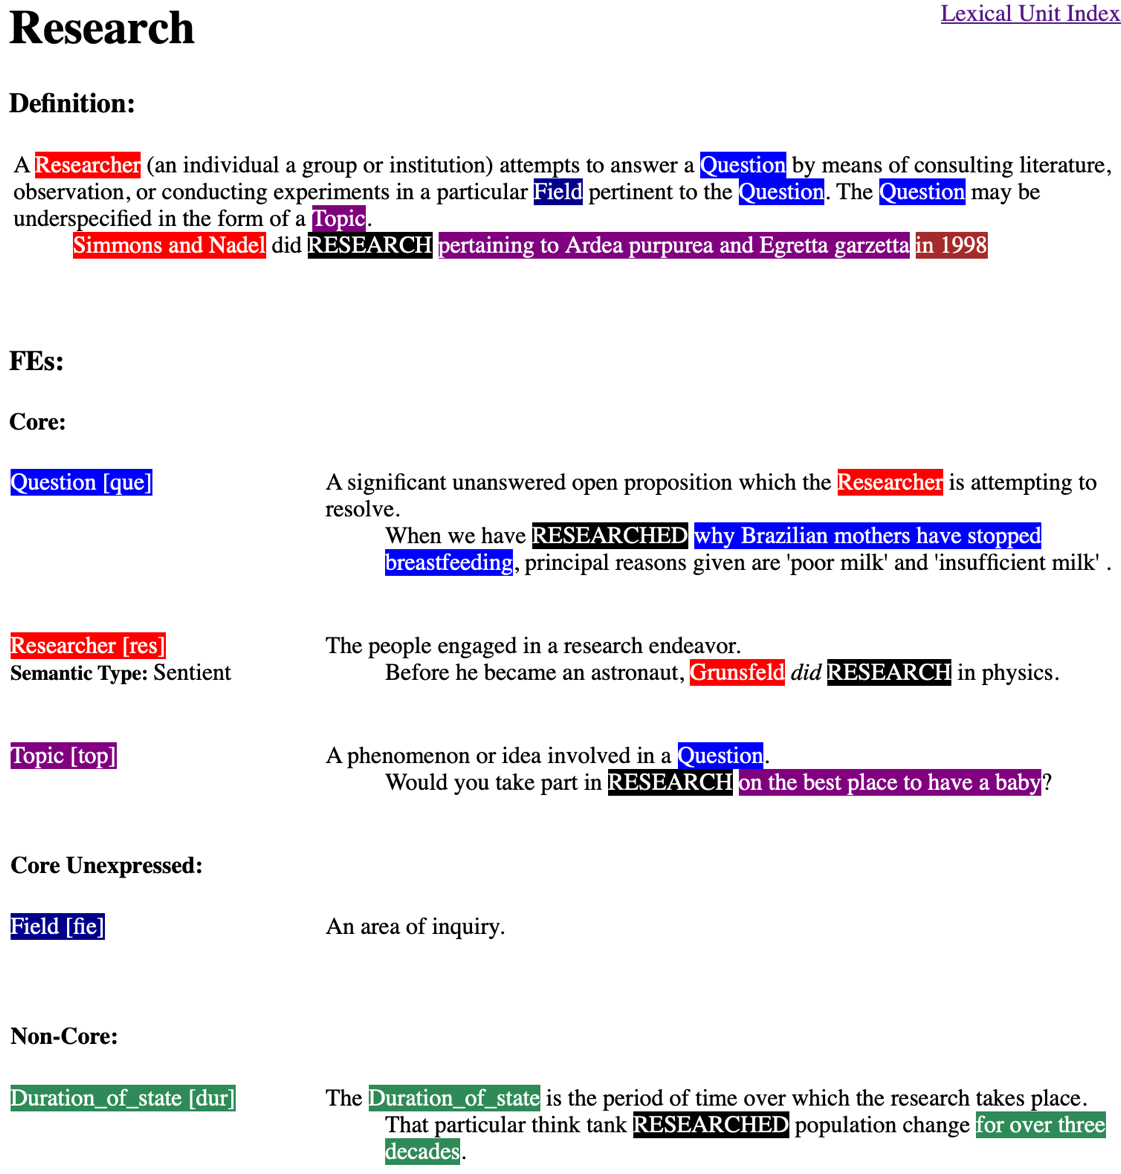
\includegraphics[width=\textwidth]{figures/media/image2.png}
  \caption{\label{fig:framenet-research}Ausschnitt aus dem \FN{Research}-Frame im Berkeley \emph{FrameNet} (Definition und ein Teil der FE).}
\end{figure}

Ersichtlich ist, dass der Frame aus den Kern-FE \textsc{question}, \textsc{researcher}, \textsc{topic}, sowie dem \emph{Core Unexpressed}\footnote{Als \emph{Core Unexpressed} werden solche FE annotiert, die zwar zu den Core-FE zählen, jedoch in Nachkommen des Frames nicht mehr explizit realisiert werden \autocite[24-25]{ruppenhoferFrameNetIIExtended2016}.} FE \textsc{field} besteht. Als \emph{Non-Core}-FE werden des Weiteren \textsc{duration\_of\_state}, \textsc{manner}, \textsc{means}, \textsc{place}, \textsc{population}, \textsc{purpose}, \textsc{time} und \textsc{type} gelistet. Eine kurze Definition und i.d.R. ein Beispielsatz geben des Weiteren Auskunft über die Rolle, die die jeweiligen FE im Gesamt-Frame spielen. Deutlich wird an dieser Stelle die Orientierung der Fillmoreschen Frame-Semantik an der Valenzgrammatik. So entsprechen die \emph{Core}-FE i.d.R. den Komplementen bzw. Ergänzungen des Verbs und die \emph{Non-Core}-FE seinen Supplementen bzw. Angaben.\footnote{Findet sich für ein \emph{Core}-FE keine lexikalische Realisierung, wird dies als ‚Nullinstantiierung` annotiert \autocite[28]{ruppenhoferFrameNetIIExtended2016}.} Es wird für den Frame des Weiteren angegeben, dass sich die FE \textsc{field}, \textsc{question} und \textsc{topic} in einem FE-\emph{CoreSet} zusammenfassen lassen, von ihnen also i.d.R. nur eines realisiert wird \autocite[25-26]{ruppenhoferFrameNetIIExtended2016}. Als LE, d.\,h. frame-evozierende Lexeme, sind ihm \emph{investigate.v, research.n} und \emph{research.v} zugeordnet. Eine LE stellt dabei immer ein Wort-Frame-Paar dar, sodass im Falle polysemer oder homonymer Wörter ein Wort auch mehreren Frames zugeordnet sein kann, es also mehrere gleichlautende LE geben kann. Eine gewisse Disambiguierung leisten darüber hinaus die den LE angefügten \emph{Part-of-Speech}-Tags (POS-Tags), die \emph{research} in diesem Frame ein Mal als Nomen und ein Mal als Verb ausweisen. Im Frame-Eintrag sind außerdem Frame-zu-Frame-Relationen vermerkt; in diesem Fall, dass der Frame seine Struktur bzw. Semantik vom \FN{Scrutiny}-Frame erbt und wiederum an den \FN{Trying\_out}-Frame vererbt. Die Idee ist dabei, dass „each semantic fact about the parent must correspond to an equally specific or more specific fact about the child'' \autocite[80]{ruppenhoferFrameNetIIExtended2016}. In diesem Sinne lassen sich teils übereinstimmende FE identifizieren, auch wenn die FE des Kind-Frames häufig semantisch differenzierter sind. Weiterhin wird der \FN{Cogitation}-Frame unter „Uses:`` angegeben, was einer „reference in a very general kind of way to the structure of a more abstract, schematic frame`` entspricht und insbesondere für Fälle genutzt werden soll, in denen ein Teil der durch den Kind-Frame aufgerufenen Szene auf den Eltern-Frame Bezug nimmt \autocite[83]{ruppenhoferFrameNetIIExtended2016}. \figref{fig:framegrapher-research} zeigt die für Frames typische Visualisierung der Vernetzung des Frames in \emph{FrameNet} als Netzwerk-Graph:

\begin{figure}
  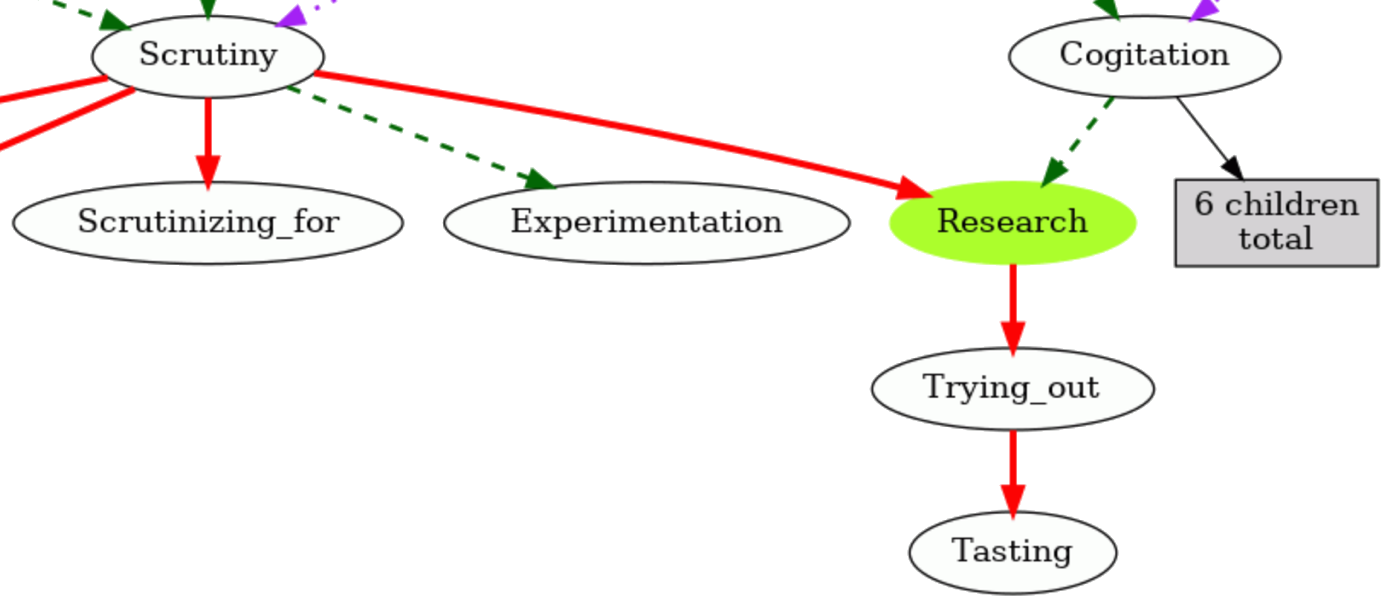
\includegraphics[width=\textwidth]{figures/media/image3.png}
  \caption{\label{fig:framegrapher-research}Ergebnis der Abfrage des \FN{Research}-Frames im \emph{FrameGrapher}-Tool in \emph{FrameNet} (\emph{maximum number of generations}: 2, \emph{maximum number of peripheral children}: 5).}
\end{figure}

\subsubsubsection{Erstellungsprozess eines Frame-Eintrags}\label{erstellungsprozess-eines-frame-eintrags}

Die Erstellung eines \emph{FrameNet}-Frames lässt sich wie folgt gliedern: Ausgangspunkt ist der Eindruck der Annotator*innen, dass einer Gruppe von Wörtern ein oder mehrere gemeinsame Frames unterliegen könnte. Dieser Eindruck wird sodann anhand von Korpusevidenz näher geprüft und es werden aus den LE ein oder mehrere Frames erstellt \autocite[11]{ruppenhoferFrameNetIIExtended2016}. Als Anforderung für den gemeinsamen semantischen Nenner von Wörtern können dabei die folgenden, den situativ-szenischen Charakter von Frames addressierenden Kriterien gelten: „a background of the kinds of questions they answer, the kinds of situations that are presupposed for sentences with the target, and the way that a speaker is thinking about a situation when they use the target'' \autocite[11]{ruppenhoferFrameNetIIExtended2016}. Sie sollen darüber hinaus insbesondere die gleiche Anzahl und Art von FE aufweisen.\footnote{An dieser Anforderung wird noch einmal deutlich, dass \emph{FrameNet}-Frames sehr eng an valenztheoretischen Ideen ausgerichtet ist, denn scheinbar lassen sich FE schon unabhängig von Frames für einzelne Wörter bestimmen.} Welche Methoden bei der Sammlung von LE, die zu einem Frame gehören, zum Einsatz kommen, bzw. ob dabei überhaupt ein systematisches methodisches Vorgehen angewandt wird, bleibt allerdings offen.

\subsubsubsection{Welche Frames werden aufgenommen?}\label{welche-frames-werden-aufgenommen}

\emph{FrameNet} ist insgesamt eher einem lexikographischen Zugang verpflichtet als einem, der ein wirklich breites semantisches Wissen, wie Fillmore es noch in der \emph{Understanding-Semantics}-Phase gefordert hatte, oder gar das ‚gesamte verstehensrelevante Wissen` im Sinne Busses einbeziehen würde. Selbst die Ebene des namensgebenden Frames rückt zugunsten der angezielten lexikalischen Ebene eher in den Hintergrund, wenn es in der Dokumentation zum Berkeley-\emph{FrameNet} heißt:

\begin{quote}
The Berkeley FrameNet project is creating an on-line lexical resource for English, based on \textbf{frame semantics} and supported by corpus evidence. The aim is to document the range of semantic and syntactic combinatory possibilities-- \textbf{valences}--of each word in each of its senses, through computer-assisted annotation of example sentences and automatic tabulation and display of the annotation results. \autocite[7]{ruppenhoferFrameNetIIExtended2016}
\end{quote}

Durch die Ausrichtung des Projektes auf Wortvalenzen ist außerdem ein recht starker Fokus auf Verben und deverbale Nominalisierungen zu konstatieren, was bereits durch Fillmore so angedacht ist. Dies hängt auch mit dem Konzept des „dominant frame`` \autocite[324]{fillmoreFramenetActionCase2003} zusammen, das die Autor*innen einführen, jedoch kaum näher erläutern. Nur in Ausnahmefällen, etwa bei Funktionsverbgefügen („support expressions``), könne ein Nomen den dominanten Frame eines Satzes evozieren:

\begin{quote}
Although in principle members of all major lexical categories can evoke a semantic frame, the dominant semantic frame of a sentence is usually evoked by the sentence's main verb. In some situations, however, it is a noun that provides the dominant frame; in fact, in certain styles of academic or political writing the dominant frame informing the meaning of the sentence is a noun \autocite[324]{fillmoreFramenetActionCase2003}.
\end{quote}

Auch in den aktuellen \emph{FrameNet}-Guidelines wird dies deutlich. Zwar wird Nomen generell ein Frame-evozierendes Potenzial zuerkannt, dieses sei bei Nomen, die Ereignisse oder Beziehungen bezeichnen, jedoch wesentlich ausgeprägter als etwa bei solchen, die Artefakte benennen \autocite[43]{ruppenhoferFrameNetIIExtended2016}. Dieser Maßgabe folgend, ist die Annotation von Frames an Nomen, die etwa Artefakte bezeichnen, noch immer die Ausnahme in \emph{FrameNet}. Ihnen wird zwar eine „minimal frame structure of their own`` \autocite[8]{ruppenhoferFrameNetIIExtended2016} zugesprochen, sie sollten jedoch vornehmlich als FE annotiert werden. Die Autor*innen gehen sogar so weit, dass die Annotation von Artefakt-bezeichnenden Nomen nur ein Mittel sein könne, um die Verben auffindbar zu machen, die diese Sätzen eigentlich regieren \autocite[8, siehe auch 51-52]{ruppenhoferFrameNetIIExtended2016}.

Neben der wortartbasierten Auswahl von Frames stellt auch die Frage der Granularität einen Aspekt dar, der über die in \emph{FrameNet} enthaltenen Frames entscheidet. Er ist für eine Frame-lexikographische Ressource von überragender Wichtigkeit; Ruppenhofer et al. \autocite*[17]{ruppenhoferFrameNetIIExtended2016} bezeichnen ihn sogar als „the most fundamental question``. Dass es etwa keine unterschiedlichen Frames für ‚Essen` und ‚Trinken` gibt, die in der Frame-Hierarchie dem bereits vorhandenen \FN{Ingestion}-Frame untergeordnet sein könnten, begründen sie mit forschungspraktischen Limitationen \autocite[17]{ruppenhoferFrameNetIIExtended2016}. Insgesamt wird dieser zentrale Aspekt jedoch nur sehr kurz thematisiert und wirkt unterreflektiert -- insbesondere vor dem Hintergrund der bereits thematisierten scheinbar wenig systematischen Auswahl zu beschreibender Frames durch das Annotationsteam. Die tatsächliche Frame-Auswahl kann diesen Eindruck nicht völlig entkräften. Einerseits finden sich Frames, die auf relativ spezifische Situationen eingehen wie der \FN{Bail\_decision}-, der \FN{Knot\_creation\_scenario}- oder der \FN{Hunting\_success\_or\_-failure}-Frame. Andererseits sind geradezu fundamentale soziale Konzepte, ohne die eine Orientierung in gesellschaftlichen Diskursen der vergangenen Jahre kaum möglich ist, wie ‚Krieg`, ‚Frieden`, ‚Pandemie` oder eben ‚Extremismus` nicht enthalten. Eine mögliche Lösung wäre es hier, auf semantisch ähnliche Frames wie \FN{Terrorism} statt ‚Extremismus` oder \FN{Hostile\_encounter} statt ‚Krieg` zurückzugreifen. Alternativ könnten auch semantisch sehr vage Frames wie der \FN{Catastrophe}-Frame, der als „\textsc{undesirable\_event} which affects the \textsc{patient} negatively``\footnote{\url{https://framenet.icsi.berkeley.edu/frameIndex}} definiert ist, genutzt werden. Als weitere Strategie zum Umgang mit diesem Problem wird die Definition neuer, an \emph{FrameNet} orientierter Frames vorgeschlagen und praktiziert \autocites[etwa bei][]{scholzVokabularImDiskurshistorischen2015, dutraBuildingFrameSemanticModel2023, bisiadaMeTooDreiSprachen2023}.

\subsection{Das Frame-Konzept Dietrich Busses}\label{das-frame-konzept-dietrich-busses}

\subsubsection{Überblick}\label{ueberblick}

In diesem Kapitel möchte ich das von Dietrich Busse im Rahmen seines Kompendiums zur Frame-Semantik \autocite*{busseFrameSemantikKompendium2012} entwickelte Frame-semantische Arbeitsmodell vorstellen. Das Modell kann als eine Zusammenführung und Erweiterung verschiedener Slot-Filler-Frame-Modelle begriffen werden. Besonderen Einfluss haben dabei die Arbeiten Bartletts, Fillmores, Minskys, Schank und Abelsons, Barsalous sowie die einiger germanistischer Linguist*innen, darunter Konerding, Lönneker-Rodman, Klein und Ziem. Das folgende Zitat fasst Status, Wesen und Funktion von Frames im Sinne Busses zusammen:

\begin{quote}
Ein Frame bezieht sich auf ein „Etwas``, das erst durch die „Attribute`` des Frames, denen jeweils bestimmte „Werte`` zugewiesen werden müssen, als dieses Etwas bestimmt, d.\,h. als ein aus dem Kontinuum der zunächst ungeschiedenen Sinnesdaten heraushebbares „Etwas`` ausgegrenzt wird. D.\,h.: Erst dadurch, dass ihm Eigenschaften (via Attribute) zugeschrieben werden, wird es als etwas Identisches kognitiv bzw. epistemisch „greifbar``, bekommt eine Identität, die es überhaupt erst zu einem wiederholt referierbaren „Etwas`` machen. Die „Kategorie`` in Barsalous Sinne (die dann im Sinne Lönnekers mit einem „Frame-Namen`` benannt wird) ist also zunächst nichts anders als eine abstrakte (epistemisch „leere``) Position im Sinne eines „hier gibt es ein Etwas``. Erst durch die Spezifikation von konkreten Merkmalen, Eigenschaften, die dieses „Etwas`` von anderen „Etwassen`` abzugrenzen erlauben, im Sinne der Attribute Barsalous, bekommt dieses „Etwas`` eine konkrete, mit Informationen gefüllte, und auch erst dann wiedererkennbare Gestalt. „Wiedererkennbar`` meint dann, dass mit dem „Datenset``, der den Frame ausmacht, neue Wahrnehmungssituationen (oder epistemische Konfigurationen) kognitiv verarbeitet werden, so dass sie als „Exemplare`` des Frames identifiziert werden können. Ein „allgemeiner`` Frame ist dann so etwas wie eine Datenstruktur, gemeint als abstrakte „Suchstruktur``, die im kognitiven (epistemischen) Prozess der Identifizierung von Entitäten (als Entitäten eines bestimmten Typs) angewendet wird. Die konkrete Datenstruktur im Kontinuum der Sinnesdaten bzw. kognitiven Konfigurationen, die durch die Aufprägung der abstrakten Struktur ausgegrenzt wird, ist dann ein „Exemplar`` dieses Frames. \autocite[589]{busseFrameSemantikKompendium2012}
\end{quote}

In diesem Zitat werden mehrere Wesensmerkmale von Frames im Sinne Busses deutlich:

\begin{enumerate}
\def\labelenumi{\arabic{enumi})}
\item
  Frames sind epistemische Entitäten, die es ermöglichen, eingehende „Sinnesdaten`` zu verarbeiten und in dem Sinne zu ordnen, dass sie als etwas Zusammengehöriges wahrgenommen werden, ihnen eine „Identität`` zugeschrieben wird und sie somit als „Etwas`` erkennbar sind. Die Wiedererkennbarkeit und der epistemische Gehalt wird durch die Zuschreibung von Eigenschaften über Attribute geleistet; die Referenzierbarkeit über einen Frame-Namen. Es wird hier auch der konstruktivistische Charakter von Frames deutlich: Gegenstände werden erst in der Verarbeitung von Eindrücken konstituiert und sind nicht einfach ‚da`.
\item
  In diesen Verarbeitungsprozessen geht es insbesondere um die musterbasierte Wiedererkenneung bzw. Identifizierung von Frames. Sie finden ausdrücklich auf einer kognitiven Ebene statt. Auf die Rolle dieser mit dem Frame-Konzept verbundenen und nicht unumstrittenen Festlegung wird in \chapref{frames-und-kognition} noch näher eingegangen.
\item
  Es werden zudem verschiedene Ebenen oder Zustände von Frames beschrieben. Zu unterscheiden ist dabei u.\,a. zwischen den kognitiven, schablonenartigen Datenstrukturen, die zur Einordnung von Sinnesdaten herangezogen werden und den Daten selbst, die mithilfe dieser Struktur als passend zur Schablone identifiziert werden. Mit diesem Aspekt wird sich das folgende Kapitel auseinandersetzen.
\end{enumerate}

\subsubsection{Type- und Token-Frames}\label{type--und-token-frames}

Busse bleibt nicht bei dieser Beschreibung verschiedener eher prozesshafter Frame-Zustände, sondern differenziert Frames nach insgesamt fünf (hier nicht im Detail aufgeführten) Ebenen und mithilfe der folgenden drei Kriterien: dem Muster- bzw. Exemplarcharakter der Frames (Type- vs. Token-Frames), der Art von Wissen, die sie organisieren (soziales vs. individuelles Wissen) und ihrem kognitiven Status bei der Wissensrealisierung (allgemeine Frames vs. konkret im individuellen Kurzzeitgedächtnis instantiierte Frames). Besonders relevant und von Busse immer wieder hervorgehoben ist die Unterscheidung von Type- und Token-Frames, verstanden als „die Differenz zwischen einem abstrakten Muster und seiner konkreten Anwendung / Realisierung / Konkretisierung / Aktualisierung`` \autocite*[614]{busseFrameSemantikKompendium2012}. Unter einem Type-Frame ist also ein schablonenhafter Frame zu verstehen, dessen Slots offen oder nur mit Default-Werten befüllt sind und der als bestehendes Muster dazu dient, Sinneseindrücke einzuordnen. Token-Frames hingegen sind Realisierungen der Type-Frames und insofern mit konkreten Daten gefüllt und entsprechend darzustellen \autocite[539]{busseFrameSemantikKompendium2012}.

Es lassen sich des Weiteren Frames des individuellen kognitiven Wissens von solchen des sozialen Wissens unterscheiden. Für die spätere Operationalisierung und Methodenentwicklung ist relevant, dass die individuellen, kognitiven Frames nicht unmittelbar zugänglich sind, sondern nur interpretativ „auf der Grundlage von sprachlichen, ko-textuellen, kontextuellen und situativen Daten sowie ‚Hintergrundwissen`\,`` \autocite[538]{busseFrameSemantikKompendium2012} rekonstruiert werden können. In Hinblick auf die Erschließbarkeit von Token- und Type-Frames ist davon auszugehen, dass die Instantiierung von Token-Frames in einer konstitutiven Wechselwirkung mit den musterhaften Type-Frames steht, letztere mithin in einem Abstraktionsschritt aus der Menge der rekonstruierten Token-Frames ermittelt werden können. Aufgrund der Rekursivität von Frames ist allerdings davon auszugehen, dass „solche Beschreibungen eher komplexen Frame-Vernetzungen als isolierten Einzel-Frames entsprechen`` \autocite[538]{busseFrameSemantikKompendium2012}.

\subsubsection{Frame-Struktur: Slots, Filler und Relationen}\label{frame-struktur-slots-filler-und-relationen}

Wie Fillmore, Minsky und Barsalou entwirft auch Busse ein Frame-Modell, das aus einem Frame-Kern und einer Slot-Filler-Struktur besteht, wobei der Frame-Kern eher eine benennende als eine epistemisch spezifizierende Funktion hat, indem er „markiert, dass es hier ein (epistemisches) ‚Etwas` gibt, auf das sich die nachfolgend spezifizierten Frame-Elemente, Relationen und Aspekte beziehen`` \autocite[731]{busseFrameSemantikKompendium2012}. Die Filler der Slots stellen jeweils selbst Frames dar, sodass man, wie auch bei Minsky und dann insbesondere bei Barsalou,\footnote{So heißt es bei Barsalou „Knowledge appears to be frames all the way down, with every component of a frame potentially decomposing recursively into a more specific frame.`` \autocite*[41]{barsalouFlexibilityStructureLinguistic1993}} von einem rekursiven Frame-Modell sprechen kann, das im Folgenden anhand einer Abbildung Busses (\figref{fig:maus-frame}) näher erläutert werden soll:

\begin{figure}
  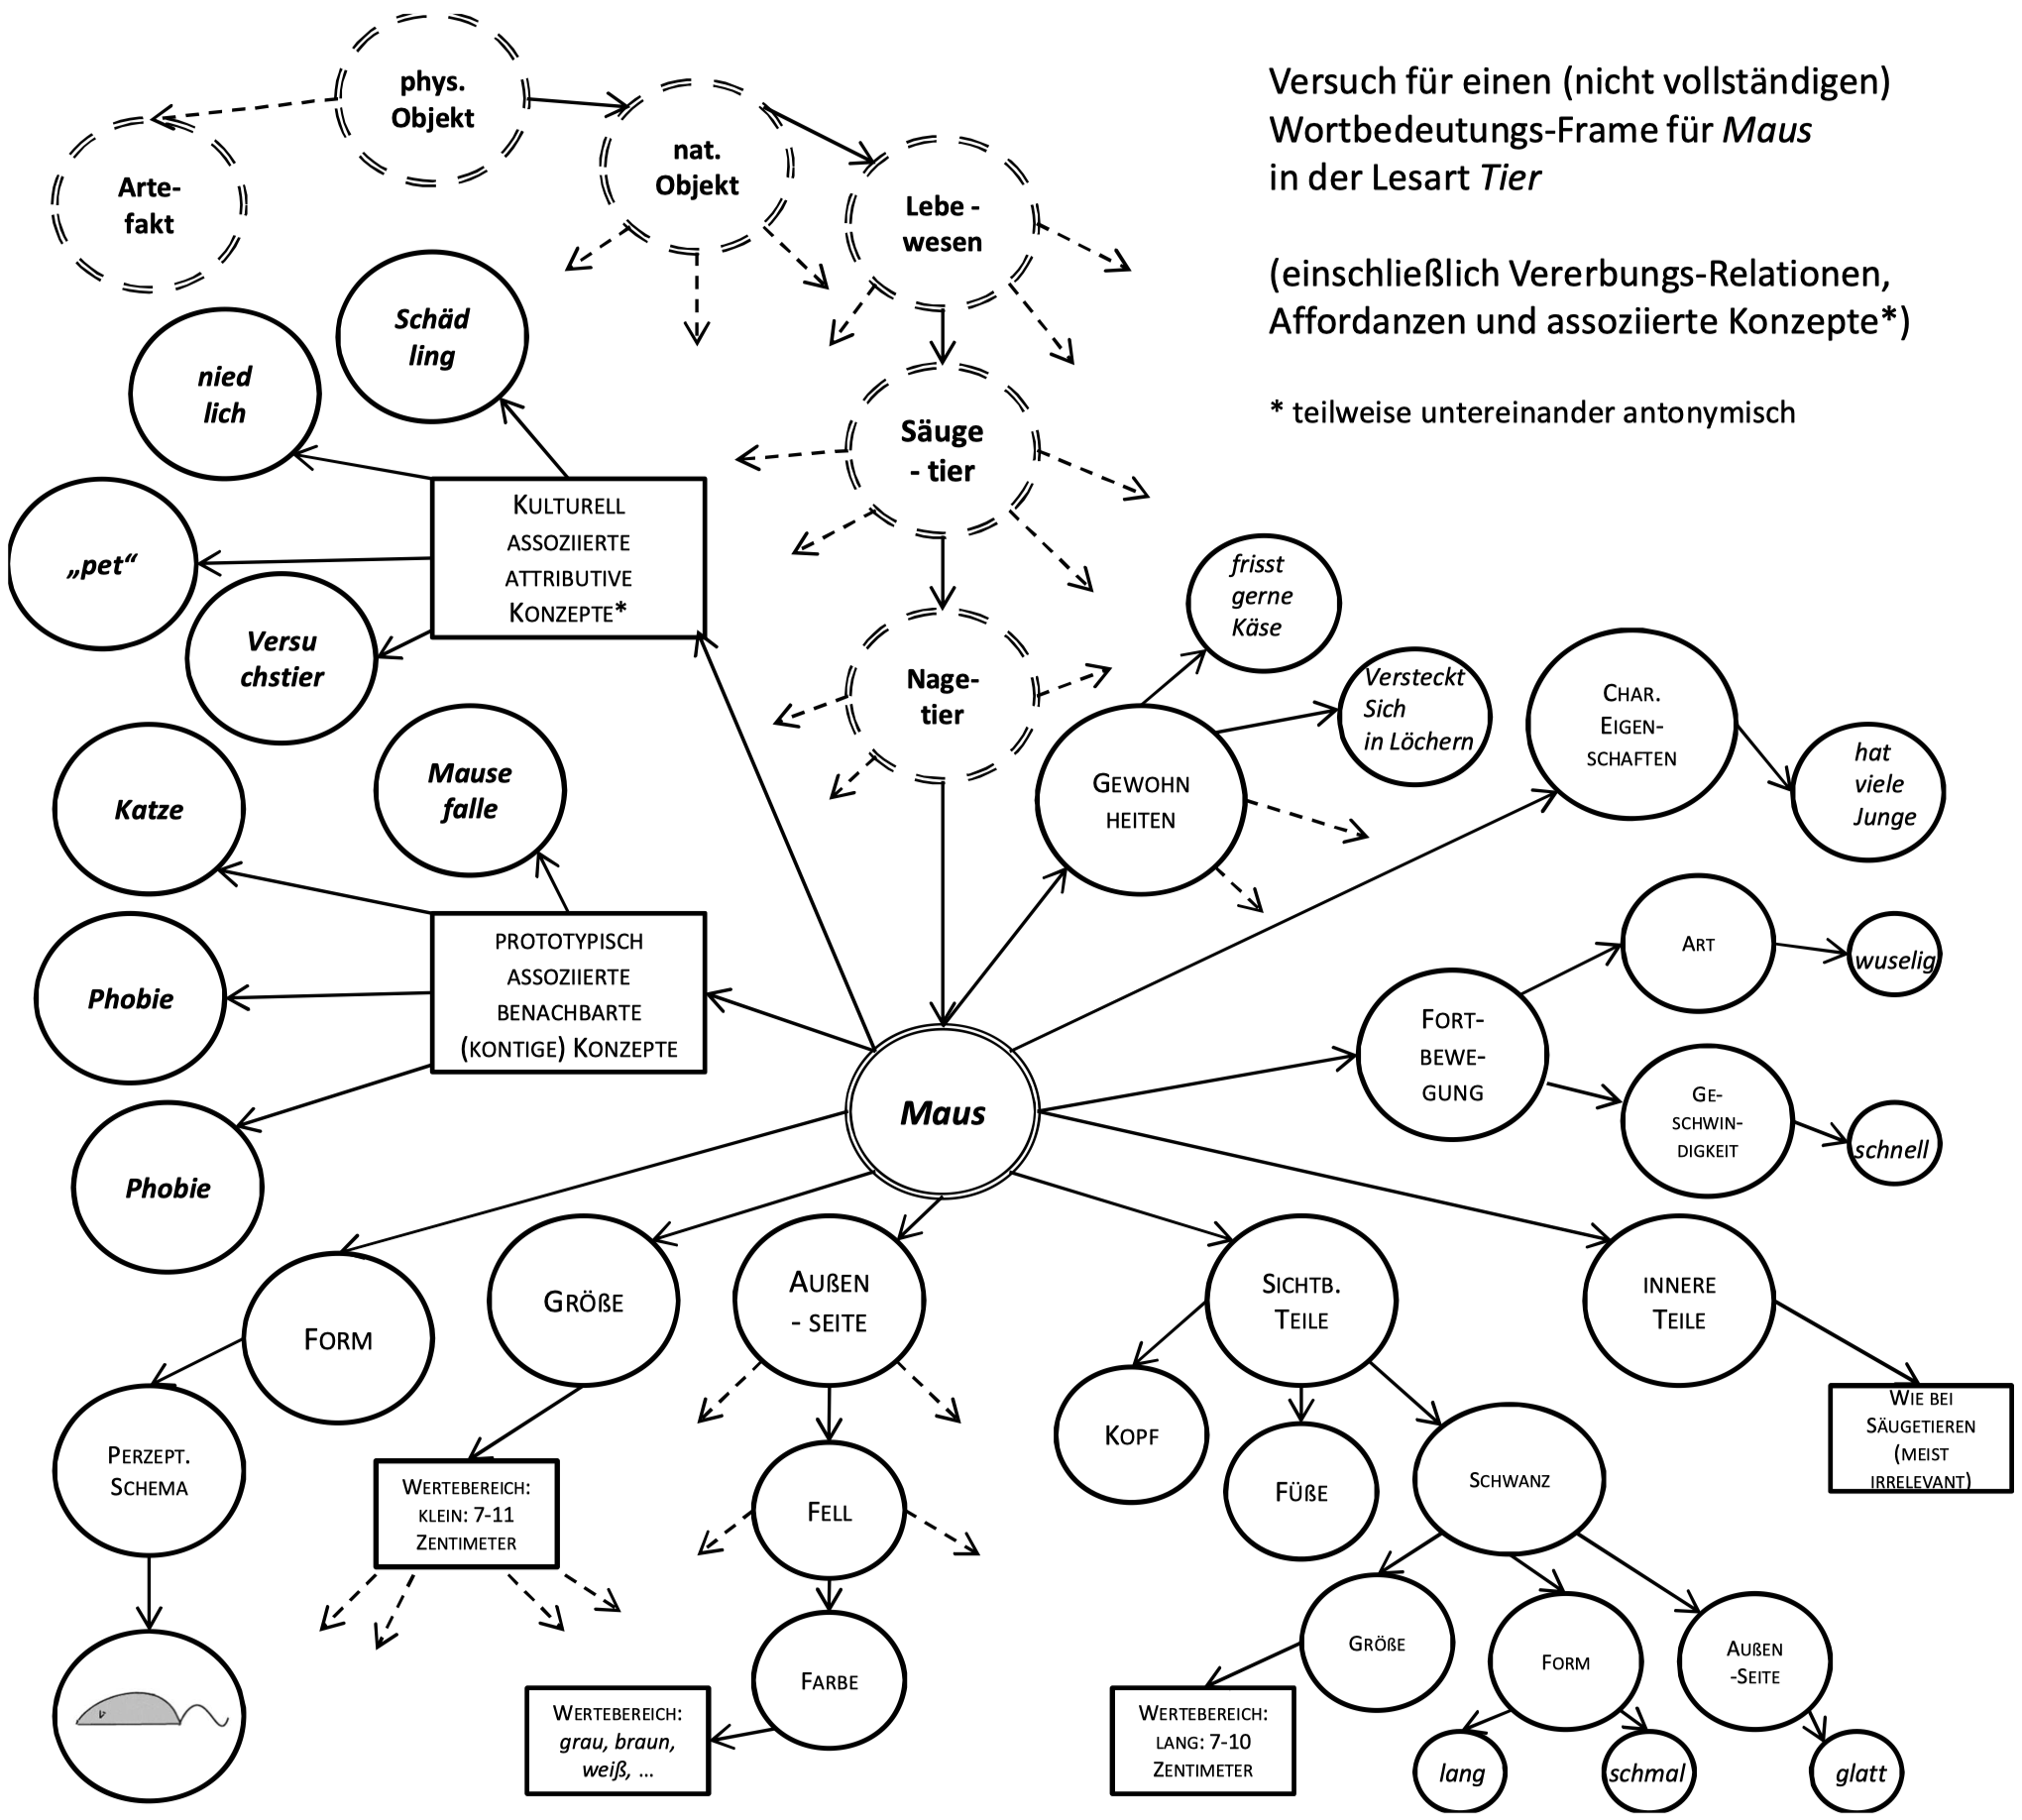
\includegraphics[width=\textwidth]{figures/media/image4.png}
  \caption{\label{fig:maus-frame}Entwurf eines Maus-Type-Frames (Abbildung 7-30 aus \citealt[744]{busseFrameSemantikKompendium2012}).}
\end{figure}

Es wird zunächst deutlich, dass der Maus-Frame selbst von einer Reihe übergeordneter Frames abstammt (Artefakt → phys. Objekt → nat. Objekt → Lebewesen → Säugetier → Nagetier). Slots und Filler sind in der Abbildung als Knoten angezeigt, während die Relationen zwischen ihnen als gerichtete Kanten (Pfeile) abgebildet werden. Alternative Relationen sind jeweils als gestrichelte, feste Relationen als durchgehende Pfeile dargestellt. Einzelne Werte sind nur in den Blättern des Baumes zu finden und durch einen den Text eng umschließenden Kreis verwirklicht. Werden keine konkreten Werte, sondern Wertebereiche angegeben, so geschieht dies in Form eines Vierecks. Während bei Token-Frames auch auf der untersten dargestellten Ebene die Filler der Slots angegeben werden, werden beim hier dargestellten Type-Frame Wertebereiche notiert, in denen sich die Filler typischerweise bewegen sowie der Typ des Wertebereichs und ggf. eine Information dazu, inwiefern eine konkrete Füllung des Slots oder ein Default-Wert\footnote{Das Konzept des Default-Wertes -- dass also nicht jedes Wissenselement sprachlich explizit gemacht werden muss und dennoch als mit einem bestimmten Wert belegt mitverstanden wird -- gibt es bereits bei Minsky; es wird aber insbesondere von Ziem \autocite*{ziemFramesUndSprachliches2008} als für die Frame-Semantik zentral herausgestellt. Er bezeichnet sie auch als „{[}i{]}mplizite Prädikationen``, die seines Erachtens den „weitaus größt{[}en{]} Teil verstehensrelevanten Wissens`` in Texten ausmachen \autocite[335]{ziemFramesUndSprachliches2008}} zu erwarten ist \autocite[731-732]{busseFrameSemantikKompendium2012}. So wird etwa für den Slot ‚Farbe` der offene Wertebereich „grau, braun, weiß, ...`` angegeben. Auch assoziative attributive und benachbarte Konzepte werden -- ebenfalls durch ein Viereck gruppiert -- in die Frame-Darstellung aufgenommen und ergänzen in diesem Beispiel die ansonsten weitestgehend enzyklopädischen Daten durch eher kulturbezogene Aspekte.

Busse beschreibt darüber hinaus Relationen zwischen Frame-Elementen, die nicht auf Vererbungs- bzw. Slot-Filler-Relationen zurückgehen, sondern das gemeinsame Auftreten von Frame-Elementen steuern:

\begin{quote}
In Frames bestehen zusätzlich zu den Typen von Relationen, die Anschlussstellen (Slots, Attribute) den Frame-Kernen, sowie Zuschreibungen (Filler, Werte) den Anschlussstellen (den jeweiligen Slots) zuordnen, weitere zentrale, teilweise ebenfalls Frame-definierende Typen von Relationen, die einzelne Frame-Elemente (Anschlussstellen / Slots / Attribute und / oder Zuschreibungen / Filler / Werte) untereinander korrelieren, sie zu Frame-spezifischen Gruppen von Frame-Elementen zusammenfassen, die immer gemeinsam vorkommen müssen, oder sachlich zwingende Kovarianzen (bzw. Abhängigkeits-Relationen) zwischen einzelnen Zuschreibungen (Fillern, Werten) festlegen. Diese Relationen (Korrelationen, Kovarianzen) wirken als die Variabilität der Frame-Struktur einschränkende Bedingungen (Restriktionen, Beschränkungen), die entweder bestimmte Frame-Elemente (beim Auftreten anderer korrelierter Frame-Elemente) erzwingen (konstruktive Korrelationen), oder das Auftreten bestimmter Frame-Elemente (z.\,B. Filler, Werte) zu bestimmten Anschlussstellen in Kovarianz mit bestimmten anderen Frame-Elementen (Fillern, Werten) zu bestimmten anderen Anschlussstellen auf einen bestimmten Bereich beschränken (restriktive Korrelationen). \autocite[570-571]{busseFrameSemantikKompendium2012}
\end{quote}
\largerpage
Er untergliedert diese „\emph{Relationen zwischen Attributen gleichen Typs}`` in ‚Gruppen von Attributen`, ‚Strukturelle Invarianten` und ‚Attribut-Constraints`. Erstere können entweder statistisch-usuell bestimmt werden als „bestimmte festere Ko-Okkurenzen von Slots bzw. Attributen`` oder als „inhaltlich spezifizierte und zusammenhängende Gruppen (die sich dann nur enzyklopädisch beschreiben / definieren bzw. abgrenzen lassen)`` \autocite[594]{busseFrameSemantikKompendium2012}, womit etwa die auf das Aussehen der Maus bezogenen FE wie \textsc{Form}, \textsc{Größe} oder \textsc{Außenseite} gruppiert werden könnten. Darüber hinaus sei auch eine funktionale Bestimmung der Attributgruppen möglich, etwa nach (vor allem bei verbal geprägten Frames relevanten) Aktanten- und (vor allem bei nominal geprägten Frames relevanten) Eigenschafts-FE. Den Begriff der ‚strukturellen Invariante` übernimmt Busse von Barsalou, der damit feste, notwendige Beziehungen zwischen FE bezeichnet, die etwa räumlicher oder zeitlicher Natur sein können. Als Beispiel für erstere nennt Busse die Relation zwischen Sitz und Lehne bei einem Stuhl, für zweitere die Relation zwischen Essen und Bezahlen \autocite*[565]{busseFrameSemantikKompendium2012}. Auch in Bezug auf Wertebereiche spielen strukturelle Invarianten eine Rolle, indem sie für bestimmte Wertebereiche eine quasi absolute Grenze setzen, bei deren Überschreitung nicht mehr von einer Extension des Wertebereiches um einen vielleicht ungewöhnlichen Wert ausgegangen werden kann. Der Begriff \emph{constraint} letztlich wird ebenfalls von Barsalou übernommen. Hiermit sind Wechselwirkungen zwischen den FE gemeint, die anders als bei den strukturellen Invarianten nicht als „normativ{[}e{]} Wahrheiten`` zu fassen sind, sondern eher eine „‚systematische Variabilität` zwischen den Werten von Attributen {[}herstellen{]}`` und darüber hinaus häufig auf Alltagswissen beruhen \autocite[566]{busseFrameSemantikKompendium2012}. Als Beispiele führt Busse an, dass ‚Mallorca` als Filler für den Slot \textsc{Ort} in einem Urlaub-Frame bestimmte Filler für den Slot \textsc{Urlaubsaktivität} nahelegt (etwa ‚surfen`), während andere Filler wie ‚skifahren` nur bei anderen Urlaubsorten zu erwarten sind. Solche Constraints können sowohl zwischen Slots als auch Fillern auftreten.

\subsubsection{Sprachoberflächliche Bezugspunkte}\label{sprachoberflaechliche-bezugspunkte}
\largerpage
Für eine diskurslinguistische Arbeit sind Frames als Strukturen epistemischen Wissens insbesondere unter Berücksichtigung ihrer sprachlichen Repräsentation von Interesse. Es geht also darum, wie von Texten überhaupt auf Frames geschlossen werden kann oder auch wie Frames Texte und Texte Frames formen. Die Frame-Theoretiker entwerfen dieses Verhältnis jeweils unterschiedlich, wobei die lexikalische Ebene i.d.R. den primären Bezugspunkt darstellt. Für Busse stellt die „adäquate Analyse der Beziehungen zwischen Lexemen und Frames`` die „wichtigste Aufgabe einer angewandten Frame-Forschung`` dar, wobei er seine eigenen Ausführungen als „erste tastende Vermutungen``, die weiterer Forschung und empirischer Validierung bedürfen, einordnet \autocite*[656]{busseFrameSemantikKompendium2012}. Im Folgenden möchte ich die in meinen Augen wichtigsten Aspekte seiner Überlegungen zusammenfassen, die vollständige Darstellung findet sich in Busse \autocite*[652-658 insb.]{busseFrameSemantikKompendium2012}

Als Frame-evozierendes sprachliches Zeichen stellt auch er das Lexem in den Fokus. Lexeme evozieren Frames und legen -- unter Umständen im Zusammenspiel mit anderen Lexemen des Kotextes -- Slots und Filler von Frames sowie eine bestimmte Perspektive fest \autocite[656-657]{busseFrameSemantikKompendium2012}. Die Zuordnung von Lexemen zu Frames ist dabei jedoch nie starr; stattdessen hebt Busse Minskys Idee eines probabilistischen \emph{matching process} hervor:

\begin{quote}
Laut Minsky gleicht das Wort-Verstehen eher einem Abgleich-Prozess (matching process), bei dem möglicherweise mehrere Frames durchlaufen werden, bevor der passende aktiviert und herausgefunden ist. Verstehen von Wörtern wird damit zu einem \emph{probabilistischen} Unterfangen, das auf Plausibilitäten und Wahrscheinlichkeiten eher beruht als auf eindeutigen Gewissheiten. \autocite[653]{busseFrameSemantikKompendium2012}
\end{quote}

Dazu passt auch, dass Lexeme in Busses Frame-Entwurf „mehr als einen Frame parallel evozieren`` oder mehrere Lexeme den gleichen Frame evozieren können \autocite[657]{busseFrameSemantikKompendium2012}. Höchst interessant für die vorliegende Arbeit ist, dass er die Bedeutung wesentlicher kontextualistischer Konzepte hervorhebt, die insbesondere im Rahmen korpuslinguistischer Theoriebildung eine herausragende Rolle gespielt haben (siehe \chapref{distributionelle-semantik-korpuspragmatik-und-das-corpus-driven-paradigma}). Dazu zählt insbesondere die Kontextualisierungsleistung von Kollokationen, die für ihn darin besteht, andere Frames anzuschließen und einen Frame mithin semantisch zu spezifizieren: „Lexeme kontextualisieren Frames, indem sie sie in Kollokationen und Syntagmen einbetten und dadurch Beziehungen zu anderen Frames nahelegen.`` \autocite[656]{busseFrameSemantikKompendium2012}. Busse konstatiert zur Bedeutung von Kollokationen des Weiteren einen Zusammenhang, den bereits Minsky hervorgehoben hat, nämlich dass Frames mitunter nicht durch ein einzelnes Lexem, sondern durch das Zusammenspiel verschiedener Lexeme evoziert werden. So zitiert Minsky ein Beispiel aus Charniak \autocite*{charniakModelChildrensStory1972}, in dem das Szenario beschrieben wird, dass ein Kind einem anderen einen Drachen schenken möchte, jedoch nicht das nötige Geld dafür hat:

\begin{quote}
She wondered if he would like a kite. She went to her room and shook her piggy bank. It made no sound. \autocite[Charniak 1972 in][35]{minskyFrameworkRepresentingKnowledge1974}
\end{quote}

Obwohl in dem Szenario nicht explizit von (keinem) Geld, einem Kind oder einem Geschenk die Rede ist, werden die entsprechenden Frames durch die syntagmatische Kombination der einzelnen Wörter evoziert. Es wird also deutlich -- und das ist für einen korpuslinguistischen Zugang von höchstem Interesse -- dass auch syntagmatische Lexemkombinationen, korpuslinguistisch gesprochen: Kollokationen, für die Frame-Evokation von Bedeutung sind. Sie evozieren zum einen mehrere für das Verständnis relevante Frames, zum anderen sorgen sie dafür, dass die einzelnen Frames zueinander kompatibel ausgewählt werden:

\begin{quote}
Lexem-Kombinationen und Lexem-Ketten evozieren Frame-theoretisch gesehen einerseits Kombinationen von Frames, andererseits führt die Kombination von Lexemen dazu, dass in einem Abgleich-Prozess (matching process im Sinne von Minsky) die ausdrucksseitige Präsenz von zwei oder mehreren Lexemen die Evokation der Lexem-induzierten Frames wechselseitig adaptiv beeinflusst, genauer: die evozierten Frames an den durch die Kombination signalisierten epistemischen Kontext anpasst und ggf. irrtümliche erste (durch isolierte Lexem-Verarbeitung induzierte) Frame-Evokationen korrigiert. \autocite[660]{busseFrameSemantikKompendium2012}
\end{quote}

Ein weiteres Konzept, das der Korpuslinguistik entstammt und das Busse für relevant für die Beschreibung hält, ist das der semantischen Prosodie. Er referiert hier auf die Arbeiten der Korpuslinguisten Louw \autocite*{louwIronyTextInsincerity1993} und Stubbs \autocite*{stubbsTextCorpusAnalysis1996},\footnote{Wie Louw \autocite*[31-32]{louwIronyTextInsincerity1993} hervorhebt, geht der Begriff allerdings ursprünglich auf John Sinclair zurück.} die das Phänomen beschreiben, dass

\begin{quote}
lexikalische Wahlen oft starke Erwartungen dessen „was als nächstes kommt`` wecken. Es handelt sich bei diesem bisher kaum beschriebenen Phänomen um typische Kollokationen von Bezugswörtern mit anderen Wörtern, denen insgesamt eine semantische Tendenz der Verwendung der Bezugswörter zugrunde liegt mit dem Effekt, dass, wenn immer das Bezugswort verwendet wird, nur bestimmte Kollokate (mit einer bestimmten semantischen Tendenz) erwartet werden, auch wenn andere logisch genau so möglich wären. M.a.W., es geht um die „Präferenz`` von Lexemen, „sich mit einer ganzen semantischen Klasse von verbundenen Wörtern zu verbinden``, die dann ebenfalls wieder Frames und epistemische Kontexte evozieren. \autocite[655]{busseFrameSemantikKompendium2012}\footnote{Was Busse hier in Hinblick auf semantische Prosodie, also die semantische Färbung von Kollokaten, anspricht, ist nur ein Teilphänomen der von Sinclair beschriebenen Prinzipien der \emph{co-selection} bzw. des \emph{idiom principles} (siehe \chapref{der-corpus-driven-ansatz}), die für die Frame-semantische Modellierung genauso zu berücksichtigen wären.}
\end{quote}

Es ist also zu konstatieren, dass (sprachliche) Kontexte einen ganz wesentlichen Beitrag dazu liefern, einzelne Lexeme verstehen zu können, bzw. diese oft überhaupt erst im Verbund verständlich sind. Busse führt dazu auch die Positionen von Ballmer und Klein an, die diesen Punkt aus jeweils unterschiedlichen Positionen verdeutlichen: Während Ballmer den Fokus auf die Funktion von Sprachzeichen bei der Textproduktion legt, d.\,h. wie sie genutzt werden können, um bestimmte Kontexte im Wissen der Rezipient*innen aufzurufen, hebt Klein hervor, dass sich die Bedeutung sprachlicher Zeichen überhaupt nur in Bezug auf bestimmte Kontexte beschreiben lasse.

\subsubsection{Perspektivierung, Kontext und Frame-Wandel}\label{perspektivierung-kontext-und-frame-wandel}

In Busses Frame-Modell kann die Perspektivierung und Fokussierung eines Frames entweder durch die „Aktivierung bestimmter Sub-Sets von Slots / Attributen aus der Gesamt-Menge von Slots / Attributen eines \emph{type}-Frames`` oder durch die „Füllung der Slots mit spezifischen (Sets von) Werten`` geschehen \autocite[622]{busseFrameSemantikKompendium2012}. Dabei sei -- so Busses Arbeitshypothese -- die erste Variante typischer für Konkreta, die zweite für Abstrakta. Weiterhin relevant ist dabei, dass die nicht im Fokus bzw. Ausschnitt der Perspektive liegenden Teile des Frames weiterhin im Frame enthalten sind und referenzierbar bleiben:

\begin{quote}
Solche Perspektivierungen ändern jedoch nichts daran, dass in jeder Evozierung stets „der gesamte Frame präsent`` ist, wenn auch nicht in allen seinen epistemischen Elementen thematisch (oder im Aufmerksamkeitsfokus), doch als „Hintergrund``, eben „Kontext``, immer in seiner Gesamtheit „gegenwärtig`` (im Sinne von perspektivierbar, unmittelbar thematisierbar). \autocite[664]{busseFrameSemantikKompendium2012}
\end{quote}

Bedingt wird die Perspektivierung eines Frames bei Busse durch Ziele und Interessen, die er im Anschluss an Fillmore sowie die anderen von ihm betrachteten Frame-Theoretiker Minsky, Schank{\slash}Abelson und Barsalou in das Gebiet seiner Frame-Semantik einschließt \autocite*[620-621]{busseFrameSemantikKompendium2012}. Für den Rahmen dieser Arbeit besonders relevant ist dabei die Rolle für den Frame-Wandel, die er der Perspektivierung und Fokussierung sowie den sie leitenden „Ziel{[}en{]}, Interessen, Intentionen (und Zweck{[}en{]} und Funktionen)`` \autocite*[622]{busseFrameSemantikKompendium2012} bzw. rezipientenseitigen Erwartungen zuschreibt. Sie könnten sich nämlich „kognitiv oder sozial verfestigen und zu neuen \emph{type}-Frames (im individuellen oder gesellschaftlichen Wissen)`` bzw. zu „epistemisch verfestigt{[}en{]} Kontextualisierungen`` \autocite*[622]{busseFrameSemantikKompendium2012} führen. Die Rolle sprachlicher Zeichen ist dabei, dass sie die Perspektivierung bzw. Fokussierung leisten und -- sofern sich diese verfestigt -- zu „so etwas wie \emph{gesellschaftlich typisierte}{[}n{]} \emph{Perspektivierungen} und \emph{Fokussierungen} im Wissen`` \autocite[623]{busseFrameSemantikKompendium2012} führen. Zur Verfestigung von Slots bzw. Default-Werten von Slots rekurriert Busse außerdem auf Ziem \autocite*{ziemFramesUndSprachliches2008}, der mit Type- und Token-Frequenz zwei Formen von Verfestigung unterscheidet: Um eine hohe Type-Frequenz handelt es sich bei der Instanziierung eines Slots mit einer Vielzahl unterschiedlicher Token, während die wiederholte Instanziierung mit demselben Token eine hohe Token-Frequenz darstellt und zur Etablierung des Tokens als Default-Wert führt \autocite[627]{busseFrameSemantikKompendium2012}.

Sowohl in den Ausführungen zur sprachoberflächlichen Verankerung von Frames als auch zu ihrer epistemischen Perspektivierung ist bereits angeklungen, dass Ko- und Kontexte essenzieller Bestandteil einer angemessenen Frame-Modellierung sind und Einfluss auf Frames sowie die korrespondierenden sprachlichen Mittel haben. Bei Busse \emph{sind} Frames einerseits (epistemische) Kontexte, insofern sie einzelne Wissenselemente in größere Strukturen einbetten und somit kontextualisieren; er bezeichnet sie auch als „das Strukturformat für die verstehensrelevanten Wissens-Kontexte`` \autocite[664]{busseFrameSemantikKompendium2012}. Andererseits stellen Frames auch \emph{Mittel} der Kontextualisierung dar, insofern sie mittels der Verwendung einzelner sprachlicher Zeichen evoziert und perspektiviert werden. Gerade wenn Busse formuliert, dass Sprachzeichen „Kontextualisierungen ‚steuern`, insofern sie häufig bestimmte Perspektiven auf einen Wissenskomplex evozieren, d.\,h. bestimmte Aspekte eines Frame-Gefüges in den Vordergrund der Aufmerksamkeit und Relevanz rücken, andere im Hintergrund belassen``, \autocite[664]{busseFrameSemantikKompendium2012} wird außerdem eine inhaltliche Nähe zum Entmanschen Framing-Konzept deutlich (siehe \chapref{framing-in-den-kommunikationswissenschaften-bei-entman}). Interessanterweise nimmt Busse analog zum kontextuellen, wissensstrukturellen Charakter von Frames auch einen Kontextcharakter für Relationen sprachlicher Zeichen an. So stellen auch sie Kontexte dar, da sie in syntagmatischen und paradigmatischen Beziehungen zueinander stehen, was „in seiner Wichtigkeit und Wirkung unterschätzt`` \autocite[87]{busseDiskurslinguistikAlsKontextualisierung2007} werde. Gerade dass diese „eigen-kategorial{[}en{]}`` Relationen auf der Ebene der Sprachzeichen aufs engste mit ihren „fremd- oder kreuz-kategorial{[}en{]}`` \autocite[87]{busseDiskurslinguistikAlsKontextualisierung2007} Pendants auf der kognitiven Ebene, d.\,h. Frames, korrespondieren, liegt im Kerninteresse der vorliegenden Arbeit.

Die vielfältigen Kontextualisierungsmöglichkeiten, die sprachliche Zeichen bzw. Frames bieten, sind auch eng mit Aspekten des Frame-Wandels zusammenzudenken. Dieser wird von Busse als kontinuierlicher Prozess konzeptualisiert, der auf den einzelnen Token-Frame Instanziierungen im Diskurs beruht. Dadurch, dass Sprachteilnehmende Frames in der alltäglichen Kommunikation verwenden, wenn sie Äußerungen rezipieren oder produzieren, dabei immer wieder andere Slots und Filler wählen bzw. einem Frame zuordnen, verändern sich auch die Type-Frames. Es findet so, durch individuelle Äußerungen und über den Diskurs vermittelt, ständig Frame-Wandel statt:

\begin{quote}
In der individuellen Frame-Aktivierung schlagen sich die wechselhaften Positionen, Interessen, Ziele, Einstellungen, Perspektivierungen, Fokussierungen, Kontextualisierungen nieder, die dann teilweise (soweit sie „verbalisiert`` bzw. aus den sprachlich realisierten Texten sichtbar und nachvollziehbar sind) im gesellschaftlichen Diskurs „kommuniziert`` werden mit der möglichen Folge des „Aushandelns`` neuer Konventionen bzw. Strukturen der allgemeinen gesellschaftlich akzeptierten Frames (als Teil des „kulturellen Gedächtnisses``). Hat sich ein solcher Prozess der sozialen Verbreitung und Etablierung veränderter Frames vollzogen, hat ein diachroner Frame-Wandel stattgefunden, der dann entsprechend auch im individuellen Wissen einen Niederschlag finden kann. \autocite[627]{busseFrameSemantikKompendium2012}
\end{quote}

Diesen kontinuierlichen Wandelprozess, bei dem Frames kaum jemals plötzlich neu entstehen, sondern auf Anpassungen vorheriger Frames beruhen, bezeichnet Busse an gleicher Stelle auch als „Frame-Emergenz``. Dass dies funktioniert und Frames auch in Wandelprozessen identifizierbar bleiben, liegt auch an ihrem prototypikalischen Charakter. Aufgrund der zahllosen unterschiedlichen inner- und außersprachlichen Kontexte, in denen auf Frames zurückgegriffen wird, ist die Zuordnung ohnehin nie eindeutig, sondern ein probabilistischer Abgleichprozess \autocite[624]{busseFrameSemantikKompendium2012}.

\subsubsection{Frames und Kognition}\label{frames-und-kognition}

Frames sind bei Busse dezidiert kognitive Einheiten, die zwar über Diskurse ausgehandelt und geformt werden, letztlich jedoch mental bei Individuen repräsentiert sind. Dies ist vollkommen kongruent mit den wichtigsten in seinem Frame-Begriff integrierten Frame-Modellen -- so waren etwa Minsky und Barsalou ja selbst Kognitionswissenschaftler. Busse wendet sich damit gegen häufig an Wittgenstein anschließende ‚anti-mentalistische` Überlegungen, wie sie prominent etwa von Wolfgang Teubert vorgetragen werden. In mehreren argumentativen Schlagabtauschen \autocites{teubertWirklichkeitDiskurses2013, busseDiskursSpracheGesellschaftliches2013, teubertDietrichBusseUnd2018, teubertImKopfOder2019}[siehe auch][]{ziemSprachbegabteMenschIst2018} führen die beiden eine Auseinandersetzung darüber, ob Wissen auf der Diskurs- oder auf der kognitiven Ebene zu finden sei. Die Position Teuberts und anderer Vertreter des anti-mentalistischen Paradigmas gründet dabei auf dem Postulat ‚Man kann nicht in die Köpfe schauen`: Da es mithilfe linguistischer Methodik nicht möglich sei, tatsächliche kognitive Wissensbestände von Individuen zu beschreiben, sollte dieser Versuch auch nicht unternommen werden. Stattdessen sollte der Formationsort dieses Wissens, der Diskurs, in den Blick genommen werden:

\begin{quote}
Zur Zeit der mentalen Verarbeitung befindet sich dieses ‚verstehensrelevante Wissen` natürlich in den Köpfen der Beteiligten. Doch aufsuchen können wir es dort nicht. Wir wissen auch nicht, welche mentalen Mechanismen zum Einsatz kommen, die zu den entsprechenden Schlussfolgerungen führen. Aber es gibt einen sehr viel einfacheren Weg. Wir können dieses Wissen da dingfest machen, von wo es in die Köpfe gelangt ist. Denn zuvor hat es sich nirgendwo anders als im Diskurs befunden. \autocite[90]{teubertWirklichkeitDiskurses2013}
\end{quote}

Dieser Vorwurf Teuberts, vor allem an ‚in den Köpfen` vorliegenden Wissensstrukturen und mithin „privat{[}em{]} Wissen`` \autocite[85]{teubertWirklichkeitDiskurses2013} interessiert zu sein, ist im Lichte der tatsächlich von Busse ausformulierten Theorie nur bedingt zutreffend. Zwar formuliert Busse für seine Frame-Semantik explizit, dass „das erste Zugriffsobjekt einer Frame-semantischen Analyse konkrete instantiierte Frames im Sinne einer kognitiven / epistemischen Aktualisierung im Geist eines Sprachteilhabers sein müssten`` \autocite[538]{busseFrameSemantikKompendium2012}. Schon im nächsten Satz heißt es jedoch:

\begin{quote}
Allerdings gibt es zu diesen keinen direkten Zugang und mit normalen linguistischen Methoden auch kein verlässliches Verfahren der Erschließung. „Instantiierte Frames`` in diesem Sinne können auf der Grundlage von sprachlichen, ko-textuellen, kontextuellen und situativen Daten sowie „Hintergrundwissen`` also allenfalls durch Rekonstruktion konstruiert werden. Diese Rekonstruktion trägt immer interpretative Züge. \autocite[538]{busseFrameSemantikKompendium2012}
\end{quote}

Das von Teubert beschriebene Problem ist also von Busse erkannt und reflektiert -- ein unmittelbarer Zugang zu den kognitiven Strukturen einzelner Sprachteilnehmer*innen ist in einer Frame-semantischen Diskursanalyse nicht vorgesehen. Für Busse schließt sich sodann an die Rekonstruktion der instantiierten kognitiven Token-Frames die abstrahierende Beschreibung von Type-Frames auf der Ebene des gesellschaftlichen Wissens und der mit ihnen assoziierten sprachlichen Mittel an \autocite[538]{busseFrameSemantikKompendium2012}. Bereits die Ausführungen zu Frame-Wandel in \chapref{perspektivierung-kontext-und-frame-wandel} haben gezeigt, wie eng semantische Frames mit dem Diskurs verwoben sind, hat doch jede Äußerung das Potenzial, die Frame-Struktur zu verändern. In der zentralen Frage dieser so heftigen Auseinandersetzung besteht also ein erstaunliches Maß an Übereinkunft: Beide Linguisten sehen den Diskurs als zentralen Ort der Aushandlung und Konstitution gesellschaftlichen Wissens an und gehen davon aus, dass es darüber hinaus individuelles Wissen gibt. Sogar darin, dass dieses nicht unmittelbar zugänglich ist und aus diesem Grund der Diskurs das Analyseobjekt der Wahl ist, besteht Einigkeit.

Der (mehr oder weniger) wesentliche Unterschied in diesem Punkt liegt also darin, dass Teubert kognitives Wissen als nicht zugänglich und mithin nicht relevant ausweist:

\begin{quote}
Was in den Köpfen der Diskursteilnehmer stattfindet und wie dort Bedeutungen repräsentiert sind, wissen Diskurslinguisten nicht, und es sollte sie auch nicht interessieren. Sie haben nur Zugriff auf Gesagtes. \autocite[84]{teubertWirklichkeitDiskurses2013}
\end{quote}

Darüber hinaus vertritt er einen Bedeutungsbegriff, der eng an der \emph{Parole} und der Zeichentheorie Derridas ausgerichtet ist und in dem sprachliche Zeichen „nicht auf eine diskursexterne Wirklichkeit, sondern nur auf frühere Vorkommen im Diskurs`` \autocite[84]{teubertWirklichkeitDiskurses2013} verweisen. Die Bedeutung eines Ausdrucks liegt sodann in der Summe der über ein sprachliches Zeichen getätigten Aussagen, was er als „paraphrastischen Gehalt`` \autocite[69]{teubertWirklichkeitDiskurses2013} bezeichnet.

Busse hingegen sieht es durchaus als Ziel an, das „Verhältnis des sozialen Wissens zum individuellen Wissen einer Person wenigstens theoretisch aufzuklären`` \autocite[169]{busseDiskursSpracheGesellschaftliches2013}, wobei er sich, wie gesagt, bewusst ist, dass dies in der Praxis, wenn überhaupt, nur rekonstruierend möglich ist. Dass Wissen im Grunde immer kognitiv ist, ist für ihn dabei eine Selbstverständlichkeit:

\begin{quote}
Denn, dass ‚Wissen` als konkretes Phänomen in der Realität immer nur als individuelles, im Kopf einzelner Lebewesen prozessiertes Wissen ‚existiert` oder wirkt, und dass jede Rede von ‚Wissen` über diesen Bereich hinaus, also etwa die Rede vom ‚gesellschaftlichen Wissen` oder dem ‚Wissen im Diskurs` unrettbar metaphorisch ist, liegt dermaßen auf der Hand, dass sich m. E. keine weitere Diskussion darüber lohnt. \autocite[169]{busseDiskursSpracheGesellschaftliches2013}
\end{quote}

Abseits dessen kritisiert er vehement Teuberts Fokus auf „das Gesagte``; dieser ist für ihn ein „angeblich direkter, unmittelbarer Zugang zum Gesagten`` und „naiver Positivismus`` \autocite[170]{busseDiskursSpracheGesellschaftliches2013}. Busse interpretiert „das Gesagte`` dabei offenbar als die Inhaltsseite von Äußerungen. Fraglich erscheint mir jedoch, ob wenn Teubert vom „Gesagten`` spricht, er damit nicht gerade den Gegensatz zu Busses Fokus auf kognitive Strukturen aufmachen möchte und mit „dem Gesagten`` auf die Formseite von Äußerungen bzw. den Akt des Sprechens zielt. Letztlich bleibt ja aber auch seine Analyse oder die anderer auf die sprachliche Oberfläche zielender Linguist*innen (siehe \chapref{distributionelle-semantik-korpuspragmatik-und-das-corpus-driven-paradigma}) nicht dabei stehen, einfach die \emph{Parole} zu beschreiben. Stattdessen geht es letztlich durchaus darum, durch ihre Analyse auf Semantik bzw. Funktion von Ausdrücken zu schließen, mithin also das ‚Gesagte`, wie Busse es versteht.

Letztlich und für den Kontext dieser Arbeit ist zu resümieren, dass keiner der Ansätze inkompatible Implikationen für die praktische diskursanalytische Arbeit mit sich bringt -- gerade weil beide Theoretiker den Diskurs und die Ebene des gesellschaftlichen Wissens als zentrale Analyseobjekte ansehen.\footnote{Ähnlich konstatiert auch Kalwa: „Interessanterweise bleibt das konkrete methodische Vorgehen dasselbe, ob man kognitivistische Theorien als Grundlage legt oder Konzepte als soziales Phänomen begreift. Ob man wie Fraas (2013, 265) Frames als ‚mentale Repräsentationen von Weltwissen` untersucht oder wie Teubert (2006, 291) Konzepte als gemeinsamen ‚Besitz einer Diskursgemeinschaft`, immer wird der unmittelbare Kotext einzelner Lexeme analysiert.`` \autocite*[20]{kalwaKonstitutionKonzeptenDiskursen2019}.} Auf diese Ebene wird auch die im Folgenden zu entwickelnde Methode zielen und dabei Frames auf der Ebene des diskursiven Wissens (Type-Frames) herausarbeiten, die ihrerseits auf in einzelnen Texten instantiierten Token-Frames beruhen. Letztere werden dabei jedoch nicht näher in den Blick genommen und wären wohl im Fall der hier untersuchten redaktionell bearbeiteten Zeitungstexte nur schwerlich auf einzelne Individuen und ihr Wissen zurückzuführen. Ob die so erzeugten Frames dann als kognitive Einheiten, wie von Busse vorgesehen, oder als rein diskursive epistemische Elemente gelesen werden, ist in meinen Augen eher eine Glaubensfrage und durch den in dieser Arbeit verfolgten Ansatz in keiner Weise vorgegeben.

\section{Framing}\label{framing}

Während Frames eine eher statische Größe darstellen und sich gut eignen, konkrete sprachlich realisierte Wissenselemente in einzelnen Texten (Token-Frames) oder auch abstrahierte Wissensstrukturen für Gruppen von Texten, z.\,B. für einzelne Diskursebenen, zu beschreiben (Type-Frames), wird das akteur*innenseitige Operieren mit Frames, dem oft auch eine strategische Komponente zugeschrieben wird, eher unter dem Begriff ‚Framing` verhandelt. Im Folgenden soll dieses Konzept erläutert werden, das seit der kanonischen Definition von Entman \autocite*{entmanFramingClarificationFractured1993} immer wieder im Rahmen der Analyse von insbesondere medialer Berichterstattung zugrundegelegt wurde \autocite[354]{matthesWhatsFrameContent2009} und spätestens seit Wehling \autocite*{wehlingPolitischesFramingWie2016} auch in der Alltagssprache präsent ist. Ich werde dabei sowohl auf linguistische als auch auf kommunikationswissenschaftliche Framing-Konzepte eingehen und eine Arbeitsdefinition für ein an die linguistische Frame-Theorie anschließendes Framing-Konzept vorstellen.

\subsection{Framing in den Kommunikationswissenschaften bei Entman}\label{framing-in-den-kommunikationswissenschaften-bei-entman}

Einschlägig für die kommunikationswissenschaftliche Framing-Forschung ist insbesondere das Framing-Konzept von Entman \autocite*{entmanFramingClarificationFractured1993},\footnote{Zu einer Übersicht der meist zitierten Framing-Definitionen in der Kommunikationswissenschaft siehe die Meta-Studie von Matthes \autocite*[355]{matthesWhatsFrameContent2009}.} dessen Beitrag das Ziel der „Clarification of a Fractured Paradigm`` verfolgt. Seine Definition von Framing lautet wie folgt:

\begin{quote}
To frame is to select some aspects of a perceived reality and make them more salient in a communicating text, in such a way as to promote a particular problem definition, causal interpretation, moral evaluation and/or treatment recommendation for the item described. \autocite[52]{entmanFramingClarificationFractured1993}
\end{quote}

In diesem Verständnis ist Framing also eine Handlung in Diskursen, die durch einen noch nicht näher spezifizierten Agens ausgeführt wird. Es soll so durch die gezielte Darstellung eines Themas bzw. „problem`` darauf eingewirkt werden, wie Rezipient*innen dieses Problem konzeptualisieren, worin sie seine Ursache sehen, es moralisch beurteilen und lösen würden. Framing stellt dabei in Entmans Verständnis einen direkten Weg dar, um auf das Denken bzw. Bewusstsein der Rezipient*innen einzuwirken:

\begin{quote}
Whatever its specific use, the concept of framing consistently offers a way to describe the power of a communicating text. Analysis of frames illuminates the precise way in which influence over a human consciousness is exerted by the transfer (or communication) of information from one location-such as a speech, utterance, news report, or novel-to that consciousness. \autocite[51-52]{entmanFramingClarificationFractured1993}
\end{quote}

Als weiteren Terminus führt Entman ‚Frames` als Agens des zuvor beschriebenen Framing-Prozesses ein: „Typically frames diagnose, evaluate, and prescribe`` \autocite*[52]{entmanFramingClarificationFractured1993}. Die Produzent*innen von Äußerungen sind in diesem Verständnis von Frames durch ebendiese geleitet: „\emph{Communicators} make conscious or unconscious framing judgments in deciding what to say, guided by frames (often called schemata) that organize their belief systems.`` \autocite[52]{entmanFramingClarificationFractured1993}. Frames werden jedoch nicht nur (1) auf Seiten der Produzent*innen verortet, sondern darüber hinaus (2) in Texten, wo sie sich in sprachlicher oder bildlicher Form, etwa durch bestimmte Schlagwörter niederschlagen; bei (3) den Rezipient*innen, wo sie „the \emph{receiver's} thinking and conclusion`` steuern, jedoch nicht notwendigerweise mit den Frames des Textes übereinstimmen; und (4) auf der Ebene der Kultur, die als „stock of commonly invoked frames`` definiert wird \autocite[52-53]{entmanFramingClarificationFractured1993}. Obwohl in Entmans Konzeption von Framing also „der analytische Schwerpunkt auf der teilweise strategisch-ideologisch gesteuerten Herstellung eines konzeptuellen Wissensrahmens bei der Textproduktion oder -rezeption liegt`` \autocite[147]{ziemFramesAlsPraedikations2014}, werden Frames und mithin Framing-Prozesse keinesfalls nur auf Seiten der Produzent*innen verortet. Vielmehr sind alle vier genannten Ebenen an diesen Prozessen beteiligt, wobei sie jeweils dieselben Funktionen ausüben:

\begin{quote}
Framing in all four locations includes similar functions: selection and highlighting, and use of the highlighted elements to construct an argument about problems and their causation, evaluation, and/or solution. \autocite[53]{entmanFramingClarificationFractured1993}
\end{quote}

Auch Texte und Kulturen sind also daran beteiligt, bestimmte Perspektiven auf die erlebte Realität zu erzeugen. Der Zusammenhang zwischen den beiden Konzepten ‚Frame` und ‚Framing` bleibt in Entmans Entwurf allerdings eher undeutlich. So erscheinen Frames bei ihm zunächst als schematische Bündelung von problembezogenen Deutungsangeboten, wenn es heißt:

\begin{quote}
Typically frames diagnose, evaluate, and prescribe, a point explored most thoroughly by Gamson (1992). An example is the ``cold war'' frame that dominated U.S. news of foreign affairs until recently. The cold war frame highlighted certain foreign events-say, civil wars-as problems, identified their source (communist rebels), offered moral judgments (atheistic aggression), and commended particular solutions (U.S. support for the other side). \autocite[52]{entmanFramingClarificationFractured1993}
\end{quote}

Versucht man die beschriebenen theoretischen Elemente von Entmans Fra\-ming-Theorie auf dieses Beispiel zu übertragen, so würde der \emph{cold-war}-Frame die beschriebenen Framing-Funktionen ausüben. Einzelne „{[}\emph{c}{]}\emph{ommunicators}`` -- in diesem Beispiel Medien bzw. Journalist*innen -- treffen „conscious or unconscious framing judgements in deciding what to say`` \autocite[52]{entmanFramingClarificationFractured1993} und werden dabei durch den \emph{cold-war}-Frame als einem der „frames {[}...{]} that organize their belief systems`` gelenkt. Durch die Wahl einer bestimmten sprachlichen oder bildlichen Darstellungsweise, bzw. eines bestimmten Framings, werden Frames sodann in der Berichterstattung, also z.\,B. Artikeln oder Fernsehnachrichten zum Kalten Krieg präsent. Auf Seiten der Rezipient*innen dieser Äußerungen erfolgt sodann ein Abgleich mit den eigenen Frames, die nicht notwendigerweise mit denen der Produzent*in übereinstimmen müssen. Es erscheint insgesamt sinnvoll, wenn auch in Entmans Entwurf nicht explizit so dargelegt, Frames als Ursprung und Resultat von Framing aufzufassen; d.\,h. dass wiederholt geäußerte problembezogene Deutungen (Framing) sich in gebündelter, schematischer Form (Frames) verfestigen und daraufhin erneut Framing-Prozessen zugrunde liegen. Ähnliches entnimmt auch Ziem der kommunkationswissenschaftlichen Framing-Literatur und weist darüber hinaus auf Unklarheiten bei den Strukturelementen solcher Frames hin:

\begin{quote}
Überhaupt wird erstaunlich wenig reflektiert über Struktur und Bestandteile von Frames. Nähere Bestimmungen des Status von Elementen eines Frames sucht man vergebens: Handelt es sich um kognitive Einheiten des Wissens, um rein analytische Größen oder um kommunikationsstrategisch bewusst eingesetzte Mittel? Und inwiefern sind Frame-Strukturen und Frame-Elemente an sprachliche Ausdrucksformate gebunden? Entman, Matthes und Pellicano (2009: 175) scheinen den Status von Frames bewusst in der Schwebe zu halten, wenn sie Framing zugleich als kognitiven, strukturierenden Prozess, als Produkt desselben sowie als politisch-strategisches Instrument begreifen. \autocite[149]{ziemFramesAlsPraedikations2014}
\end{quote}

Auch eine kulturelle Ebene, die gerade durch einen gemeinsamen Frame-Bestand der ihr angehörigen Individuen definiert ist, wird angenommen. Bedauerlicherweise wird jedoch nicht weiter ausgeführt, wie die Frames auf dieser Ebene mit Produzent*innen, Rezipient*innen und Texten in Beziehung stehen, d.\,h. wie sich Frames auf ihr anreichern und auf die anderen Ebenen zurückwirken. Es besteht hier einerseits ein Anknüpfungspunkt zu kulturwissenschaftlich-epistemologischen Ansätzen, die ebenfalls von Kulturen als geteiltem Bestand von Deutungsschemata ausgehen (\chapref{frames-als-elemente-diskursiven-wissens}), andererseits ist das kommunikationswissenschaftliche Frame-Konzept wesentlich stärker auf die Erfassung von ‚Problemen` und deren „strategisch-ideologisch{[}e{]}`` \autocite[147]{ziemFramesAlsPraedikations2014} Kommunikation ausgerichtet und weniger darauf, das gesamte verstehensrelevante Wissen in seiner Breite abzubilden, wie es in einer Frame-semantischen Epistemologie im Sinne Busses angestrebt wird. Inwiefern sich beide Zugänge vereinen lassen bzw. welche Überlegungen zu Framing-ähnlichen Konzepten in der Frame-Semantik bereits vorliegen, ist Gegenstand des folgenden Kapitels.

\subsection{Framing in der linguistischen Frame-Theorie}\label{framing-in-der-linguistischen-frame-theorie}

In den Ausführungen zur Frame-Semantik in \chapref{frame-semantik} und insbesondere in Bezug auf die Perspektivierbarkeit von Frames bei Busse (\chapref{perspektivierung-kontext-und-frame-wandel}) sind bereits Frame-semantische Theorieelemente angeklungen, die durchaus mit der Framing-Theorie vereinbar erscheinen. So spricht Busse davon, dass Sprachzeichen „Kontextualisierungen ‚steuern`, insofern sie häufig bestimmte Perspektiven auf einen Wissenskomplex evozieren, d.\,h. bestimmte Aspekte eines Frame-Gefüges in den Vordergrund der Aufmerksamkeit und Relevanz rücken, andere im Hintergrund belassen`` \autocite[664]{busseFrameSemantikKompendium2012}. Dies weist deutliche Ähnlichkeit zum Entmanschen Framing-Begriff auf, der ebenfalls das In-den-Vordergrund-Rücken einzelner Aspekte eines Sachverhaltes fokussiert. Ein Unterschied besteht allerdings mindestens darin, dass Entman eine deutlich stärker akteursbezogene und strategisch unterlegte Vorstellung von Framing hat, als Busse sie wohl für die Perspektivierung von Frames ansetzen würde. Busse selbst steht dem Framing-Konzept -- zumindest in der Form, wie es Lakoff \autocite*{lakoffDontThinkElephant2004}\footnote{Eine ausführliche Darstellung des Framing-Ansatzes von Lakoff und später Wehling kann an dieser Stelle nicht erfolgen, auch weil er auf einem wackeligen theoretischen und methodologischen Fundament steht und insofern für die hier zu entwickelnde Methode nicht einbezogen wird. Eine ausführliche kritische Auseinandersetzung findet sich bei Ziem \autocite*{ziemFramingGeneseStruktur2022} sowie in kürzerer Form bei Wengeler \autocite*{wengelerWarnungVorFraming2022}.} vorschlägt -- eher kritisch gegenüber, da diese linguistische Tradition der Framing-Theorie den „Differenzierungsmöglichkeiten eines Frame-Ansatzes`` in seinem Sinne nicht gerecht werde \autocite[218]{busse33LexikFrameanalytisch2017}. Er weist aber auch auf „mögliche Synergie-Effekte`` der Ansätze hin und hält ihre Integration für vielversprechend für „die semantische/epistemologische Analyse politischer Sprache und Kommunikation`` \autocite[218]{busse33LexikFrameanalytisch2017}. Mit dem Framing-Begriff der Lakoffschen Tradition, der später insbesondere durch Wehling \autocite*{wehlingPolitischesFramingWie2016} popularisiert wird und „im populärwissenschaftlichen Stil für ganz praktische Zwecke entwickelt {[}wurde{]}, so etwa für den konkreten Einsatz im Kampf um Wählerstimmen und um politische Meinungshoheit`` \autocite[74]{ziemFramingGeneseStruktur2022}, gehen auch Wengeler \autocite*{wengelerWarnungVorFraming2022} und Ziem \autocite*{ziemFramingGeneseStruktur2022} kritisch ins Gericht. Beide weisen auf das fehlende empirische Fundament dieses Ansatzes hin, der sowohl weitreichende kognitiv-neurophysiologische Realitäten von Frames behauptet als ihnen auch eine bedeutende steuernde Kraft in der Kommunikation zuschreibt. Ziem konstatiert, dass

\begin{quote}
das Framing-Konzept in den Schriften von Lakoff und Wehling zwar im Gewande einer wissenschaftlich elaborierten und empirisch gestützten Theorie präsentiert wird, die suggerierte Systematik und empirische Robustheit aber schon deshalb kaum einer kritischen Prüfung standhalten kann, weil es insbesondere anwendungsorientierte Ziele verfolgt, für die neurowissenschaftliche Erkenntnisse allenfalls als Sprungbrett dienen. {[}\ldots{]} Dass das Framing-Konzept für Beratertätigkeiten taugt und von Spin doctors über Parteien und Ideologien hinweg gerne als Instrument für die Lenkung und Fokussierung massenmedialer Öffentlichkeit genutzt wird, hat die Praxis gezeigt; dass das Framing-Konzept auch ein wissenschaftliches Fundament hat (gerade im Bereich der kognitiven Neurowissenschaften und der Rezeptions- und Wirkungsforschung), muss die Empirie erst noch erweisen. \autocite[74]{ziemFramingGeneseStruktur2022}
\end{quote}

Neben dem Lakoff-Wehlingschen Framing-Konzept hat sich in der germanistischen Linguistik eine Forschungslinie herausgebildet, die das Framing-Konzept mit der Frame-Semantik integriert. Dabei sind es insbesondere Alexander Ziem, Claudia Fraas, Stefan Meier und Christian Pentzold \autocite{ziemMedienFramesAlsSemantische2018, ziemFramesAlsPraedikations2014, fraasKonvergenzSchnittstellenUnterschiedlicher2010} sowie Josef Klein \autocite*{kleinFrameUndFraming2018}, die linguistische Slot-Filler-Frame-Modelle mit der kommunikationswissenschaftlichen Framing-Theorie verbinden und analytisch einsetzen. Ihre Vorschläge sollen im Folgenden näher beleuchtet werden.

Im Abstract eines Aufsatzes, der sich der Frame-theoretischen Analyse der CDU-Bundestagswahlkampagne 2017 widmet, in der Klein selbst wissenschaftlich beratend zum Thema ‚Framing` tätig war, trennt Klein ausdrücklich zwischen Frames als wissenschaftlich erarbeiteter Beschreibung einer Wissensstruktur und (strategischem politischem) Framing als praktischer Handlung:

\begin{quote}
Frame ist Struktur. Framing ist Handeln. Um beides kümmern sich unterschiedliche Wissenschaften, teilweise ohne einander zur Kenntnis zu nehmen. Framing, vor allem strategisches Framing, ist nicht Wissenschaft, sondern Praxis. Strategisches politisches Framing, insbesondere in Wahlkampagnen, ist kollektives Handeln politischer Akteure -- gegebenenfalls unter Nutzung framewissenschaftlicher Erkenntnisse. \autocite[289]{kleinFrameUndFraming2018}
\end{quote}

In Kleins Framing-Konzept geht es darum, Frames als Wissensrahmen bei einer Zielgruppe zu modifizieren, um sie in Hinblick auf eigene Interessen zu optimieren:

\begin{quote}
Strategisches Framing besteht darin, den Ausgangsrahmen durch die Kampagne zu transformieren in einen Zielrahmen, der möglichst viele Wähler motiviert, die betreffende Partei -- hier die CDU -- zu wählen. \autocite[299]{kleinFrameUndFraming2018}
\end{quote}

Als Beispiel führt er den Merkel-Frame an (\figref{fig:merkel-frame}), der durch Attribute wie \textsc{Aktueller Status}, \textsc{Können} oder \textsc{Moral} konstituiert ist. Zu Beginn der Kampagne ist dabei etwa dem Attribut \textsc{Können} der Wert „kompetent, durchsetzungsfähig, erfolgreich in Wirtschafts-, Arbeitsmarkt- u. Eurokrisenpolitik`` zugeordnet. Ein Charakteristikum von Kleins Framing-Konzept ist, dass er Emotionen einen zentralen Stellenwert einräumt und ihre Wichtigkeit gerade für den strategisch-politischen Bereich betont \autocite[302]{kleinFrameUndFraming2018}. Emotionen sind dabei durch kausale \emph{Constraints} mit den Werten verbunden, werden also durch diese bedingt. Das \textsc{Können} Angela Merkels führt in Kleins Ausgangs-Frame dabei zu den Emotionen ‚Achtung` und ‚Vertrauen`.

\begin{figure}
  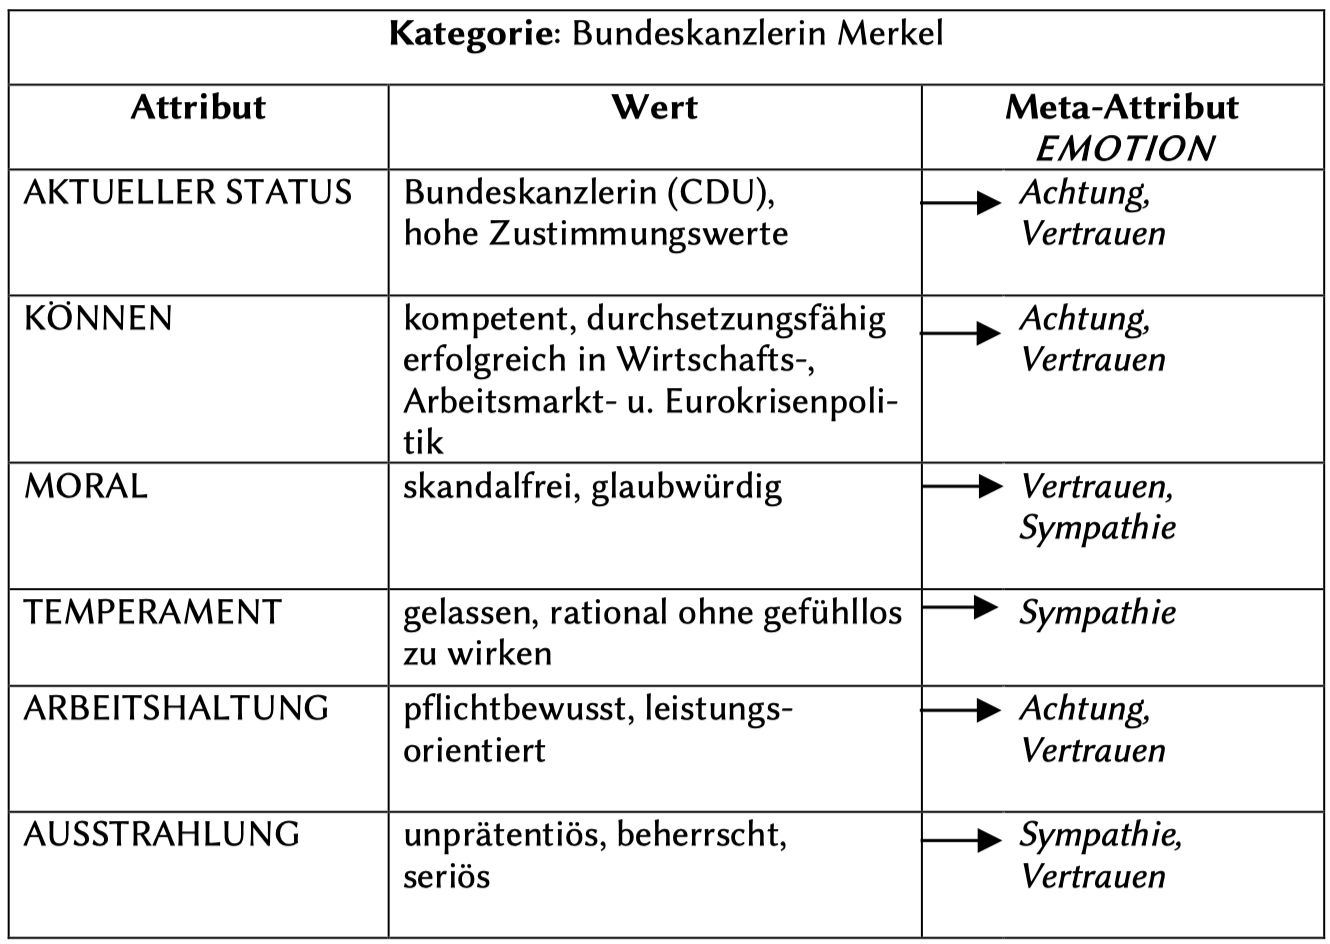
\includegraphics[width=\textwidth]{figures/media/image5.png}
  \caption{\label{fig:merkel-frame}Merkel-Ausgangs-Frame (Übersicht 5 aus \citealt[312]{kleinFrameUndFraming2018}). Legende: Pfeil: Kausalrelation (Ursache{\slash}Grund → Wirkung{\slash}Folge)}
\end{figure}

Das Ziel bestehe nun für die CDU darin,

\begin{quote}
die in den Ausgangsframes erfassten Vorstellungen im Sinne des Wahlzieles und der Hauptausrichtung der Kampagne zu modifizieren bzw. zu optimieren und als verbessertes Bild der CDU-Politik und der Kanzlerin in den Köpfen möglichst vieler Wahlberechtigter zu verankern. \autocite[314]{kleinFrameUndFraming2018}
\end{quote}

Dazu können zum einen die bestehenden Attribut-Wert-Konfigurationen gestärkt oder modifiziert werden, zum anderen können neue Attribut-Wert-Paare etabliert werden. Die beim Framing eingesetzten kommunikativen Mittel reichen dabei von einzelnen Formulierungen in Broschüren und Wahlreden bis hin zu Erzählungen aus dem Privatleben im Fernsehen sowie visuellem Framing auf Plakaten und im Fernsehen. Eine Kombination verschiedener Mittel wurde etwa eingesetzt, um \textsc{Wählernähe} als neues Attribut im Frame zu etablieren:

\begin{quote}
Merkels weithin hoch geschätzte Eigenschaft, unprätentiös zu sein, erleichterte Framing in Richtung ‚Normalisierung` der Bundeskanzlerin. Das geschah primär in Texten, aber auch in Bildern. Auf Merkels eigens für die Wahlkampagne eingerichteter sog. ‚Homepage` und in der damit text- und bild-identischen, massenhaft verteilten Merkel-Broschüre wird einerseits die entscheidungsstarke, durchsetzungsfähige Politikerin nicht verleugnet („ich will\ldots``; „ich entscheide...``), andererseits ist sie, wenn es um Privates geht, eine ‚wie du und ich`: „Ich koche sehr gern, am liebsten Rouladen und Kartoffelsuppe.`` Ihr Ehemann, ein „Konditorsohn`` beschwert sich, „auf dem Kuchen sind immer zu wenig Streusel.`` \autocite[315-316]{kleinFrameUndFraming2018}
\end{quote}

Ob es tatsächlich so simpel gelingen kann, neue bzw. modifizierte Frames in den Köpfen der Wähler*innen zu verankern, bleibt aber letztlich offen.\footnote{Klein verweist allerdings auf den Wahlerfolg der CDU als Indikator: „Zwar pflegen Wahlsiege viele Mütter und Väter zu haben, doch wäre es bei einem so klaren und hohen Wahlsieg wie dem der Union 2013 wenig rational anzunehmen, dass alles mögliche Andere für den Erfolg der Kampagne verantwortlich war, nur nicht das strategische Framing.`` \autocite*[327]{kleinFrameUndFraming2018}.}

Einen im Vergleich deutlich stärker deskriptiv ausgerichteten Framing-Begriff präsentieren Ziem et al. \autocite*{ziemMedienFramesAlsSemantische2018}. Zwar stimmen sie Klein grundsätzlich darin zu, dass „während Frames Wissensstrukturen repräsentieren und modellieren, {[}\ldots{]} sich der Begriff des Framing insbesondere auf den Prozess der Entstehung und Verfestigung dieser Strukturen {[}richtet{]}`` \autocite[159]{ziemMedienFramesAlsSemantische2018}. Sie differenzieren jedoch zwischen einem strategisch-intentionalen Framing im Sinne des „Begriffe besetzen`` \autocite{liedtkeBegriffeBesetzenStrategien1991}, wie es in den hier bisher betrachteten Framing-Konzepten angedacht ist, und einem Framing, das „emergent{[}es{]} Ergebnis des Sprachgebrauchs`` \autocite[159]{ziemMedienFramesAlsSemantische2018} und insofern ein Fall von „Begriffswandel`` \autocite{kellerSprachwandelUnsichtbarenHand2003} ist. Ähnlich wie Klein konzeptualisieren sie Framing als die variierende Instantiierung von Frame-Slots und -Fillern und nutzen für dessen analytische Erfassung und Beschreibung \emph{FrameNet}. Sie können so zeigen, dass im Kontext der Snowden-Affäre in der New York Times der \FN{Gathering\_up}-Frame mit anderen FE realisiert wird als in einem aus dem Open American National Corpus bezogenen Vergleichskorpus und etwa die Slots \textsc{Agens} und \textsc{Individuen}, d.\,h. die sammelnden Akteure und die gesammelten Objekte, deutlich häufiger realisiert werden, während FE wie \textsc{Zweck}, \textsc{Quelle} oder \textsc{Zeit} seltener instantiiert werden als im Vergleichskorpus.

Klein und Ziem verbinden die Frame- und die Framing-Theorie auf durchaus ähnliche Weise miteinander, geben jedoch keine bündige Definition für ihren Framing-Begriff. Für diese Arbeit sei daher als Arbeitsdefinition festgehalten, dass Framing die potentiell strategische Instantiierung eines Frames mit bestimmten Slots und Fillern meint. Instantiiert werden natürlich zunächst Token-Frames; durch Abstraktion kann aber auch auf Type-Frames geschlossen werden, die dann für einzelne Diskursbereiche ein bestimmtes Framing ausweisen. Hinsichtlich der Praxisorientierung des Framing-Begriffs folgt die Arbeitsdefinition Ziem et al. und fügt sich in den deskriptiven Gesamtansatz der vorliegenden Arbeit ein. Framing ist so zwar durchaus an sprachliches Handeln gebunden, kann aber zugleich (auch) als emergentes, unintentionales Phänomen verstanden werden. Diese Definition weist weitgehende Übereinstimmungen mit Busses Ausführungen zur Perspektivierbarkeit von Frames (\chapref{perspektivierung-kontext-und-frame-wandel}) auf, die er als „Aktivierung bestimmter Sub-Sets von Slots / Attributen aus der Gesamt-Menge von Slots / Attributen eines \emph{type}-Frames`` oder durch die „Füllung der Slots mit spezifischen (Sets von) Werten`` definiert \autocite[622]{busseFrameSemantikKompendium2012}. Wengelers Einwand, das Framing-Konzept eröffne der Linguistik kaum neue Analysemöglichkeiten, sondern habe nicht zuletzt „aufgrund seines modernen Touchs`` \autocite*[27]{wengelerWarnungVorFraming2022} Einzug in Frame-semantische Arbeiten erhalten, ist also nicht völlig von der Hand zu weisen. Meines Erachtens sind jedoch die Anschließbarkeit an die Kommunikations- und Medienwissenschaft inklusive der Unterlegung ihrer Framing-Theorie mit einem ausgearbeiteten Wissensmodell inklusive der präzisen Berücksichtigung sprachlicher Zeichen \autocite[176]{ziemMedienFramesAlsSemantische2018}, die gute Kommunizierbarkeit des Begriffs und letztlich auch die terminologische Eleganz („Frame ist Struktur. Framing ist Handeln.``, \citealt[289]{kleinFrameUndFraming2018}) gute Gründe, den Begriff auch in der Linguistik zu nutzen.

\section[Semantik, Pragmatik und das \emph{corpus-driven} Paradigma]{Distributionelle Semantik, Korpuspragmatik und das \emph{corpus-driven} Paradigma}\label{distributionelle-semantik-korpuspragmatik-und-das-corpus-driven-paradigma}
\subsection{Distributionelle Semantik}\label{distributionelle-semantik}

In den bisherigen Kapiteln wurde die Grundlage dafür gelegt, in Diskursen konstituierte und verhandelte Bedeutung mithilfe eines ausdifferenzierten linguistischen Modells beschreiben zu können. Auch wenn diesen Modellen zumeist die Annahme kognitiver, individueller Wissensbestände zugrundeliegt, wird zu ihrer Ermittlung in Frame-semantischen Analysen auf linguistische Methodik und Diskurskorpora zurückgegriffen (siehe \chapref{frames-und-kognition}). Da dabei auch quantitativ-korpuslinguistische Ansätze wie Keyword- oder Kollokations-Analysen auf fruchtbare Weise herangezogen werden \autocites[siehe u.\,a.][]{czuloEinflussExtremistischerGewaltereignisse2020, ziemMedienFramesAlsSemantische2018, ziem3WortschatzII2017, storjohannPrasenzUndAbsenz2013}, liegt es nicht fern, über eine vertiefte Integration Frame-semantischer Ansätze mit korpuslinguistischen Zugängen zur Semantik nachzudenken. Für letztere ist insbesondere das Paradigma der distributionellen Semantik ein wichtiger Rahmen. Seine Grundlagen wurden bereits in den 1950er Jahren gelegt, in denen die Distribution von Wörtern als höchst relevant für ihre semantische Beschreibung erkannt worden ist. Es ist dabei zum einen die Tradition des amerikanischen Strukturalismus, zum anderen die des britischen Kontextualismus, die die Entstehung distributionell-semantischer Ansätze prägen. Von amerikanisch-strukturalistischer Seite stellt Zellig Harris den Zusammenhang zwischen Bedeutung und Distribution heraus: „difference of meaning correlates with difference of distribution`` \autocite*[156]{harrisDistributionalStructure1954}. Diese Erkenntnis ist, so Lenci, der Ausgangspunkt für die ‚Distributionelle Hypothese`, die er folgendermaßen zusammenfasst: „Lexemes with similar linguistic contexts have similar meanings.`` \autocite[152]{lenciDistributionalModelsWord2018}. Etwas weiter gefasst formuliert Sahlgren:

\begin{quote}
The main point of this hypothesis is that there is a correlation between distributional similarity and meaning similarity, which allows us to utilize the former in order to estimate the latter. \autocite[33]{sahlgrenDistributionalHypothesis2008}
\end{quote}

Auch die Arbeiten John Rupert Firths, dem Begründer des britischen Kontextualismus, spielen in distributionell-semantischen Ansätzen eine wichtige Rolle. Er hat insbesondere die Bedeutung des Kotextes für die Semantik erkannt und in der berühmten Formel „You shall know a word by the company it keeps`` \autocite[11]{firthSynopsisLinguisticTheory1957} zusammengefasst. Auf Firth geht dabei auch das für die Korpuslinguistik zentrale Konzept der Kollokation zurück und er konstatiert, dass \emph{collocational meaning} eine von mehreren Bedeutungsdimensionen ist:

\begin{quote}
The following sentences show that part of the meaning of the word \emph{ass} in modern colloquial English can be by collocation:

(i) An ass like Bagson might easily do that.

(ii) He is an ass.

(iii) You silly ass!

(iv) Don't be an ass!

One of the meanings of \emph{ass} is its habitual collocation with an immediately preceding \emph{you silly}, and with other phrases of address or of personal reference. Even if you said „An ass has been frightfully mauled at the Zoo``, a possible retort would be, „What on earth was he doing?{}`` \autocite[194-195]{firthPapersLinguistics193419511957}
\end{quote}

In kontextualistischer Perspektive sind sprachliche Äußerungen dabei immer funktional zu denken und in rekurrente situative sowie diese umfassende kulturelle Kontexte eingebettet:

\begin{quote}
That is what language really means to us -- a way of doing things, a way of getting things done, a way of behaving and getting others to behave, a way of life. {[}\ldots{]} We can only arrive at some understanding of \emph{how} it works, if we establish with certainty that the facts of speech we are studying can be observed or regarded in actual patterns of behaviour. We must take our facts from speech sequences, verbally complete in themselves and operating in contexts of situation which are typical, recurrent, and repeatedly observable. Such contexts of situation should themselves be placed in categories of some sort, sociological and linguistic, within the wider context of culture. \autocite[35]{firthSynopsisLinguisticTheory1957}
\end{quote}

Diese kontextuelle Bedeutungsdimension unterscheidet er jedoch von der kotextuellen, über Kollokationen aufspürbaren\footnote{So konstatiert er: „It must be pointed out that meaning of collocation is not at all the same thing as contextual meaning, which is the functional relation of the sentence to the processes of a context of situation in the context of culture`` \autocite[195]{firthPapersLinguistics193419511957}.} und möchte letztere auch nicht mit konzeptueller Bedeutung verwechselt wissen:

\begin{quote}
Meaning by collocation is an abstraction at the syntagmatic level and is not directly concerned with the conceptual or idea approach to the meaning of words. \autocite[196]{firthPapersLinguistics193419511957}
\end{quote}

Distributionell-semantische Modelle lassen sich gemäß der von ihnen gemessenen distributionellen Achse in zwei Gruppen unterteilen: syntagmatische und paradigmatische Modelle \autocite[40]{sahlgrenDistributionalHypothesis2008}. Syntagmatische Modelle bilden dabei das gemeinsame Vorkommen von Wörtern ab, also z.\,B. dass das Wort \emph{festgenommen} mit Wörtern wie \emph{wurde}, \emph{Polizei}, \emph{Verdächtigen}, \emph{Personen} oder \emph{sieben} vorkommt (siehe \tabref{tab:collocations_neighbors}). Sie sind in Form der Kollokationsanalyse fester Bestandteil des (korpus\mbox{-})linguistischen Methodeninventars (siehe zur Methode der Kollokationsanalyse ausführlicher \chapref{kollokationen-als-syntagmatische-distributionelle-muster}). Paradigmatische Modelle hingegen fragen nicht nach den Nachbarn eines Wortes in Texten, sondern danach, welche Wörter ähnliche Nachbarn haben. Dazu werden Wörter i.d.R. in Vektoren, also Listen von Zahlen, überführt. Sie können dann in einem gemeinsamen vektorgeometrischen Raum abgebildet werden, wobei ihre Position in diesem Raum auf ihren Kotexten beruht und Wörter mit ähnlichen Kotexten nah beieinander positioniert sind. Die paradigmatische Ähnlichkeit bzw. Nähe im Vektorraum entspricht dabei diskurs- bzw. korpusspezifischer funktionaler Äquivalenz \autocite[587]{bubenhoferSemantischeAquivalenzGeburtserzahlungen2020}. Die nächsten paradigmatischen Nachbarn\footnote{Sinclair \autocite*[142]{sinclairTrustTextLanguage2004} nutzt auch für \emph{paradigmatische} Nachbarschaft in diesem Sinne den Begriff der Kollokation; üblicherweise -- und so auch in dieser Arbeit -- ist er aber der syntagmatischen Nachbarschaft vorbehalten.} zu \emph{festgenommen} sind in einem solchen Vektorraum Wörter wie \emph{inhaftiert}, \emph{beschuldigt}, \emph{getötet} oder \emph{geschnappt} (siehe \tabref{tab:collocations_neighbors}). Enorm an Popularität gewonnen haben paradigmatische distributionelle Modelle mit der Entwicklung moderner, ressourcensparsamer und auf neuronalen Netzen beruhender Algorithmen wie denen des \emph{Word2Vec}-Frameworks \autocite{mikolovEfficientEstimationWord2013}, mit denen sich solche Wortvektoren (Word Embeddings) berechnen lassen (siehe dazu ausführlich \chapref{word-embeddings-als-paradigmatische-distributionelle-muster}).

Allen distributionell-semantischen Modellen ist gemein, dass sie keine ‚unmittelbare`, referentielle Auskunft zur Bedeutung eines Wortes geben, sondern nur differentielle Informationen: Wir erfahren, wie Wörter in einem Korpus verteilt sind und inwiefern sich diese Verteilung von der anderer Wörter unterscheidet, können aber die Bedeutung von z.\,B. \emph{festgenommen} nicht unmittelbar ablesen. Sahlgren stellt heraus, dass sich daran der strukturalistische Charakter der distributionellen Semantik zeigt und ihr Bedeutungsbegriff dem Saussureschen Begriff des \emph{valeur} entspricht:
\largerpage[-2]
\begin{quote}
Similarly in la langue, signs are identified by their functional differences. Saussure used the term \emph{valeur} to describe the function of a sign. This is arguably the most important concept in structuralist theory, since it is a sign's valeur that defines its role within the language system. Valeurs are defined purely differentially, so that a sign has a valeur only by virtue of being different from the other signs. Such a differential view on the functional distinctiveness of linguistic elements highlights the importance of the system as a whole, since differences (i.e. valeurs) cannot exist in isolation from the system itself. A single isolated sign cannot enter into difference relations, since there are no other signs to differ from. In this view, the system itself becomes an interplay of functional differences \autocite[38]{sahlgrenDistributionalHypothesis2008}
\end{quote}

Dies macht Word Embeddings gerade für kulturbezogene Forschung zu einer hervorragenden Methode, denn die „fundamental insight that meaning is not immanent within words and phrases but rather coheres within a broader cultural system is inherent in any word embedding analysis'' \autocite[914]{kozlowskiGeometryCultureAnalyzing2019}. Ein weiteres Charakteristikum distributioneller Bedeutungsmodelle ist, dass sie durch und durch sprachgebrauchsbasiert, induktiv und korpusspezifisch sind. Sie grenzen sich somit von jeglichem Versuch einer introspektiven Sprachbeschreibung ab:

\begin{quote}
By grounding the representations in actual usage data, distributional approaches only represent what is \emph{really there} in the current universe of discourse. When the data changes, the distributional model changes accordingly; if we use an entirely different set of data, we will end up with an entirely different distributional model. Distributional approaches acquire meanings by \emph{virtue} of being based entirely on noisy, vague, ambiguous and possibly incomplete language data. \autocite[50]{sahlgrenDistributionalHypothesis2008}
\end{quote}

Die zentrale Stellung des Korpus in der distributionellen Semantik und die funktionale Perspektive auf Sprachzeichen korrespondiert eng mit theoretischen Überlegungen aus dem Bereich der Korpuspragmatik, die im folgenden Kapitel dargestellt werden sollen.

\subsection{Korpuspragmatik}\label{korpuspragmatik}

Den Begriff der Korpuspragmatik definieren Felder et al. \autocite*{felderKorpuspragmatikParadigmaZwischen2012} in der Einleitung zum von ihnen herausgegebenen gleichnamigen Sammelband als

\begin{quote}
linguistischen Untersuchungsansatz, der in digital aufbereiteten Korpora das Wechselverhältnis zwischen sprachlichen Mitteln einerseits und Kontextfaktoren andererseits erforscht und dabei eine Typik von Form-Funktions-Korrelationen herauszuarbeiten beabsichtigt. Solche Kontextfaktoren betreffen potenziell die Dimensionen \emph{Handlung}, \emph{Gesellschaft} und \emph{Kognition}. Die Analyse bedient sich insbesondere einer Kombination qualitativer und quantitativer Verfahren. \autocite[4-5]{felderKorpuspragmatikParadigmaZwischen2012}
\end{quote}

Ausgegrenzt aus dem Zielgebiet korpuspragmatischer Studien werden somit solche korpuslinguistischen Ansätze, die ein „sprachstrukturimmanentes Interesse haben``, also etwa zu lexikologischen oder grammatischen Fragestellungen arbeiten \autocite[4]{felderKorpuspragmatikParadigmaZwischen2012}. Sprachliche Bezugsgröße ist für sie der Diskurs im Sinne des Sprachgebrauchs \autocite{fasoldSociolinguisticsLanguage1990}, den sie mit van Dijk \autocite*{vandijkDiscourseContextSociocognitive2008} als multimodal begreifen und dessen „Handlungscharakter`` sie hervorheben \autocite[5]{felderKorpuspragmatikParadigmaZwischen2012}. Eine weitere Grundannahme der Korpuspragmatik ist im Anschluss an Feilke \autocite*{feilkeSpracheAlsSoziale1996} und Tomasello \autocite*{tomaselloKonstruktionsgrammatikUndFrueher2006} „das Theorem {[}\ldots{]}, dass die Regelhaftigkeit von Sprache sich aus der Regelhaftigkeit von Verwendungssituationen ableitet`` \autocite[5]{felderKorpuspragmatikParadigmaZwischen2012}. Hierauf stützen sie auch die zentrale Rolle von Kontexten als „verstehensrelevante Deutungsrahmen`` \autocite[6]{felderKorpuspragmatikParadigmaZwischen2012} und heben die epistemische Rolle sprachlicher Zeichen und Muster hervor:

\begin{quote}
Bedenkt man in diesem Zusammenhang, dass ein großer Teil unseres individuellen Wissens auf der Rezeption von Sprachzeichen, wie sie in sprachlichen Äußerungen mündlicher und schriftlicher Art verbreitet werden, basiert, so ist evident, dass die auf diese Weise gewonnenen Wissensbestände und Erfahrungen in kommunikativen Formulierungsroutinen reproduziert und dadurch teilweise zu „kollektiven`` Wissensbeständen bzw. Erfahrungsmustern verdichtet werden. \autocite[6]{felderKorpuspragmatikParadigmaZwischen2012}
\end{quote}

Dieser epistemologische Fokus sowie die Handlungs- und Gesellschaftsorientierung der Korpuspragmatik machen auch die Forschungsgegenstände einer Diskurslinguistik nach Foucault \autocite{warnkeDiskurslinguistikNachFoucault2007a} zum Thema der Korpuspragmatik. Zu den wissensorientierten diskurslinguistischen Arbeiten konstatieren sie jedoch:

\begin{quote}
In diesem Bereich ist das korpuslinguistische Vorgehen nicht sonderlich weit verbreitet. Das erklärt sich leicht dadurch, dass Wissensbestände nur interpretativ aus Texten plausibel gemacht werden können, ein qualitativer Zugang also unumgänglich erscheint. Allerdings haben sich hier korpuslinguistische Methoden zur Vorstrukturierung und Identifizierung zentraler Diskursmuster bewährt, in denen Wissenskonfigurationen ausgedrückt sind. \autocite[14]{felderKorpuspragmatikParadigmaZwischen2012}
\end{quote}

Meines Erachtens wirft diese Konzeption zur Rolle korpuslinguistischer Verfahren jedoch mehrere Fragen auf. Erstens sind korpuslinguistische Verfahren m.\,E. nicht mit einem quantitativen Zugang gleichzusetzen. So wird -- gerade in den englischsprachigen \emph{corpus-assisted discourse studies} (CADS) -- die Bedeutung der Lektüre von Konkordanzen oder auch längerer Textpassagen immer wieder hervorgehoben \autocite[siehe etwa][7]{gillingsTakingRoadLess2024}. Zweitens wird hier m.\,E. eine -- im Bereich der diskurslinguistischen Wissensanalyse allerdings in der Tat weit verbreitete -- Fehlannahme reproduziert, die das Verhältnis von quantitativer Korpuslinguistik, Interpretation und Wissensbeständen als Analyseobjekt betrifft. So ist es zwar in der Tat so, dass „Wissensbestände nur interpretativ aus Texten plausibel gemacht werden können`` -- dies bedeutet aber nicht, dass dies auf der Basis eingehender, qualitativer Textlektüren erfolgen muss. Auch quantitative, aus Texten gewonnene Daten müssen interpretiert werden und auch aus ihnen können Wissensbestände erschlossen werden (siehe dazu auch \chapref{begriffsklaerungen-quantitativ-und-qualitativ-corpus-driven-und-corpus-based-sowie-die-rolle-von-hermeneutik}). Letztlich ist auch zu fragen, warum quantitative Verfahren, wenn sie doch eine „Vorstrukturierung und Identifizierung zentraler Diskursmuster {[}\ldots{]}, in denen Wissenskonfigurationen ausgedrückt sind``, leisten können, nicht geradezu dafür prädestiniert sein sollten, um in epistemologisch-diskurslinguistischen Analysen eingesetzt zu werden. So ist doch zu bezweifeln, dass qualitative Methoden mehr leisten können, als Texte zu strukturieren, um in ihnen relevante Diskursmuster zu identifizieren. Einen irgendwie gearteten ‚direkten` Zugang zum diskursiv verhandelten Wissen bieten auch sie nicht.

Während bei Felder et al. \autocite*[4-5]{felderKorpuspragmatikParadigmaZwischen2012} die bevorzugte „Kombination qualitativer und quantitativer Verfahren`` gar definitorischen Rang für das korpuspragmatische Paradigma erhält, hat sich in den Arbeiten von Noah Bubenhofer und Joachim Scharloth ein deutlich stärker quantitativ akzentuierter Begriff der Korpuspragmatik herausgebildet. Sie definieren einen korpuspragmatischen Zugang wie folgt:

\begin{quote}
Die Korpuspragmatik deutet signifikant häufig auftretende sprachliche Muster in Korpora als Ergebnis rekurrenter Sprachhandlungen der Autorinnen und Autoren der im Korpus enthaltenen Texte bzw. der sie autorisierenden Institutionen und Gruppen. Sie geht davon aus, dass sich pragmatische Informationen „im pragmatischen Mehrwert oder Gebrauchswert von Einheiten aller sprachlicher Strukturbereiche`` (Feilke 2000: 78) zeichenhaft manifestiert. Damit werden pragmatische Spuren an der sprachlichen Oberfläche als Muster, in die sich ein Gebrauchswert eingeschrieben hat, sichtbar (vgl. zu dieser Rehabilitierung der Textoberfläche auch den Sammelband von Feilke{\slash}Linke 2009). Diese „Sprachgebrauchsmuster`` (Bubenhofer 2009) werden damit als Ergebnis von sprachlich-sozialem Handeln gelesen und gedeutet. \autocite[148-149]{bubenhoferKorpuslinguistischeDiskursanalyseNutzen2013}
\end{quote}

Auch Bubenhofer \& Scharloth heben also mit Feilke den Nexus zwischen wiederholtem (sprachlichen) Handeln und sprachlichen Mustern auf der Textoberfläche hervor. Mit dem statistischen Konzept der signifikanten Häufigkeit ist bei ihnen allerdings ein quantitativer, d.\,h. auf Frequenzen operierender, Zugang vorausgesetzt. Dieser erlaubt zugleich ein induktives, \emph{corpus-driven} \autocite{tognini-bonelliCorpusLinguisticsWork2001} Vorgehen, für das die Autoren sich aussprechen, da es Befunde ermöglicht, „die entweder quer zu den vorher existierenden Erwartungen stehen und die Grundlage für neue Hypothesen sind, oder im besten Fall sogar solche Evidenzen, die die Bildung neuer interpretativer linguistischer Analysekategorien nahelegen`` \autocite[149]{bubenhoferKorpuslinguistischeDiskursanalyseNutzen2013}. Diese Potenziale sind für Frame-semantische Diskursanalysen äußerst vielversprechend, da sie helfen können, FE eines Frames aufzudecken. So warnen auch Scholz \& Ziem in Hinblick auf rein deduktive Analysen, es könne

\begin{quote}
sich ein gravierendes methodologisches Problem ergeben, wenn die Annotationen ausschließlich auf den vorgegebenen Kategorien -- d.\,h. den Prädiktoren in Matrixframes und Frame-Elementen in FrameNet-Frames -- beruhen: Das vordefinierte Set an Leerstellen bzw. Frame-Elementen determiniert den Such- und Annotationsbereich derart, dass außerhalb dessen keine Annotationen vorgenommen werden können. Zugespitzt formuliert: Es lässt sich nur das finden, was mittels der vorgegebenen Annotationskategorien auch gesucht wird. Dieses Dilemma lässt sich nur mittels einer induktiven Untersuchungsheuristik vollständig beheben. \autocite[306]{scholzVokabularImDiskurshistorischen2015}
\end{quote}

Ein weiterer gewichtiger Vorteil liegt m.\,E. darin, dass den Ergebnissen von \emph{corpus-driven} Methoden „sämtliche Zeichenkonfigurationen {[}\ldots{]}, die sich bei der Anwendung vorher festgelegter Algorithmen ergeben`` \autocite[149]{bubenhoferKorpuslinguistischeDiskursanalyseNutzen2013}, zugrundeliegen. Wenn sie also zur Bildung linguistischer Kategorien im Sinne von FE geeignet sind und auf sprachlichen Zeichenkonfigurationen beruhen, könnten sie auch helfen, sich dem Ziel einer linguistischen Epistemologie, alle sprachlichen Mittel zu identifizieren, die mit einem Frame bzw. den einzelnen FE verbunden sind, zumindest deutlich näher zu kommen, als es in qualitativen Ansätzen je geleistert werden könnte. Die folgenden beiden Kapitel werden Bubenhofers \autocite*{bubenhoferSprachgebrauchsmusterKorpuslinguistikAls2009} Begriff des Sprachgebrauchmusters, der in dieser Variante der Korpuspragmatik zentral ist, sowie den von den Autoren verfolgten \emph{corpus-driven} Ansatz darstellen.

\subsection{Sprachgebrauchsmuster}\label{sprachgebrauchsmuster}

In der germanistischen korpusbasiert arbeitenden Diskurslinguistik ist das bereits angesprochene \emph{corpus-driven} Paradigma, das im folgenden Kapitel noch ausführlicher vorgestellt werden wird, insbesondere mit den Arbeiten Noah Bubenhofers und Joachim Scharloths verbunden \autocites[siehe zu \emph{corpus-driven} Zugängen in der Phraseologie und Grammatik etwa][]{belicaKorpusanalytischeZugangeSprachlichem2008, brunnerCorpusDrivenStudyMultiWord2007, kupietzGebrauchsbasierteGrammatikStatistische2009}. Die grundlegende Operationalisierung korpuslinguistischer Zugänge für die Diskursanalyse leistet dabei Bubenhofer \autocite*{bubenhoferSprachgebrauchsmusterKorpuslinguistikAls2009}, der in einer \emph{corpus-driven} verfahrenden Analyse Diskurse anhand von Sprachgebrauchsmustern, d.\,h. musterhaftem Sprachgebrauch auf der sprachlichen Oberfläche, rekonstruiert. Eine Besonderheit stellt auch der Verzicht auf bzw. sogar die explizite Ablehnung einer thematischen Definition von Diskursen und Diskurskorpora, wie sie im einschlägigen Aufsatz von Busse und Teubert \autocite*{busseIstDiskursSprachwissenschaftliches1994} für die germanistische Diskurslinguistik gefordert und geprägt wird, dar. Als Gründe führt Bubenhofer die Unvoreingenommenheit einer solchen Analyse an, die die Replizierung bereits angenommener Diskurse und Diskursstrukturen vermeidet:

\begin{quote}
Die Frage nach der Repräsentativität des Korpus zeigt, dass Busse/ Teubert (1994, 14f.) diese nach inhaltlichen Kriterien festlegen, was zu einer manuellen Auswahl von „relevanten`` Texten führt. Diese Beschränkung ist nicht nur unnötig, sondern auch kritisch, wenn das Ziel einer Diskursanalyse darin besteht, auch verborgene und unauffällige Strukturen aufzuzeigen. Relevanzempfinden ist ein Ergebnis diskursiver Formationen. Dieses als Kriterium zu wählen, bedeutet, die offensichtlichen Strukturen des Diskurses zu replizieren. \autocite[36]{bubenhoferSprachgebrauchsmusterKorpuslinguistikAls2009}
\end{quote}

Sprachgebrauchsmuster definiert Bubenhofer als „textoberflächlich{[}e{]} Indikator{[}en{]} für soziales Handeln`` \autocite*[55]{bubenhoferSprachgebrauchsmusterKorpuslinguistikAls2009}, und beschreibt ihre diskursive Funktion mit Linke als „minimale Kristallisationskerne`` \autocite*[40]{linkeBegriffsgeschichteDiskursgeschichteSprachgebrauchsgeschichte2003} von Diskursen. In der \emph{Parole} zu findende Sprachgebrauchsmuster ermöglichen somit einen „Zugriff auf epistemisches Wissen {[}\ldots{]} und damit auf Diskurse`` \autocite[53]{bubenhoferSprachgebrauchsmusterKorpuslinguistikAls2009}:

\begin{quote}
Sprachgebrauchsmuster sind Ausdruck sozialen Handelns und bestimmte Sprachgebrauchsmuster können deshalb als Indikatoren für bestimmtes soziales Handeln gelesen werden. \autocite[53]{bubenhoferSprachgebrauchsmusterKorpuslinguistikAls2009}
\end{quote}

Mit dem Ziel, idiomatische Prägungen im Sinne von Feilke \autocite*{feilkeSprachlicherCommonSense1993} abzubilden, betrachtet Bubenhofer ausschließlich Mehrworteinheiten als Sprachgebrauchsmuster. Operationalisiert werden diese für den korpuslinguistischen Zugriff als signifikante N-Gramme, also in einzelnen Teilkorpora überzufällig häufig unmittelbar aufeinander folgende Token. Die signifikanten Mehrworteinheiten als solche stellen allerdings noch keine Sprachgebrauchsmuster dar, sondern erhalten diesen Status erst nach ergänzenden kategorisierenden und interpretierenden \emph{corpus-based} Analysen.

Ausgehend von den Sprachgebrauchsmustern gelingt es Bubenhofer so, ein thematisch heterogenes Zeitungskorpus in unterschiedliche Teile -- in seinem Verständnis ‚Diskurse` -- zu gliedern und zu beschreiben. Für den Zeitraum 2003--2005 und das Auslandsressort der NZZ (\textsc{Neue Zürcher Zeitung}) fördert seine Analyse z.\,B. die Mehrworteinheiten \emph{Kampf gegen Terrorismus}, \emph{im Irak die}, \emph{Präsident Bush in} und \emph{Usama bin Ladin} zu Tage, die in diesem Teilkorpus signifikant häufiger als im restlichen Korpus auftreten und sich unschwer auf den Irakkrieg zurückführen lassen \autocite[209-210]{bubenhoferSprachgebrauchsmusterKorpuslinguistikAls2009}. Solche Gruppen von Sprachgebrauchsmustern können sodann als „Hinweise auf Diskurse`` \autocite[295]{bubenhoferSprachgebrauchsmusterKorpuslinguistikAls2009} aufgefasst werden, etwa zu Themen wie ‚Krieg und Gewalt` oder ‚Sorgen und Probleme` und sie übernehmen in diesen Diskursen je spezifische, mitunter auf subtile Art ausdifferenzierte Funktionen:

\begin{quote}
Bei der Analyse der Kontextualisierungsprofile von \emph{Kampf gegen X}, \emph{Kampf dem X} und \emph{Kampf mit X} haben sich deutliche Differenzen im Gebrauch gezeigt. Dabei handelt es sich nicht nur um semantische Präferenzen {[}\ldots{]}, sondern um pragmatisch unterschiedliche Funktionen. So wird der \emph{Kampf gegen den Terror} im Ausdruck \emph{Kampf dem Terror} zur Parole; der Ausdruck findet sich besonders häufig in argumentativen Kontexten und zeigt eine Distanzierung oder Kritik an. \autocite[303]{bubenhoferSprachgebrauchsmusterKorpuslinguistikAls2009}
\end{quote}

Dass Bubenhofers Diskursbegriff dabei letztlich auf einer formalen Ebene bleibt und sich gegen thematische Diskursdefinitionen dezidiert abgrenzt, führt dazu, dass die beschriebenen Diskurse mitunter eher vage umrissen sind und einander überlappen. So resümiert er:

\begin{quote}
Der induktive Zugang ist also nicht vorurteilslos, aber er definiert seine Grundannahmen anders als es z.\,B. semantisch-tiefenstrukturelle Analysen tun. Und dieser Zugang führt dann auch zu einem bunten Strauß an Sprachgebrauchsmustern, die einerseits eher Kristallisationspunkte des inhaltlich Sagbaren, andererseits der Sprechweisen, der diskursiven Praxis darstellen. Diese Heterogenität ist auf der Ebene der Analyse nicht immer einfach zu handhaben und es ist kaum möglich, daraus homogene Diskursbeschreibungen abzuleiten. \autocite[311]{bubenhoferSprachgebrauchsmusterKorpuslinguistikAls2009}
\end{quote}

Eine solche Einschränkung wäre für die Diskurslinguistik, die ja i.d.R. an der Untersuchung aktueller und gesellschaftlich relevanter thematischer Diskurse interessiert ist, durchaus hinderlich. Es ist m.\,E. jedoch zu prüfen, ob die von Bubenhofer vorgenommene Trennung zwischen thematischen und entlang von Sprachgebrauchsmustern definierten Diskursen wirklich notwendig ist. So sind Themen ja ebenfalls Bedeutungskomplexe -- und wenn Sprachgebrauchsmuster „kleinste semantische Einheiten`` \autocite[336]{bubenhoferSprachgebrauchsmusterKorpuslinguistikAls2009} sind, sollte es möglich sein, anhand von Sprachgebrauchsmustern auch klassische Themen zu rekonstruieren. Es erscheint aus umgekehrter Blickrichtung ja auch unplausibel, dass sich Themen nicht in musterhaftem Sprachgebrauch, allen voran dem rekurrenten Gebrauch eben thematisch einschlägiger Lexik, niederschlagen sollten. In der vorliegenden Arbeit gilt es also zu prüfen, ob in der sprachlichen Oberfläche und der Distribution von Wörtern sowie unter Einbezug neuerer methodischer Entwicklungen nicht doch ausreichend semantische Informationen vorliegen, um aus ihnen auch klassische Themen bzw. thematische Frames wie einen Extremismus-Frame rekonstruieren zu können. Der \emph{corpus-driven} Ansatz, der dabei zugrundegelegt wird, soll im folgenden Kapitel näher erläutert werden, wobei auch auf grundlegende Annahmen des britischen Kontextualismus sowie seiner korpuslinguistischen Weiterentwicklung durch Sinclair und Tognini-Bonelli eingegangen wird.

\subsection{\texorpdfstring{Der \emph{corpus-driven} Ansatz}{Der corpus-driven Ansatz}}\label{der-corpus-driven-ansatz}

Methodologischer Rahmen einer korpuslinguistischen und -- Bubenhofer und Scharloth folgend -- auch einer korpuspragmatischen Perspektive auf Sprache ist der \emph{corpus-driven}-Ansatz, wie er von Tognini-Bonelli \autocite*{tognini-bonelliCorpusLinguisticsWork2001} in Abgrenzung zum \emph{corpus-based} Ansatz vorgeschlagen wurde. Beide Vorgehensweisen werden im Folgenden vorgestellt, bevor sie in \chapref{begriffsklaerungen-quantitativ-und-qualitativ-corpus-driven-und-corpus-based-sowie-die-rolle-von-hermeneutik} auch von der Differenzierung qualitativ -- quantitativ unterschieden werden.

Das \emph{corpus-based}-Paradigma wird von Tognini-Bonelli als eine Methodologie gefasst, die Korpora hauptsächlich dafür verwendet, bereits existente Hypothesen zu elaborieren, zu prüfen oder zu belegen. Diese Herangehensweise

\begin{quote}
avails itself of the corpus mainly to expound, test or exemplify theories and descriptions that were formulated before large corpora became available to inform language study. \autocite[65]{tognini-bonelliCorpusLinguisticsWork2001}
\end{quote}

Das Korpus dient hier im Wesentlichen dazu, den Anteil, den Intuition und Sprachgefühl in introspektiv verfahrenden Analysen haben, durch einen empirischen Zugang zu ersetzen bzw. ergänzen. Theorien müssen nun operationalisiert und in einem entsprechend aufbereiteten Korpus untersucht werden:

\begin{quote}
Traditionally, linguistic theories are the result of reflection by a scholar after absorbing a great deal of experience of language and languages, and testing the implications and consequences with reference to the intuition of competent or native speakers. The precise nature of the language experience is impossible to ascertain because it figures only as part of the linguist's credentials, and not as part of the methodology of research. If a corpus was to be used to evaluate one of this class of theories, the theory would have to be put into an explicit form so that those aspects of corpus patterning that it covered could be distinguished from those where the theory did not cover, or was at variance with, the evidence. Such a relationship between theory and data is the classical one in linguistics. \autocite[65]{tognini-bonelliCorpusLinguisticsWork2001}
\end{quote}

Korpuslinguistik hat in diesem Ansatz also den klaren Status einer Methode, deren Verdienst es ist, linguistisches Arbeiten empirisch zu fundieren, was zur Widerlegung oder Präzisierung zahlreicher zuvor introspektiv gewonnener Annahmen über Sprache führt. Die Operationalisierung besteht dabei in der Regel in der Erstellung von Kategorien, die es in den Daten wiederzufinden gilt, sodass mithilfe empirischer Belege die Theorie bestätigt, widerlegt oder modifiziert werden kann, ohne dabei jedoch grundlegend neue theoretische Impulse zulassen zu können:

\begin{quote}
The corpus is considered useful because, on occasions, it indicates where minor corrections and adjustments can be made to the model adopted and, of course, it can also be valuable as a source of quantitative evidence. In this case, however, corpus evidence is brought in as an extra bonus rather than as a determining factor with respect to the analysis, which is still carried out according to pre-existing categories; although it is used to refine such categories, it is never really in a position to challenge them as there is no claim made that they arise directly from the data. \autocite[66]{tognini-bonelliCorpusLinguisticsWork2001}\footnote{Anzumerken ist hier, dass \emph{corpus-based}-Ansätze, wie sie heute i.d.R. praktiziert werden, durchaus geeignet sind, neue Kategorien zu entdecken. Funde in den Daten, die quer zu den bestehenden Analyseschemata liegen, stellen dann in einem iterativen Prozess einen Ausgangspunkt für die Bildung neuer Kategorien dar.}
\end{quote}

Das \emph{corpus-driven}-Paradigma setzt sich in grundlegender Weise von dieser deduktiven Herangehensweise ab. Das Korpus dient hier nicht als bloßer Datensatz, in dem Belege gefunden und Hypothesen überprüft werden können, sondern ist Grundlage für die aufzudeckenden Kategorien:

\begin{quote}
The corpus-driven approach {[}\ldots{]} aims to derive linguistic categories systematically from the recurrent patterns and the frequency distributions that emerge from language in context. \autocite[87]{tognini-bonelliCorpusLinguisticsWork2001}.
\end{quote}

Jegliche Erkenntnis wird hier also in einem engen Zusammenspiel mit den Korpusdaten bzw. aus ihnen heraus entwickelt -- „the theoretical statement can only be formulated in the presence of corpus evidence and is fully accountable to it`` \autocite[11]{tognini-bonelliCorpusLinguisticsWork2001}. Ausgangspunkt, Untersuchungsobjekt und -- in neu strukturierter, durchmusterter und informativ angereicherter Form -- letztlich auch Output einer \emph{corpus-driven} Analyse ist also die \emph{Parole}. Diese durch und durch empirische, sprachgebrauchsorientierte Ausrichtung teilt die Korpuslinguistik mit der linguistischen Diskursanalyse im Allgemeinen \autocite[27-29]{spitzmullerDiskurslinguistikEinfuhrungTheorien2011}.

Die Bedeutung der Umkehr der Erkenntnisrichtung von ‚von der Theorie zu den Daten` zu ‚von den Daten zur Theorie` geht jedoch darüber hinaus, dass neue, frequenzbasierte Methoden zur Analyse auch großer Korpora genutzt werden können. Sie eröffnen außerdem eine grundlegend neue Perspektive auf Sprache, in der sprachliche Ausdrücke immer als kontextuell geprägt gelesen werden. Trennungen wie die von Semantik und Pragmatik, von Ausdrucks- und Äußerungsbedeutung, von Ko- und Kontext werden damit zu höchstens graduellen und orientierenden Vereinfachungen; sprachliche Muster -- besonders deutlich ist dies an einzelnen Wörtern sichtbar -- sind nicht isoliert beschreibbar, sondern immer nur als Teil von Texten, situativen Kontexten und mithin Kultur:

\begin{quote}
The corpus-driven approach {[}\ldots{]} aims to derive linguistic categories systematically from the recurrent patterns and the frequency distributions that emerge from language in context. Taking this one step further, we could say that it goes along with a holistic approach to language in that the cumulative effect of repeated instances is taken to reflect the semiotic system; the text is seen as an integral part of its verbal context and, ultimately, no discontinuity is assumed between this and the wider context of situation, and the even wider context of culture. \autocite[87]{tognini-bonelliCorpusLinguisticsWork2001}\footnote{Sie scheint an dieser Stelle über Firth hinauszugehen, der \emph{collocational} und \emph{contextual meaning} noch dezidiert voneinander abgegrenzt hat (siehe \chapref{distributionelle-semantik}).}
\end{quote}

Die Bedeutung des sprachlich Musterhaften in Form dieser „repeated instances`` ist in diesem Ansatz, auf den auch Felder et al. \autocite*[3-4]{felderKorpuspragmatikParadigmaZwischen2012} bei ihrem Entwurf der Korpuspragmatik Bezug nehmen, zentral gestellt. Begründet wird dies von Tognini-Bonelli mit Verweis auf den britischen Kontextualismus, wo schon Firth ebendiese als „central evidence of what people do, how language functions and what language is about`` \autocite[89]{tognini-bonelliCorpusLinguisticsWork2001} erkannt hat. Doch was sind diese „repeated instances`` bzw. „repeated events``, die es aus dem „mush of general goings-on'' \autocite[187]{firthPapersLinguistics193419511957} herauszuarbeiten gilt? Dies fasst Tognini-Bonelli zunächst vergleichsweise simpel als ein „pattern of occurrence`` \autocite*[89]{tognini-bonelliCorpusLinguisticsWork2001}, das mindestens zwei Mal vorkommt. Um der bloßen Erfassung von „personal idiosyncrasy`` vorzubeugen, sollen die beiden Vorkommen im Korpus außerdem unabhängig voneinander, das heißt z.\,B. nicht im gleichen Text, vorkommen. Während die Möglichkeit der Erkennung von Mustern generell von der formalen Aufbereitung des Korpus abhängt, wobei einzelne Wörter oder Phrasen immer potentiell signifikant sind \autocite[89]{tognini-bonelliCorpusLinguisticsWork2001}, macht sie als die zwei zentralen Elemente musterhaften Sprachgebrauchs im Korpus die Firthschen Konzepte \emph{collocation} und \emph{colligation} aus. Kollokationen fasst sie dabei mit Clear \autocite*[277]{clearFirthPrinciplesComputational1993} als „recurrent co-occurrence of words'', die unmittelbar beobachtbar sind und vergleichsweise einfach mithilfe korpuslinguistischer Tools berechnet werden können. Den Begriff \emph{colligation} übernimmt sie direkt von Firth \autocite*[23]{firthSelectedPapersFirth1968}; er bezeichnet damit „the interrelations of syntactical categories`` in Form von Wort- und Satzarten. Für das \emph{corpus-driven}-Paradigma modifiziert Tognini-Bonelli diese Definition und rückt das Token als Einheit der \emph{Parole} zu Ungunsten abstrahierender \emph{Langue}-Kategorien in den Mittelpunkt:

\begin{quote}
In the light of corpus evidence, however, the concept of colligation is being extended to include the syntactic constraints, or indeed preferences, that a specific word, seen as a unique lexical item rather than as a member of its class, entertains within its environment. \autocite[89]{tognini-bonelliCorpusLinguisticsWork2001}
\end{quote}

Letztlich ist es die Zusammenführung von \emph{collocation} und \emph{colligation}, die für sie Muster ausmachen:

\begin{quote}
Collocational and colligational patterns will, together, form the basis of the formalisation of repeated events. Only a descriptive statement that identifies their interconnections will yield insights into meaning. The notion of `pattern' as the meeting point between lexis and grammar thus becomes central to corpus-driven linguistics. \autocite[90]{tognini-bonelliCorpusLinguisticsWork2001}
\end{quote}

Sie führt außerdem Hunston \& Francis an, die in ihrer \emph{Pattern Grammar} die „patterns of a word`` folgendermaßen definieren:

\begin{quote}
The patterns of a word can be defined as all the words and structures which are regularly associated with the word and which contribute to its meaning. A pattern can be identified if a combination of words occurs relatively frequently, if it is dependent on a particular word choice, and if there is a clear meaning associated with it. \autocite[37]{hunstonPatternGrammarCorpusDriven2000}
\end{quote}

Dadurch, dass systemlinguistische Vorannahmen hier zunächst zurückgestellt werden und stattdessen von Grunde auf nach den Kombinationsmöglichkeiten von Wörtern und ‚Strukturen` und den mit ihnen einhergehenden Bedeutungsveränderungen gefragt wird, ändert sich die „unit of currency for linguistic description`` \autocite[91]{tognini-bonelliCorpusLinguisticsWork2001}. Statt einzelne Lemmata bzw. Lexeme als Grundeinheit zu nehmen, zeigt Tognini-Bonelli an verschiedenen Beispielen, dass weder die oftmals angenommene semantische Einheit von Wortform und Lexem noch die konventionelle Trennung von Wörtern entlang von Leerzeichen durchweg haltbar bzw. semantisch sinnvoll ist. Semantische Differenzen im Flexionsparadigma eines Lexems führt sie u.\,a. am Beispiel der Wortformen \emph{facing} und \emph{faced} vor, die in unterschiedlichen Korpora jeweils unterschiedliche Gebrauchspräferenzen aufweisen:

\begin{quote}
So with \emph{facing} in the Birmingham corpus we find words such as \emph{forwards}, \emph{palms}, \emph{stood} {[}\ldots{]} which are very obviously related to position. We find also words that relate to the more abstract notion which has to do with confronting problematic areas: \emph{problems}, \emph{problem}, \emph{fear}, \emph{serious}, but as we can see they are relatively rare compared to the first group, so we could conclude that in a corpus of general English the physical meaning of \emph{facing}, indicating position and direction, is much more common than the abstract one. It is interesting to note that the same generalisation does not apply to the \emph{Economist \& WSJ} corpus where the collocates of \emph{facing} are consistently abstract. Considering now the form \emph{faced}, we do not find a parallel with the preference for the physical use either in the Birmingham or in the \emph{Economist \& WSJ} corpora {[}\ldots{]}. The two inflected forms have taken on different roles and this specialisation according to word form has also followed register boundaries between a more general purpose corpus and a more specialised corpus such as the \emph{Economist} and \emph{WSJ} corpus. \autocite[95]{tognini-bonelliCorpusLinguisticsWork2001}
\end{quote}

Dieser Befund weist zum einen auf den Wert von \emph{corpus-driven} Analysen hin, um solcher Unterschiede überhaupt gewahr zu werden. Insbesondere mit ihrer Hilfe ist es möglich, das aufzuspüren, was Feilke \& Linke (aus nicht primär korpuslinguistischer Perspektive) den „kommunikativen Mehrwert sprachlicher Performanz`` nennen. Dieser entzieht sich durch das „Faktum, dass häufig mögliche Ausdrucksvarianten im Sprachgebrauch eingeschränkt werden bzw. eine spezifische Variante präferiert wird, ohne dass eine semantische oder pragmatische Begründung auf der Hand läge`` \autocite[5-6]{feilkeOberflaecheUndPerformanz2009}, oftmals der Intuition. Der Befund ist zum anderen auch für die Frame-semantische Modellierung äußerst bedeutsam und deutet Probleme an, die eine lemmabasierte und nicht nach Register bzw. Kontext spezifizierte Zuordnung von LE zu Frames birgt (siehe auch \chapref{warum-frames}).

Der zweite erwähnte Punkt betrifft Bedeutungseinheiten, die sich über die klassischen Wortgrenzen hinaus erstrecken und für die Sinclair \autocite*{sinclairUnitsMeaning1996} den Begriff der \emph{extended units of meaning} geprägt hat. Grundlage für diese Annahme ist die Beobachtung, dass Wörter gemeinsam auftreten und dabei keine eigenständigen Bedeutungen bewahren. So definiert Tognini-Bonelli den hier einschlägigen Begriff der \emph{co-selection}, der auf Arbeiten Sinclairs zurückgeht als

\begin{quote}
the habitual selection of two or more items together. The tendency of the words to co-occur is so strong that they cannot retain independent meanings. The most obvious types of co-selection, and the ones that are traditionally acknowledged, are idioms and compounds, where two or more words with independent meaning combine to form a new meaning (e.g. \emph{vacuum cleaner}; \emph{it's raining cats and dogs}). \autocite[101]{tognini-bonelliCorpusLinguisticsWork2001}
\end{quote}

\emph{Co-selection} ist also ein graduelles Phänomen, das sich in seiner eindrücklichsten Form in idiomatischen Phraseologismen sowie den im Englischen oft nicht zusammengeschriebenen Komposita zeigt. Dass das Auftreten von Wörtern nicht voneinander unabhängig ist, lässt sich mit Leichtigkeit sprachstatistisch durch einfaches Auszählen und Signifikanztests zeigen (siehe \chapref{wie-funktioniert-die-berechnung-von-kollokationen}). Dass dieses Phänomen weiterhin höchst relevant für Fragen der Bedeutung ist, ist in einem korpuslinguistischen Zugang ebenfalls evident:

\begin{quote}
If a word has several meanings, it is easy to show that at least some of the cotext is a component of the meaning. Make a concordance of perhaps a hundred instances of the word, in a span of four words on either side. In almost all cases it will be clear from no other evidence than the cotext which meaning of the item is present, and therefore which meaning the original word partly realises. \autocites[20]{sinclairMeaningFrameworkCorpus2005}{sinclairSECTION1MULTILINGUAL1996}
\end{quote}

Die Semantik von Wörtern ergibt sich also nur im Zusammenspiel mit ihren Kotexten.\footnote{Ähnlich, wenn auch nicht auf einzelne Wortbedeutungen, sondern Frame-Evokation bezogen, weist ja auch Busse darauf hin, dass sich Semantik aus dem syntagmatischen Zusammenwirken von Wörtern ergibt (siehe \chapref{sprachoberflaechliche-bezugspunkte}).} Dieses Zusammenspiel wurde in der Linguistik bereits in zwei Richtungen gelesen. Eine eingängige Vorstellung, die auch zu Frame-semantischen Annahmen passt und in Thesauri realisiert wird, wäre, dass wer mit einem Wort auf ein Konzept referieren möchte, dabei zwangsläufig auch -- durch dieses Wort und das Konzept bestimmte -- andere Wörter nutzt. Schon in den Anfängen der distributionellen Semantik wurde in die andere Richtung gedacht und von der Betrachtung des Kotextes auf die Bedeutung des Wortes geschlossen. Dies führt Sinclair zu dem Schluss, dass die Trennung zwischen Form und Bedeutung letztlich nicht haltbar ist:

\begin{quote}
Soon it was realised that form could actually be a determiner of meaning, and a causal connection was postulated, inviting arguments from form to meaning. Then a conceptual adjustment was made, with the realization that the choice of a meaning, anywhere in a text, must have a profound effect on the surrounding choices. It would be futile to imagine otherwise. There is ultimately no distinction between form and meaning. \autocite[7]{sinclairCorpusConcordanceCollocation1991}
\end{quote}

Darauf aufbauend formuliert Tognini-Bonelli:

\begin{quote}
If we accept the fusion of form and meaning {[}\ldots{]} then it must follow that if adjacent choices are affected by each other, so is the meaning that they produce; hence we have to abandon the fiction that each word is some kind of independent selection, and accept that the choice patterns of words in text can create new, large and complex units of meaning. \autocite[102]{tognini-bonelliCorpusLinguisticsWork2001}
\end{quote}

Diese Erkenntnisse sind von höchster Relevanz für den in dieser Arbeit verfolgten Ansatz und versprechen die Möglichkeit einer \emph{Parole}-basierten Frame-Modellierung: Das Zusammenspiel von Wörtern auf der sprachlichen Oberfläche ist zugleich Ausdruck und Formation von Bedeutung. Die systematische Analyse der Kotexte von Wörtern, wie sie in syntagmatischer und paradigmatischer Ausrichtung in der hier vorgeschlagenen Methode (siehe \chapref{methodik-und-operationalisierung}) vorgenommen wird, kristallisiert „new, large and complex units of meaning`` heraus, die sich als semantische Frames lesen lassen. Dass dies auch aus Frame-semantischer Perspektive nicht unplausibel ist -- auch wenn Busse datengeleiteten Korpusanalysen sehr kritisch gegenübersteht (siehe \chapref{frame-induktion}) -- klingt an, wenn er konstatiert, dass sprachliche und semantische bzw. epistemische Strukturen kongruieren:

\begin{quote}
Die Beziehungen, die auf der sprachlichen Ausdrucksebene zwischen Wörtern/Begriffen, Sätzen und Texten (und ihren jeweiligen Teileinheiten) bestehen, erscheinen auf der Seite des Wissens als Beziehungen zwischen Wissenselementen; sprachlichen und textuellen Strukturen entsprechen Strukturen im (gesellschaftlichen) Wissen. \autocite[164]{busseDiskursSpracheGesellschaftliches2013}
\end{quote}

Einem \emph{corpus-driven} Ansatz sind auch einige der korpuslinguistischen Arbeiten des IDS Mannheim verpflichtet. So plädieren etwa Kupietz \& Keibel \autocite*[39-40]{kupietzGebrauchsbasierteGrammatikStatistische2009} für einen datengeleiteten Zugang zum Phänomen Sprache, bei dem „der Sprachgebrauch für das Sprachsystem nicht nur ein epistemologisches Fenster ist, sondern auch seine primäre Ursache``, woraus sie folgern: „das Sprachsystem existiert nur als emergentes Epiphänomen des Sprachgebrauchs (im Sinne der \emph{parole})``. Damit einher geht eine Sicht auf Sprache, die die Beschreibung starrer Regeln durch kontextverhaftete und graduelle Konventionen ersetzt:

\begin{quote}
Grammatische Regeln im Sinne stabiler verbindlicher Gebilde gibt es in der Sprache nicht, stattdessen gibt es Regelhaftes im Sprachgebrauch: in Form von emergenten strukturellen Konventionen, bei denen der Grad der Konventionalisierung stark variieren kann. Diese Konventionen sind grundsätzlich instabil, dynamisch, kontextabhängig und adaptiv, sie können kontextabhängig jederzeit auf sinnvolle Weise verletzt werden, und sie können sich ändern -- verteilt über viele solcher Verletzungen. \autocite[41]{kupietzGebrauchsbasierteGrammatikStatistische2009}
\end{quote}

Diese Annahme passt zur Busseschen Frame-Semantik, die ebenfalls -- wie in \chapref{perspektivierung-kontext-und-frame-wandel} dargestellt -- Kontextabhängigkeit, Wandel und Probabilität zu Ungunsten fixer lexikalischer Bedeutungen in den Vordergrund stellt.

\section{Extremismus in den Sozialwissenschaften}\label{extremismus-in-den-sozialwissenschaften}

Das folgende Kapitel stellt die Extremismustheorie, wie sie in den deutschen Sozialwissenschaften entwickelt worden ist, vor. Es werden zunächst die Grundlagen der Theorie, die maßgeblich mit den Namen Uwe Backes und Eckhard Jesse verbunden ist, dargestellt und im Anschluss auch die innerhalb der Sozialwissenschaften breit vorgetragene Kritik an ihr dargelegt. Gemeinsam mit dem nachfolgenden \chapref{extremismus-diskurs} zum diskursanalytischen Forschungsstand dient das Kapitel dazu, die wissenschaftliche Genese des Konzeptes zu beleuchten, das im analytischen Teil der Arbeit im Mittelpunkt steht. Es sollen dadurch insbesondere auch minimale epistemische Bestandteile eines Extremismus-Frames ermittelt werden, die es ermöglichen sollen, sprachliche Muster in der späteren \emph{corpus-driven} Analyse als zum Extremismusdiskurs gehörig identifizieren zu können (\chapref{inhaltliche-mindestanforderungen-an-einen-extremismus-frame}).

\subsection{Definitorische Grundlagen der Extremismustheorie}\label{definitorische-grundlagen-der-extremismustheorie}

Das Extremismuskonzept ist in den 1960er/-70er Jahren entstanden und insofern noch vergleichsweise jung. Dies ist nicht zuletzt im definitorischen Kern begründet, der die „Existenz demokratischen Ideenguts {[}voraussetzt{]}`` \autocite[15]{kailitzPolitischerExtremismusBundesrepublik2004}. Das wichtigste Merkmal des Extremismuskonzeptes wird von den Vertreter*innen der Extremismustheorie in Form einer Definition \emph{ex negativo} vorgetragen. Es geht also darum, wovon sich Extremismus abgrenzt, bzw. wogegen er sich richtet. Diese Gegengröße stellt der demokratische Verfassungsstaat bzw. die ‚Freiheitlich demokratische Grundordnung` (FdGO) dar -- Extremismus ist die „antithetische Größe zum Typus des demokratischen Verfassungsstaates`` \autocite[328]{backesPolitischerExtremismusDemokratischen1989}. Die FdGO ist ihrerseits durch grundlegende demokratische und werthafte Prinzipien gekennzeichnet,\footnote{Laut dem Bundesverfassungsgericht umfassen diese „mindestens grundlegende Prinzipien wie Achtung von Grund- und Menschenrechten, Volkssouveränität, Gewaltenteilung, Verantwortlichkeit und Gesetzesbindung der Exekutive, Unabhängigkeit der Gerichte, Mehrparteiensystem sowie Chancengleichheit der politischen Parteien`` \autocite{thielboergerFreiheitlicheDemokratischeGrundordnung2021}.} bezieht ihren definitorischen Gehalt allerdings nicht aus einer gesetzlichen Basis, sondern aus verschiedenen Urteilen des Bundesverfassungsgerichtes.

Zusammengefasst werden diese Aspekte in der folgenden Definition von Backes \& Jesse, die als Begründer der deutschen Extremismustheorie gelten können:

\begin{quote}
In diesem Sinne kann man Extremismus als Absage an fundamentale Werte, Verfahrensregeln und Institutionen demokratischer Verfassungsstaaten bestimmen. Dazu zählen vor allem die Idee der Menschenrechte als ethische Basis, die daraus abzuleitenden Grund- und Freiheitsrechte, der aus ihnen entspringende Pluralismus von Interessen, Meinungen und Anschauungen sowie dessen Schutz und Entfaltung im Rahmen eines gewaltenkontrollierenden und -balancierenden Institutionengefüges. Politische Gesinnungen und Bestrebungen, die Bestandteile dieses Minimums im Kern negieren, können als „extremistisch`` gelten. Extremisten streben nach autokratischer Herrschaft. Gelangen sie an die Macht, etablieren sie Regimes autoritären oder gar totalitären Zuschnitts. \autocite[24]{backesVergleichendeExtremismusforschung2005}
\end{quote}

Die Extremismustheorie wird außerdem von Backes nicht empirisch begründet, sondern als eine dezidiert „normativ{[}e{]} Rahmentheorie`` \autocite*[18]{backesPolitischerExtremismusDemokratischen1989} entworfen, in der Extreme im Anschluss an Aristoteles als etwas Schlechtes gelten. Aristoteles habe

\begin{quote}
die kraß pejorative Bedeutungstradition des „Extremen`` geprägt und diese mit dem Gedanken einer Entartung der Staatformen im Sinne der Freiheitsbedrohung und Gemeinwohl-Gefährdung verknüpft. \autocite[23]{backesVergleichendeExtremismusforschung2005}
\end{quote}

Auch in neueren Schriften der Extremismustheoretiker*innen bleibt die Definition \emph{ex negativo} primäres Abgrenzungskriterium; so heißt es schon im ersten Satz der Einleitung eines von Hirscher und Jesse herausgegebenen Sammelbandes: „Extremismus ist das Gegenstück zum demokratischen Verfassungsstaat`` \autocite*[9]{hirscherExtremismusDeutschland2013}. Es sind jedoch auch eine Reihe positiver Definitionsmerkmale gefunden worden, die anschließend genannt werden; darunter „Freund-Feind-Stereotype``, „ideologischer Dogmatismus``, „Missionierungsbewusstsein``, „der Glaube an ein erkennbares und vorgegebenes Gemeinwohl und historische Gesetzmäßigkeiten``, „Illegitimität unterschiedlicher Meinungen und Interessen``, „Verschwörungstheorien`` sowie die „Rechtfertigung von Gewalt`` \autocite[9-10]{hirscherExtremismusDeutschland2013}. Während die Ablehnung der FdGO definitorischer Kern bleibt, werden mehrere der genannten Elemente der Definition \emph{ex positivo} durch Modifikatoren wie „in der Regel``, „kaum``, „meist`` und „zuweilen`` in ihrer Geltung eingeschränkt. Die genannten Merkmale gelten dabei für jede Form von Extremismus und sollen ihn eindeutig zur gemäßigten, demokratischen Mitte der Gesellschaft abgrenzen. Die Extreme sind dabei in den Anfängen der Extremismustheorie, die sich noch auf den Bereich des politischen Extremismus beschränkte, als Pole des politischen Spektrums auf der Rechts-Links-Achse zu verstehen. Einer der Kerngedanken lautet jedoch, dass sich die beiden Enden des Spektrums zwar in ihren inhaltlichen Zielen unterscheiden, jedoch zugleich mit der Ablehnung der FdGO eine bedeutende Eigenschaft teilen. Diese Nähe der entgegengesetzten Extreme begründet sodann die bekannte Darstellung des politischen Extremismus als Hufeisen (siehe bereits Schaubild 7 in \citealt[252]{backesPolitischerExtremismusDemokratischen1989}). Dazu konstatiert Backes:

\begin{quote}
Um die Vermischung gegenläufiger Traditionslinien zu vermeiden, koppelt man die Begriffe „links`` und „rechts`` häufig an das Gegensatzpaar „extremistisch`` und „gemäßigt``, wobei „Mäßigung`` im Sinne des demokratischen Verfassungsstaates verstanden wird. Das politische Spektrum läßt sich dann in der Form eines Hufeisens darstellen, dessen Pole einander entfernt und benachbart zugleich sind. Das Hufeisen-Modell {[}\ldots{]} trägt der Tatsache Rechnung, daß die Grenzlinie zwischen politischem Extremismus und demokratischem Verfassungsstaat für die Bewertung politischer Phänomene von größerer Bedeutung ist als die jeweilige Stellung auf der Rechts-Links-Achse. \autocite[251]{backesPolitischerExtremismusDemokratischen1989}
\end{quote}

Ein weiteres normatives Element der Theorie liegt mit dem sogenannten Äquidistanzgebot vor. Diesem Gebot zu Folge müssen sich Teile der demokratischen Mitte von beiden Enden des Hufeisens gleichermaßen distanzieren, denn sie gelten als gleichermaßen gefährlich für die Demokratie:

\begin{quote}
Wünschenswert ist eine Revitalisierung eines antiextremistischen Demokratieverständnisses, auch und gerade im Bereich des unorganisierten Extremismus. Wer eine Bagatellisierung und Dramatisierung des rechten wie des linken Extremismus gleichermaßen ablehnt, des nicht-gewalttätigen wie des gewalttätigen, fordert Äquidistanz und fördert damit den demokratischen Konsens. \autocite[519]{jesseGrenzenDemokratieschutzesOffenen2006}
\end{quote}

\subsection{Definitionen einzelner Extremismusvarianten}\label{definitionen-einzelner-extremismusvarianten}

Extremismus wird in der vergleichenden Extremismusforschung in die Varianten ‚Rechtsextremismus`, ‚Linksextremismus` und ‚religiöser Extremismus` bzw. ‚Fundamentalismus` (v.a. mit Fokus auf den ‚Islamismus`) unterteilt. Dabei wird jedoch in den meisten Publikationen aus dem Kreis der sozialwissenschaftlichen Extremismustheorie, wie auch in der an sie adressierten Kritik, vor allem der politische Extremismus, d.\,h. Links- und Rechtsextremismus thematisiert.

Um ein Phänomen einer Extremismusvariante zuordnen zu können, müsse es -- so Backes \& Jesse zur Klassifizierung von Links- und Rechtsextremimus -- in zweierlei Hinsicht beurteilt werden: einerseits bezüglich einer Charakterisierung als ‚extremistisch` oder ‚nicht-extremistisch`, wobei für Links- und Rechtsextremismus die gleichen Charakteristika angenommen werden;\footnote{Die Autoren sehen jedoch auch, dass diese Trennung nicht immer so einfach vorzunehmen ist:\\
  „Ungeachtet des dichotomischen Charakters von Demokratie und Extremismus stößt eine Abgrenzung in der Praxis auf gravierende Schwierigkeiten. Denn nicht immer liegen die Unterschiede lupenrein auf der Hand, zumal bestimmte Richtungen extremistischer Bewegungen sich um Tarnung bemühen.`` \autocite[46]{backesPolitischerExtremismusBundesrepublik1993}.} andererseits bezüglich seiner Verortung auf der Rechts-Links-Achse \autocite[51]{backesPolitischerExtremismusBundesrepublik1993}. Das wesentliche Unterscheidungskriterium auf letzterer Achse ist die Haltung zur Frage der Egalität. Während rechtsextremistische Ideologien „einen radikalen Antiegalitarismus implizieren und somit dem für den modernen Verfassungsstaat konstitutiven Ethos fundamentaler Menschengleichheit zuwiderlaufen`` \autocite[112]{backesExtremistischeIdeologien2018}, kann das linksextreme Spektrum als „strikt auf die Gleichheit von Menschen ausgerichtete Formen des politischen Extremismus erfasst werden`` \autocite[127]{backesExtremistischeIdeologien2018}, was allerdings grundsätzlich auch Ziel von Demokratien sei \autocite[53]{backesPolitischerExtremismusBundesrepublik1993}. Der Unterschied liege jedoch in der Radikalität, mit der diese Forderung umgesetzt werden soll sowie dem damit einhergehenden angestrebten Systemwechsel zu einer „herrschaftslosen Ordnung`` \autocite[53]{backesPolitischerExtremismusBundesrepublik1993}.

Für den Rechtsextremismusbegriff führt Backes des Weiteren aus, dass er, so definiert, ein sehr breites Spektrum an ideologischen Strömungen umfasse, jedoch häufig assoziierte Merkmale wie ‚Rassismus` und ‚Nationalismus` nicht zwingend einschließe:
\largerpage[-2]
\begin{quote}
Auf der Grundlage dieser Definition lässt sich ein weiter historischer Bogen von den Legitimisten und Ultraroyalisten zur Zeit der Französischen Revolution über die konservativen Traditionalisten und Nationalimperialisten des 19. Jahrhunderts, die obrigkeitsstaatlich orientierten Nationalkonservativen des 20. Jahrhunderts bis zu den Faschismen der Zwischenkriegszeit spannen. Der Begriff umfasst verschiedene ideologisch-programmatische Strömungen einer dem demokratischen Verfassungsstaat fremd bis ablehnend gegenüberstehenden „Rechten``. Er weitet den Blick auf nichtnationalistische Formen und eignet sich damit für die Anwendung auf regressive Spielarten eines „Neoaristokratismus`` wie für die Transgression zu einem „planetarischen Imperialismus``, um die analytischen Kategorien Stefan Breuers anzuwenden. {[}\ldots{]} Die Rechts-Links-Unterscheidung erfasst das Verhältnis zur Gleichheitsidee, blendet aber andere Dimensionen des ideologischen Raumes aus. Rassismus und Nationalismus, die oft als zentrale Bestandteile „des`` Rechtsextremismus gelten, sind nach dieser Definition mögliche, jedoch keine notwendigen Merkmale. \autocite[112]{backesExtremistischeIdeologien2018}\footnote{Diese Einschätzung ist jedoch nicht Konsens. Pfahl-Traugber etwa, ebenfalls prominenter Vertreter der Extremismus-Theorie, vermerkt den „herausragend{[}en{]} Stellenwert der ethnischen Zugehörigkeit`` und die „Diskriminierung und Herabwürdigung von Menschen ohne diese Zugehörigkeiten`` \autocite[50]{pfahl-traughberErkenntnisgewinnVergleichendenExtremismusforschung2017} als ideologische Kennzeichen des Rechtsextremsmus. Jaschke seinerseits definiert Rechtsextremismus zwar ebenfalls antiegalitär, aber spezifisch in Hinblick auf „rassisch {[}sic{]} oder ethnisch bedingt{[}e{]} sozial{[}e{]} Ungleichheit der Menschen`` \autocite*[30]{jaschkeRechtsextremismusUndFremdenfeindlichkeit2001}. Siehe außerdem den Überblick bei Kiess \autocite*{kiessRechtsextremExtremistischDemokratisch2011}.}
\end{quote}

Die wichtigen Ausprägungen des Linksextremismus sind laut Backes der Kommunismus und der Anarchismus. Beiden sei „neben ihrer radikal-egalitären Orientierung die Überzeugung gemeinsam, dass ein Qualitätssprung aus der bisherigen Geschichte in eine gänzlich neue Gesellschaft der Freien und Gleichen möglich sei`` \autocite[127]{backesExtremistischeIdeologien2018}. Der Anarchismus strebe jedoch eher Zwang- und Herrschaftslosigkeit an, während er komplex organisierte Gesellschaftsformen sowie Theoriebildung vermeide. Der Kommunismus hingegen sei stärker theoretisch unterlegt und stelle die „Überwindung sozial-ökonomischer Strukturen`` in den Vordergrund \autocite[127]{backesExtremistischeIdeologien2018}.

Als dritte wichtige Extremismusform sei an dieser Stelle der Islamismus als eine Form des Fundamentalismus, d.\,h. des religiös motivierten Extremismus vorgestellt. Das gemeinsame Ziel islamistischer Strömungen ist die „Schaffung eines Staates, in dem Politik und Religion eine strenge Einheit bilden`` \autocite[146]{backesExtremistischeIdeologien2018}, was sie auf unterschiedlichen Wegen zu erreichen versuchen:
\largerpage[-2]
\begin{quote}
Während Parteien wie die Muslimbruderschaft in Ägypten unter dem Regime Hosni Mubaraks im Wesentlichen auf Einflussgewinn durch Wahlen setzten, erachteten andere Gruppierungen die systematische Anwendung von Gewalt für unerlässlich. Während sich viele islamistische Gruppierungen auf regionale Einflusszonen konzentrierten, sprengten andere den nationalen Rahmen. Der internationale Terrorismus Al Qaidas ist -- wie der Terrorismus im Allgemeinen -- ein Mittel, das aus einer Position der Schwäche heraus angewendet wird, da es an der Fähigkeit militärischer Eroberung fehlt. Selbst der „Islamische Staat``, der zeitweilig große Territorien im Irak und in Syrien kontrollieren und quasi-staatliche Strukturen etablieren konnte, bestätigt diese Regel, denn die von ihm inaugurierten Terroranschläge in Europa dienten nicht zuletzt dem Ziel, den kriegführenden demokratischen Regierungen die Unterstützung zu entziehen. \autocite[146]{backesExtremistischeIdeologien2018}
\end{quote}

Letztlich beschreibt Backes auch sogenannte ‚monothematische Extremismen`. Sie sind

\begin{quote}
in ihrer Ideologie und Programmatik so stark auf ein Einzelthema fixiert, dass die Zuordnung zu einer ideologischen „Großfamilie`` schwerfällt. Sie führen auch oft organisatorisch ein Eigenleben und sind weniger als andere Gruppen in kommunikative Netzwerke eingebunden. \autocite[150]{backesExtremistischeIdeologien2018}
\end{quote}

Monothematische Extremismusformen seien des Weiteren weniger auf einen Systemumsturz ausgerichtet \autocite[151]{backesExtremistischeIdeologien2018}. Als Beispiele nennt er Ökofundamentalismus, radikale Tierschützer und Abtreibungsgegner*innen.

\subsection{Begriffliche Verwirrungen und Kritik am Extremismus-Konzept}\label{begriffliche-verwirrungen-und-kritik-am-extremismus-konzept}

Unter sprachlichem Aspekt ist insbesondere interessant, dass Verwirrungen um das Begriffsfeld ‚Extremismus`, ‚Radikalismus`, ‚Populismus` und ‚Terrorismus` vielfach in der Literatur thematisiert werden und das Extremismuskonzept von Beginn an begleitet haben (siehe auch \chapref{extremismus-diskurs}). Schon 1989 konstatiert Backes in seiner Dissertation, dass zu Extremismus und Radikalismus in Nachschlagewerken „sehr unterschiedliche und auch sehr unklare Vorstellungen bestehen`` \autocite[319]{backesPolitischerExtremismusDemokratischen1989}. Gemeinsam mit Eckhard Jesse stellt er auch den Schlagwortcharakter des Begriffes -- politolinguistisch könnte man von einem Unwertwort \autocite{burkhardtDeutscheSprachgeschichteUnd1998} sprechen -- heraus:

\begin{quote}
Auf dem Terrain der Extremismusforschung herrscht eine „heillose Sprachverwirrung``. Einigkeit besteht lediglich darin, daß der Terminus „Extremismus`` ein Pejorativum darstellt. Hinter den semantischen Divergenzen verbergen sich gravierende inhaltliche. Die Wortwahl (z.\,B. „Neofaschismus`` ) gleicht einer Duftmarke, die signalisiert, aus welchem Lager der betreffende Autor kommt. \autocite[49]{backesVergleichendeExtremismusforschung2005}
\end{quote}

Das Zitat macht deutlich, dass auf der Diskursebene der Wissenschaft einzelne Begrifflichkeiten der Extremismusforschung auch als Fahnen- bzw. Stigmawörter, die also die Position des Autors erkennen lassen, gelten können. In der kritischen Extremismusforschung wiederum wird der Extremismusbegriff häufig rundum abgelehnt oder nur für den Rechtsextremismus akzeptiert, sodass der Begriff mitunter ganz vermieden wird und nur vom „E-Konzept`` \autocite[35]{oppenhaeuserExtremismusKonzeptUndProduktion2011} die Rede ist oder er nur kursiv gesetzt gebraucht wird, um Distanz deutlich zu machen \autocite[71]{ackermannMetamorphosenExtremismusbegriffesDiskursanalytische2015}. Die Hauptkritikpunkte der kritischen Extremismusforschung sollen nun dargelegt werden, bevor in \chapref{extremismus-diskurs} vertieft auf die sprachbezogene Auseinandersetzung mit dem Extremismusbegriff eingegangen wird.

Die Kritik am Extremismuskonzept ist in den Sozialwissenschaften durchaus laut und auch in einem von der Bundeszentrale für politische Bildung veröffentlichten Video\footnote{Abzurufen unter \url{https://www.bpb.de/mediathek/video/200786/was-bedeutet-extremismus/} {[}18.12.2025{]}.} zur Bedeutung des Extremismusbegriffes kommen Befürworter*innen und Kritiker*innen des Begriffes in etwa gleichen Teilen zu Wort. Die Härte, mit der die Diskussion geführt wird, zeigt sich etwa bei Wippermann:

\begin{quote}
Der Extremismusbegriff ist allein vom Verfassungsschutz und einigen seiner offiziellen und inoffiziellen Mitarbeiter in die Debatte eingeführt worden. Zusammen mit einigen anderen Politologen begründeten sie eine neue Sparte der Politikwissenschaft -- die Extremismusforschung. {[}...{]} Extremismus ist {[}...{]} ein politischer Begriff für ein real nicht existentes Phänomen, das von einigen Politologen erfunden wurde, die ihre Erfindung überdies völlig unzureichend begründet haben. \autocite[26-27]{wippermannDamonisierungDurchVergleich2009}
\end{quote}

Angesprochen sind dabei Armin Pfahl-Traughber sowie Eckhard Jesse und Uwe Backes. Letztere entgegnen ihren Kritikern, dass viele unter ihnen „selbst Strömungen nahe stehen, gegen die sich extremismustheoretische Betrachtungen wenden`` \autocite[182]{backesVergleichendeExtremismusforschung2005}.

Wesentliche Kritikpunkte sollen hier zumindest kurz erwähnt werden: Es sind dies nicht nur der normative Charakter der Theorie, der empirisch nicht operationalisierbar sei \autocite{zimmermannWissenschaftstheoretischeElementeKritik2010} und der Fokus auf das Extreme und gesellschaftliche Ränder, der den Blick auf Rechtsextremismus in der Mitte der Gesellschaft verstelle -- Rodatz \& Schreugin sprechen von einer „›Bereinigung‹ der ›Mitte‹ vom Verdacht antidemokratischer Tendenzen`` \autocite*[166]{rodatzIntegrationAlsExtremismuspraevention2011} durch den Rechtsextremismus-Begriff. Es ist letztlich insbesondere die Gleichsetzung unterschiedlicher Extremismusformen, die im Extremismus-Konzept angelegt sei, die im Zentrum der wissenschaftlichen Auseinandersetzung steht:

\begin{quote}
Vertrer\_innen der normativen Extremismustheorie wehren sich gegen den Vorwurf, sie würden die von ihnen betrachteten Phänomene gleichsetzen (Backes{\slash}Jesse 2001). Die Identifizierung von Gemeinsamkeiten der ›Extremismen‹ dürfe nicht zur Verdeckung ihrer Unterschiede führen, schreiben selbst Backes und Jesse (vgl. 1993: 42). Tatsächlich werden die theoretischen Konstrukte ›Links‹- und ›Rechtsextremismus‹ ja z.\,B. auch in ihrem Bezug zum Gleichheitsideal (Verabsolutierung vs. Ablehnung menschlicher Fundamentalgleichheit) unterschieden. Ein haltbarer Einwand gegen den Gleichsetzungsvorwurf der Kritiker\_innen ist dies indes nicht. Die fehlende analytische Schärfe ihres Ansatzes wird dadurch nicht substantiell verringert (vgl. Zimmermann 2010). In der Abwehr kritischer Einwände wird auch nicht auf die eigentlichen Vorwürfe gegen das Extremismuskonstrukt eingegangen. Nicht, dass ›Links‹- und ›Rechtsextremismus‹ überhaupt nicht unterschieden würden, ist der Kernpunkt der Kritik, sondern der Umstand, dass sie in Bezug auf ein Drittes, nämlich auf die formal definierte demokratische Mitte gleichgesetzt -- mithin auch als funktional gleich(artig) als Bedrohung der Mehrheitsdemokratie eingestuft -- werden. In der praktischen Realisation dieses Gedankenmodells in Verbindung mit dem geforderten ›Äquidistanzgebot‹ kommt es schließlich zu einer Äquivalent-Setzung der ›Extremismen‹, und zwar vollkommen unabhängig von jeglicher empirischer Ausprägung. \autocite[10-11]{doelemeyerEinleitungOrdnungMachtExtremismus2011}
\end{quote}

\section{Forschungsstand}\label{forschungsstand}

\subsection{Extremismus-Diskurs}\label{extremismus-diskurs}

In diesem Kapitel sollen diskursanalytische Untersuchungen zum Extremismus-Diskurs zusammengetragen werden. Es werden dabei solche Arbeiten in den Blick genommen, die das Sprechen \emph{über} Extremismus und nicht die Sprache \emph{des} Extremismus thematisieren. Zu letzterem Forschungsschwerpunkt, der in der Tradition Klemperers \autocite*{klempererLTINotizbuchPhilologen1947} zuvorderst die Sprache des Rechtsextremismus untersucht \autocite[siehe aber zu einer Extremismusvarianten vergleichenden linguistischen Analyse][]{eblingGibtEsSprache2013}, liegt auch in der Germanistik eine recht breite Sammlung an Publikationen vor \autocites[nur exemplarisch seien genannt][]{meier-vierackerRacistDiscourseGerman2024, kaemperImNationalsozialismusPraktiken2022, scharlothHaesslicheWoerterHatespeech2021, bubenhoferPolitisierungRechtspopulistischenMedien2019, wodakDiscourseRacism2015}. Erstgenanntem Schwerpunkt hingegen hat sich die Forschung bislang eher selten gewidmet. Als umfangreiche Arbeit zu diesem Thema ist insbesondere die Monographie zu den „Metamorphosen des Extremismusbegriffs`` von Ackermann et al. \autocite*{ackermannMetamorphosenExtremismusbegriffesDiskursanalytische2015} hervorzuheben. Sie untersuchen aus sozialwissenschaftlicher und kritisch-diskursanalytischer Perspektive den Extremismusdiskurs des Zeitraums 1968--2001. Die Darstellung ihrer Untersuchungsergebnisse soll zugleich das vorige Kapitel ergänzen, da sie die Entwicklung des Extremismusbegriffs sowohl auf konzeptueller als auch sprachlicher Ebene herausarbeiten.

\subsubsection{Sozialwissenschaftlich-kritische Diskursanalyse bei Ackermann et al. (2015)}\label{sozialwissenschaftlich-kritische-diskursanalyse-bei-ackermann-et-al.-2015}

Ziel von Ackermann et al. ist es, „die Geschichte des Extremismusbegriffes im Hinblick auf dessen etymologische Wurzeln zu untersuchen und die Evolution des Diskurses anhand signifikanter diskursiver Ereignisse nachzuzeichnen`` \autocite*[72]{ackermannMetamorphosenExtremismusbegriffesDiskursanalytische2015}. Sie gliedern den Untersuchungszeitraum in fünf zeitliche Abschnitte und untersuchen vier Diskursebenen im Sinne von Jäger \autocite*{jagerKonigswegGibtEs1999}: Öffentlichkeit (\textsc{Zeit} und \textsc{Spiegel}), Verfassungsschutz (Verfassungsschutzberichte), Politische Bildung (Lehrbücher und Publikationen der Bundeszentrale für Politische Bildung) und Wissenschaft (programmatische Aufsätze). Die fünf zeitlichen Abschnitte werden durch relevante diskursive Ereignisse bestimmt und mithilfe einer Frequenzanalyse in den beiden untersuchten Zeitungen identifiziert \autocite[88-91]{ackermannMetamorphosenExtremismusbegriffesDiskursanalytische2015}: 1969 (68er-Bewegung und Sozial-Liberale Koalition), 1972{\slash}73 (Radikalenerlass{\slash}Extremistenbeschluss), 1992{\slash}93 (Ausschreitungen und Brandanschläge auf Migrant*innen) und 2000 (Aufstand der Anständigen). Abgesehen von dieser quantitativen Voranalyse arbeiten sie qualitativ-inhaltsanalytisch. Das theoretische Setting für ihre Analyse ist zum einen die kritische Diskursanalyse nach Jäger \autocite*{jagerKritischeDiskursanalyseEinfuhrung2012}, zum anderen die Normalismustheorie Jürgen Links \autocite*{linkGrenzenFlexiblenNormalismus1994}. Die zentrale Idee der Normalismustheorie besteht darin, dass moderne westliche Gesellschaften Normalität im Sinne statistischer Normalverteilungen anstreben, was normative gesellschaftliche Regeln ersetzt:

\begin{quote}
Normalismus löst in der Moderne in gewissem Sinn die zentrale Deutungskraft normativer Vorgaben ab bzw. setzt sie in einen neuen Kontext; den von statistischen Beschreibungen der Gesellschaft. Normen und Normativität gab es immer in menschlichen Gemeinschaften. Normalität dagegen ist nach Link eine „historischspezifische ‚Errungenschaft` ‚moderner` okzidentaler Gesellschaften.`` Am Beginn des normalistischen Sprechens steht nach Link, der sich hier auf Toynbee bezieht, der Versuch einer Antwort (response) auf die Herausforderungen (challenge) der modernen Dynamik. Ähnlich wie der bereits eingeführte gesellschaftliche Notstand provozieren Herausforderungen spezifische Strategien zur Lösung von Problemen; so sind „Normalitäts-dispositive {[}\ldots{]} in allen Einzelsektoren und im integrierenden (interdiskursiven) Bereich kompensierende, ‚versichernde` Dispositive gegen die tendenziell ‚exponentiellen` und damit tendenziell ‚chaotischen` growth-Kurven der Moderne.`` \autocite[84 unter Bezug auf Link 1994]{ackermannMetamorphosenExtremismusbegriffesDiskursanalytische2015}
\end{quote}

In normalistischen Gesellschaften haben sich sodann zwei Strategien entwickelt, Normalität zu stabilisieren: der ‚Protonormalismus` und der ‚flexible Normalismus`. Ersterer arbeitet vornehmlich mit normativistischen Vorgaben, setzt eher harte und enge Grenzen dessen, was als normal und unnormal gilt und hat einen eher autoritären Charakter. Letzterer ist toleranter hinsichtlich akzeptablen gesellschaftlichen Verhaltens und hat einen „flexibel-hedonistisch{[}en{]} Charakter`` \autocite[85, Tabelle 1]{ackermannMetamorphosenExtremismusbegriffesDiskursanalytische2015}, kann aber auch verunsichernd auf Gesellschaften wirken. Beide Strategien stellen Idealtypen eines Spektrums dar und es ist ein ständiges Schwanken bzw. Ausbalancieren zwischen den Strategien zu konstatieren, wenn gesellschaftliche Akteure in entsprechenden Machtpositionen Normalität herstellen bzw. stabilisieren. Kern der Argumentation bei Ackermann et al. ist, dass der Extremismusbegriff geeignet ist, beide Strategien zu erfüllen: Durch das Setzen harter Grenzen des legitimen gesellschaftspolitischen Spektrums erlaubt er protonormalistisches Handeln; gleichzeitig ist er inhaltlich jedoch so unterspezifiziert, dass diese Grenzen jederzeit flexibel-normalisitisch verschoben werden können \autocite[86-87]{ackermannMetamorphosenExtremismusbegriffesDiskursanalytische2015}.
\largerpage
Im ersten Untersuchungszeitraum ab 1968 kommt der Extremismusbegriff vereinzelt auf; noch wird aber vorwiegend der eher positiv konnotierte Radikalismusbegriff verwendet. Zugleich stellen sich der Demokratie der Nachkriegszeit erste Herausforderungen, das legitime demokratische Spektrum abzustecken. Als ‚radikal` gelten zu dieser Zeit einerseits APO-Gruppen, die sich „bewusst außerhalb des parlamentarischen Systems`` \autocite[121]{ackermannMetamorphosenExtremismusbegriffesDiskursanalytische2015} positionieren, andererseits auch die in diesem Rahmen operierende NPD. Es ergibt sich so ein begrifflicher Notstand:

\begin{quote}
Beide Phänomene werden in der von der liberalen Mitte geführten Debatte als für die demokratische Ordnung der BRD gefährlich bewertet und führen zu einer Strategie, die folgendermaßen zusammengefasst werden kann: Die Eingeschlossenen sollen teilweise ausgeschlossen werden und die Ausgeschlossenen in Teilen wieder eingeschlossen -- zum Wohle der Demokratie. Der Radikalismusbegriff mit seinem ambivalenten Verhältnis zum gesamten Spektrum politischer Positionen wird dabei in den Debatten aber als für diese Funktion nicht geeignet erkannt, da er für eine solchermaßen angestrebte protonormalistische Strategie der Grenzziehung nicht ausreichend trennscharf ist bzw. es noch nie war. Der in diesem Sinne neue Begriff des \emph{Extremismus} ist dagegen noch nicht als adäquates Begriffswerkzeug zur diskursiven Setzung von Partizipationsgrenzen etabliert. Der Notstand lässt sich in dieser prekären Situation besonders daran zeigen, dass eine gesellschaftliche Verschiebung von eher flexiblen hin zu protonormalistischen Grenzziehungen noch nicht auf den Begriff gebracht werden kann. \autocite[121]{ackermannMetamorphosenExtremismusbegriffesDiskursanalytische2015}
\end{quote}

Es tauchen in diesem Zeitraum des Weiteren in der Wissenschaft erste Anhaltspunkte für die „beginnende Gegenüberstellung von Extremist\_innen und Demokrat\_innen`` \autocite[122]{ackermannMetamorphosenExtremismusbegriffesDiskursanalytische2015} auf. Des Weiteren zeichnet sich ab, dass normalistische Grenzen so gesetzt werden sollen, dass radikales Gedankengut im Bereich des Legitimen bleibt, während radikales Handeln nicht tolerierbar sei.

Im Zeitraum um 1972 ist die Verabschiedung des sogenannten ‚Radikalenerlasses` bzw. ‚Extremistenbeschlusses` und die ihn betreffende öffentliche Diskussion das zentrale Diskursereignis, das zudem „als entscheidender Take-Off des Extremismusbegriffes zu verstehen`` \autocite[122]{ackermannMetamorphosenExtremismusbegriffesDiskursanalytische2015} ist. Gegenstand der Regelung ist es, verfassungsfeindliche Akteure aus dem öffentlichen Dienst auszuschließen bzw. Bewerber*innen, deren Verfassungstreue durch die sogenannte ‚Regelabfrage` beim Verfassungsschutz überprüft wurde, im Zweifelsfall gar nicht erst zuzulassen. Eine Tendenz in diesem Zeitraum besteht außerdem in der stärkeren Fokussierung auf linksradikale Akteure, nachdem die im vorigen Untersuchungszeitraum noch fokussierte NPD den Einzug ins Parlament verpasst hat \autocite[122]{ackermannMetamorphosenExtremismusbegriffesDiskursanalytische2015}. Der Diskurs ist in dieser Zeit deutlich polarisiert, es herrscht ein „Glaubenskrieg zwischen Öffnung und Ausschluss, zwischen dem flexibel-normalistischen Anspruch ‚mehr Demokratie wagen` und der protonormalistischen Realität des Radikalenerlasses`` \autocite[143]{ackermannMetamorphosenExtremismusbegriffesDiskursanalytische2015}. Es wird nun auch im Verfassungsschutzbericht von 1973 die begriffliche Differenzierung zwischen \emph{Radikalismus} und \emph{Extremismus}, die sich schon abgezeichnet hatte, vollzogen: Radikalismus bleibt legitim, während „sich \emph{Extremismus} als vermeintlich eindeutig protonormalistischer Exklusionsbegriff hat durchsetzen können`` \autocite[144]{ackermannMetamorphosenExtremismusbegriffesDiskursanalytische2015}. Diese definitorische Unterscheidung wird auch in den Sozialwissenschaften begrüßt und stellt die „Initialzündung für die sich fortan entwickelnde Extremismusforschung`` dar \autocite[144]{ackermannMetamorphosenExtremismusbegriffesDiskursanalytische2015}. Trotz dieser Schärfung des Begriffs und der nun auch rechtlichen Verankerung bleibt er flexibel handhabbar und wird insbesondere zum Terrorismusbegriff nicht klar unterschieden, was die Autor*innen als funktionalen Nutzen deuten:

\begin{quote}
Die Ereignisse des deutschen Herbstes führen zusehends zu eklatanten Überlagerungserscheinungen von Extremismus- und Terrorismusdiskurs. Trotz der allmählichen Eingrenzung auf \emph{Verfassungsfeindlichkeit} bewegt sich die Verwendung des Extremismusbegriffes weiter in einem Kontinuum zwischen verfassungsfeindlicher Geisteshaltung (Bestrebungen) und aktiver Bekämpfung der \emph{fdGO} bis hin zu \emph{Terror}. Läge dem Begriff der definitorische Rahmen der Verfassungswidrigkeit im Rechtssinne zugrunde, müsste er auch im politischen Feld trennscharf benutzt werden. Da aber eine entsprechende rechtsförmige Eingrenzung ausblieb, drängt sich umso mehr der Verdacht auf, dass es gerade die konnotative Breite des Extremismusbegriffes ist, die seine Verwendung zu dieser Zeit so attraktiv macht. So gesehen ist seine Unschärfe Makel und Nutzen zugleich: Die Funktionalität des Begriffes lebt offensichtlich davon, dass sich der protonormalistische Kern (\emph{Verfassungsfeindlichkeit}) in einer flexibel-normalistischen Hülle bewegt. \autocite[144]{ackermannMetamorphosenExtremismusbegriffesDiskursanalytische2015}
\end{quote}

Für den Zeitraum um 1980 konstatieren die Autor*innen eine Durchsetzung, aber auch uneinheitliche bzw. diskursebenenspezifische Nutzung des Extremismusbegriffes. Der Bereich des Rechtsextremismus rückt wieder stärker in den Blick und auch die oft kritisierte Gleichsetzung der politischen Extremismen zeichnet sich ab. Katalysator dafür ist, dass nun stärker als zuvor Fragen der öffentlichen Sicherheit und extremistischen Gewalt diskutiert werden:

\begin{quote}
Mit dieser Absicherung des Begriffes Extremismus geht auch ein allgemein zu beobachtender Wandel der Diskursstränge von definitorischen Fragen der \emph{Politischen Ausgrenzung} in Verbindung mit der \emph{Ideologie der Extremist\_innen} hin zu Fragen der \emph{öffentlichen Sicherheit der Bürger\_innen}, konkreter Gewalt gegen Menschen und Sachen sowie einer adäquaten Ordnungspolitik einher. Damit verbunden ist eine Perspektiverweiterung bzw. Schwerpunktverschiebung des Diskurses auf allen Ebenen (ausgenommen Bildungspolitik), welcher beginnt, rechte Phänomene stärker wahrzunehmen -- was im Deutungskontext der späteren Hufeisensymbolik auch logisch scheint. Zudem und trotz aller Kritik der vergangenen Jahrzehnte an der Gleichsetzung von \emph{Links} und \emph{Rechts} wird diese weiterhin betrieben, besonders über den Diskursstrang \emph{Sicherheit der Bürger\_innen}. Typisch dafür ist die Aussage, Gewalt sei immer gleich und daher seien auch \emph{Rechts-} und \emph{Linksextremisten} gleich. \autocite[162-163]{ackermannMetamorphosenExtremismusbegriffesDiskursanalytische2015}
\end{quote}

In Hinblick auf einzelne Diskursebenen stellen sie heraus, dass auf der Ebene der politischen Bildung durchaus überlegt wird, auch extreme Positionen als legitim zu erachten und dass insbesondere im medialen Diskurs kein Unterschied zwischen ‚Extremismus` und ‚Terroismus` gemacht wird, während der Verfassungsschutz bei seiner Definition des vorigen Zeitraums bleibt \autocite[163]{ackermannMetamorphosenExtremismusbegriffesDiskursanalytische2015}. Für die wissenschaftliche Ebene und die Etablierung der Extremismusforschung hingegen sei diese Begriffsverwirrung, so wird unterstellt, geradezu die ‚Geschäftsgrundlage`:

\begin{quote}
Im Zuge dieser Aufweichungstendenz der Funktion des Extremismusbegriffes als klarer Ausgrenzungsbegriff wird die Entstehung einer wissenschaftlichen Extremismusforschung als eigenständiges Forschungsfeld der Politikwissenschaften plausibel. Dieser sich selbst als Schnittstelle zwischen Bildung und Verfassungsschutz verstehenden Forschungsgemeinschaft kommt innerhalb des Diskurses, so die These, die Funktion zu, den tendenziell alternden und in seinen eindeutigen Bedeutungsgehalten zunehmend diffusen Extremismusbegriff fit zu halten und nunmehr wissenschaftlich legitimiert -- weiterhin für die anderen Diskursebenen mit der Suggestion eines präzisen Begriffsgehalts aufzuladen. \autocite[163]{ackermannMetamorphosenExtremismusbegriffesDiskursanalytische2015}
\end{quote}

Gewichtiges diskursives Ereignis des Untersuchungszeitraumes um 1992{\slash}93 sind die rechten Gewalttaten, die einen Höhepunkt im Brandanschlag in Solingen 1993 finden. Da rechte Gewalt in diesem Zeitraum auch von Akteuren verübt wird, die man gemeinhin eher der Mitte zugerechnet hätte, ergibt sich erneut die Notwendigkeit der Modifizierung des Begriffs:

\begin{quote}
So zeigt sich innerhalb des Diskurses nun verstärkt, dass die politisch-gesellschaftliche Realität der Bundesrepublik nicht mehr adäquat und ohne weiteres mit einem Extremismusbegriff analysiert werden kann, der auf das Konstrukt der Ablehnung der fdGO fixiert ist und dessen Funktion es ist, eine protonormalistische Grenzsetzung zwischen Innen und Außen zu gewährleisten. Diese Dysfunktionalität des vermeintlich stabilen und zeitüberdauernden Begriffswerkzeugs Extremismus trat für die institutionellen Anwender\_innen spätestens dann hervor, als es galt, radikale Positionen und rassistische Gewalt zu analysieren, die zunehmend auch von anderen Beobachter\_innen innerhalb der alten demokratisch verstandenen Mitte verortet wurden. Im Zuge dieser Reflexion auf die fraglich gewordene Funktionalität des Begriffes beginnt sich dieser inhaltlich zu verändern und anzupassen. Zum neuen protonormalistischen Kern wird nun Gewalt. \autocite[189-190]{ackermannMetamorphosenExtremismusbegriffesDiskursanalytische2015}
\end{quote}

Die fortwährende ebenenspezifische bzw. nunmehr sogar von einzelnen Akteuren innerhalb der Ebenen abhängige Definition von Extremismusbegriffen bezeichnen sie als „\emph{Patchwork-Extremismus}`` \autocite[191]{ackermannMetamorphosenExtremismusbegriffesDiskursanalytische2015}.

Der Zeitraum ab dem Jahr 2000 ist mit dem Anschlag auf die Düsseldorfer Synagoge im Jahr 2000 und den Anschlägen vom 11. September insbesondere durch islamistisches Gewalthandeln geprägt und begründet so die Etablierung der neuen Extremismusvariante des „Ausländerextremismus`` \autocite[210]{ackermannMetamorphosenExtremismusbegriffesDiskursanalytische2015}, der die politisch-ideologische Dimension des Extremismusbegriffs in den Hintergrund rücken lässt:

\begin{quote}
Die Unterscheidung links-rechts tritt in den Hintergrund. Der Begriff des \emph{Ausländerextremismus} verweist lediglich auf eine doppelte Äußerlichkeit der Subjekte, einmal als \emph{extremistische Fremde}, die aus dem Ausland kommen, aber möglicherweise bereits unter uns wohnen, und einmal als \emph{Extremist\_innen} -- diejenigen, die außerhalb der demokratischen und damit legitimen politischen Sphäre stehen, aber möglicherweise ebenfalls bereits in diese eingedrungen sind. \autocite[210-211]{ackermannMetamorphosenExtremismusbegriffesDiskursanalytische2015}.
\end{quote}

Es gelingt dem Verfassungsschutz des Weiteren, sich „als Stichwortgeber für den Diskurs zu etablieren``, sodass Äußerungen über Extremismus auf den unterschiedlichen Diskursebenen „zumeist mit Verweisen auf den Verfassungsschutz abgesichert wird, ohne jedoch dessen Begriffsbestimmung konsequent zu übernehmen`` \autocite[211]{ackermannMetamorphosenExtremismusbegriffesDiskursanalytische2015}.

Es lässt sich für das weitere Vorgehen zusammenfassen, dass die Analyse von Ackermann et al. in aller Deutlichkeit gezeigt hat, dass Extremismus ein hochgradig wandelbarer Begriff ist, der kontextuell (sowohl diachron als auch auf unterschiedlichen Diskursebenen) immer wieder neu ausgerichtet wurde. Dass also mediale Konzeptualisierungen von Extremismus keinesfalls wissenschaftlichen Definitionskriterien (\chapref{extremismus-in-den-sozialwissenschaften}) entsprechen müssen, dass auch keine trennscharfen Unterscheidungen von (u.\,a.) ‚Extremismus`, ‚Radikalismus` und ‚Terrorismus` zu erwarten sind. Welche Definitionskriterien (u.\,a. Verfassungstreue, tatsächliches Handeln im Gegensatz zu Gedankengut, Gewalt) im Laufe der Zeit angesetzt wurden, ist darüber hinaus hochgradig informativ für die angestrebte datengeleitete Analyse. Ohne dass hieraus Hypothesen und in Annotationen umzusetzende Kategorienschemata abzuleiten sind, können diese Ergebnisse den Blick schärfen und eine Orientierung für die Einordnung der freizulegenden Sprachgebrauchsmuster bieten. Inwiefern die recht weitreichenden Claims dieser kritisch-diskursanalytischen Arbeit, die ja immer wieder eine Intentionalität bei den staatlichen Akteuren und „staatsnah{[}en{]} Wissenschaftler\_innen`` \autocite[236]{ackermannMetamorphosenExtremismusbegriffesDiskursanalytische2015} bei den Neuausrichtungen des Extremismusbegriffs unterstellt, zutreffend sind, kann an dieser Stelle nicht beurteilt werden, sondern sei der sozialwissenschaftlichen Diskussion überlassen.

\subsubsection{\texorpdfstring{Weitere Arbeiten zum Extremismusdiskurs und -begriff }{Weitere Arbeiten zum Extremismusdiskurs und -begriff }}\label{weitere-arbeiten-zum-extremismusdiskurs-und--begriff}

Eine vergleichende linguistische Analyse des Framings einzelner Extremismusformen haben Czulo et al. \autocite*{czuloEinflussExtremistischerGewaltereignisse2020} vorgelegt. Sie untersuchen, ob sich in \textsc{Spiegel Online} das Framing einzelner Extremismen nach extremistischen Gewaltereignissen ändert und beziehen vergleichend auch Definitionen des Verfassungsschutzes ein. Als rechtsextremistisches Ereignis wählen sie die Aufdeckung des NSU im Jahr 2011; für den Linksextremismus den G20-Gipfel in Hamburg im Jahr 2017 und für den Islamismus die Anschläge vom 11. September 2001. Für die quantitativ-korpuslinguistische Untersuchung werden pro Extremismusvariante je zwei Subkorpora für die Berichterstattung ca. ein Jahr vor und nach den Ereignissen gebildet. Die Autoren leiten des Weiteren vier „{[}k{]}onzeptuelle Dimensionen des Extremismus`` aus den Extremismusvariantendefinitionen des Verfassungsschutzes sowie der Forschungsliteratur her, die sie in Hinblick auf Framing-Unterschiede betrachten: ‚Herkunft der Akteure`, ‚Stellung zur Gesellschaft`, `Typische Handlungen` und ‚Ideologie` \autocite*[20-23]{czuloEinflussExtremistischerGewaltereignisse2020}. Methodisch nutzen sie Kollokationsanalysen, um Framing-Veränderungen aufzuspüren. In einem Frame-semantischen Zugang ermitteln sie für jede Extremismsvariante mögliche LE, die einen entsprechenden Frame evozieren. Dazu nutzen sie je einen Ankerbegriff (\emph{rechtsextremistisch}, \emph{linksextremistisch} und \emph{islamistisch}) und bestimmen weitere mögliche LE mithilfe des Digitalen Wörterbuches der Deutschen Sprache \autocite[DWDS;][]{berlin-brandenburgischeakademiederwissenschaftenDWDSDigitalesWorterbucho.J.}. Sie orientieren sich dabei an Scharloth et al. \autocite*{scharlothWuchernRhizomeLinguistische2013} und erweitern die jeweiligen LE-Felder auf der Suche nach Synonymen und anderen Wörtern in einem „Sinnzusammenhang`` \autocite*[28]{czuloEinflussExtremistischerGewaltereignisse2020} mithilfe des OpenThesaurus und dem kollokationsbasierten Wortprofil, also sowohl in paradigmatischer als auch syntagmatischer Hinsicht. Die so quantitativ gewonnenen Daten unterziehen sie anschließend einem manuellen Auswahl- und Ergänzungsprozess auf der Basis eigenen „domänenspezifischen Wissens`` \autocite[27]{czuloEinflussExtremistischerGewaltereignisse2020}. Mithilfe der Word-Sketch-Funktion der Korpus-Software \emph{Sketch Engine} \autocite{kilgarriffSketchEngineTen2014} berechnen sie sodann für alle Subkorpora grammatisch gruppierte Kollokate zu allen Wörtern der LE-Felder und summieren deren Frequenzen pro Feld auf. Sie können so zeigen, dass sich nur im Fall von Rechtsextremismus und Islamismus das Framing merklich verändert. So wird nach 9/11 die Organisiertheit des Islamismus stärker betont, was sich an Kollokaten wie \emph{Netzwerk}, \emph{Organisation} und \emph{Struktur} zeigt. Noch deutlicher ändert sich das Framing von Rechtsextremismus. Im Gegensatz zu den anderen beiden Extremismusvarianten wird hier Gewalt als ‚typische Handlung` erst nach Aufdeckung des NSU Teil des Framings. Des Weiteren ändert sich die ‚Herkunft der Akteure` und ihre ‚Stellung zur Gesellschaft`, die nun deutlicher als in Parallelstrukturen bzw. im Untergrund organisiert geframet wird. Die Autoren nehmen außerdem vergleichend das Framing der Extremismusvarianten in den Verfassungsschutzberichten in den Blick und stellen fest, dass sich hier -- selbst nach Aufdeckung des NSU und im Gegensatz zu den anderen beiden Extremismusformen -- das Gewaltpotenzial nicht in der Kerndefinition niederschlägt:

\begin{quote}
Für den Rechtsextremismus ist zu vermuten, dass in der Phase vor der Veröffentlichung des NSU-Skandals die Zielsetzung und Gewaltbereitschaft der Akteure nicht erkannt wurde. Die daraus resultierende Darstellung in einem Leitmedium wie SPON [\textsc{Spiegel Online}, T.F.] war nicht dazu geeignet, Rechtsextremismus als sicherheitsrelevantes Phänomen mit konkretem Problemdruck in der öffentlichen Wahrnehmung zu verankern. Während hier in der Folge des NSU-Skandals schnell eine Veränderung im Framing zu verzeichnen ist, ist es umso erstaunlicher, dass der Verfassungsschutzbericht von 2017 Gewalt und Terror in der als „Überblick`` betitelten Kerndefinition (Bundesministerium des Innern, für Bau und Heimat 2017, S. 44) nicht als Merkmal des Rechtsextremismus in den Vordergrund rückt, wie wohl im Verlauf des Berichts das Gewaltpotenzial rechtsextremistischer Akteure inklusive des Phänomens Rechtsterrorismus immer wieder diskutiert wird. Dies steht in klarem Gegensatz zur Charakterisierung des Linksextremismus und des Islamismus durch den Verfassungsschutz. \autocite[39-40]{czuloEinflussExtremistischerGewaltereignisse2020}
\end{quote}

Eine eher kleine Untersuchung legt Niehr \autocite*{niehrPopulismusExtremismusHeute2019} im \emph{Sprachreport} vor und greift dabei die in den Sozialwissenschaften angemahnte Abgrenzung der Begriffe Extremismus und Populismus \autocite[54-55]{jesseGrundlagen2018} auf. Um korpuslinguistisch zu überprüfen, ob der Populismus-Begriff den Extremismus-Begriff ersetzt, ermittelt er die Wortfrequenzen im \emph{Deutschen Referenzkorpus} \autocite[DeReKo;][]{kupietzGermanReferenceCorpus2018}, in Bundestagsdebatten und in der Frankfurter Allgemeinen Zeitung (FAZ), jeweils im Zeitraum 2011- 2014 sowie 2015--2018. Da die Frequenzverläufe keine eindeutige Zunahme des Ausdrucks Populismus bei gleichzeitiger Abnahme von Extremismus zeigen,\footnote{In den Daten zu den Bundestagsdebatten zeigt sich ein solcher Verlauf durchaus; da der Ausdruck \emph{Extremismus} jedoch noch immer häufiger vorkommt, möchte Niehr auch in diesem Fall nicht von einer Ersetzung sprechen \autocite[28]{niehrPopulismusExtremismusHeute2019}.} ordnet Niehr die Ergebnisse als „uneindeutig`` \autocite*[27]{niehrPopulismusExtremismusHeute2019} ein. Bei der semantischen Abgrenzung der Begriffe arbeitet er nicht empirisch und leitet begriffliche Unterschiede aus der Etymologie her; er verweist jedoch letztlich auf das Desiderat einer gebrauchsbasierten Analyse:

\begin{quote}
\emph{Extremismus} und \emph{Populismus} erweisen sich also gleichermaßen als relationale Begriffe, sie unterscheiden sich jedoch deutlich durch die ihnen inhärenten Relationen. Während sich der Extremismus \emph{gegen} den Staat und seine Organe bzw. die Demokratie richtet, wendet sich der Populismus \emph{an} das sogenannte einfache Volk, als dessen Sachwalter er sich geriert. Dass Populismus und Extremismus sich folglich keineswegs ausschließen, ergibt sich aus ihrer (unterschiedlichen) Bedeutung und muss an dieser Stelle nicht weiter ausgeführt werden. {[}\ldots{]} Hinzu kommt, dass die sogenannten Ismen häufig sprachkritische Reaktionen provozieren, insbesondere wenn sie als pauschalisierende Kampfbegriffe verwendet werden. {[}\ldots{]} Eine noch ausstehende präzise Gebrauchsbestimmung muss diese spezifischen Gebrauchsweisen berücksichtigen und könnte weitere überraschende Erkenntnisse zutage fördern. \autocite[29]{niehrPopulismusExtremismusHeute2019}
\end{quote}

Bötticher \autocite*{botticherRadikalismusUndExtremismus2017} wiederum geht es darum, die Begriffe ‚Extremismus` und ‚Radikalismus` voneinander abzugrenzen. Sie führt zu diesem Zweck sowohl eine begriffsgeschichtliche Analyse nach Koselleck als auch eine Konzeptanalyse nach Sartori durch, arbeitet aber mit qualitativer politikwissenschaftlicher Methodik und nicht sprachgebrauchsbasiert. Gewichtige Unterschiede macht sie u.\,a. an der Gewaltbereitschaft, der Demokratiefeindlichkeit sowie der Unterdrückung gegenläufiger Meinungen fest, die dem Extremismus deutlich stärker als dem Radikalismus zuzuschreiben sind \autocite[340-341]{botticherRadikalismusUndExtremismus2017}. Wie auch in den definitorischen Bestimmungen des Verfassungsschutzes\footnote{Siehe den vom Bundesamt für Verfassungsschutz herausgegebenen Glossar-Eintrag zu ‚Extremismus` unter \url{https://www.verfassungsschutz.de/DE/service/glossar/Functions/glossar.html?cms_lv2=678586} {[}18.12.2025{]}} ist Radikalismus so Teil des noch legitimen Spektrums, während Extremismus außerhalb ebendessen steht: „Während der Radikalismus die härteste Form der Opposition ist, sprengt der Extremismus den Begriff der Opposition.`` \autocite*[341]{botticherRadikalismusUndExtremismus2017}.

Ebenfalls auf begriffliche Fragen ist Laschs \autocite*{laschZurVereinbarkeitDiskurslinguistisch2014} Beitrag ausgerichtet, der in einer korpuslinguistisch-konstruktionsgrammatischen Analyse zeigt, dass der Begriff \emph{Islamismus} mit „Konstruktionen der Kontravalenz`` wie z.\,B. \emph{Kampf gegen den Islamismus} auftritt.\footnote{Auf die Rolle von \emph{gegen} im Islamdiskurs geht auch Kalwa \autocite*[66-76]{kalwaKonzeptIslamDiskurslinguistische2013} ausführlich ein.} Er folgert:

\begin{quote}
Das hat für den diskursiv verhandelten Begriff \emph{Islamismus}, selbst wenn er nicht Teil der Konstruktion ist, sondern in unmittelbarer Nähe steht, erhebliche Konsequenzen: Er wird nicht nur assertativ benannt, sondern primär als disjunktes Argument deklariert bzw. erscheint in direktem Umfeld einer solchen Festlegung. Ergebnis sind starke (und teils sehr beharrliche) Dichotomien, die anhand oberflächlicher sprachlicher Strukturen Rückschlüsse auf das in Sprache sedimentierte Wissen unserer Diskursgemeinschaft gestatten. \autocite[244]{laschZurVereinbarkeitDiskurslinguistisch2014}
\end{quote}

Weiterhin verweist er auf eine begriffliche Neuprägung in den 1980er Jahren, in der \emph{Islamismus} seine negative Bedeutung erhalten hat und seither keine neutrale Religionsbezeichnung mehr ist \autocite[238-239]{laschZurVereinbarkeitDiskurslinguistisch2014}.

Nicht vordergründig mit dem Framing von Islamismus, sondern der diskursiven Konstruktion des Islams, in der ein extremistisches Framing eine Möglichkeit unter mehreren darstellt, setzt sich Kalwa \autocite*{kalwaKonzeptIslamDiskurslinguistische2013} auseinander. Für die vorliegende Arbeit ist insbesondere von Interesse, dass die Autorin an zahlreichen Beispielen zeigt, dass nicht zwingend von ‚Islamismus` die Rede sein muss, um den Islam als extremistisch zu framen, und dass sich dies auch in distributionellen Analysen aufspüren lässt:

\begin{quote}
Bei der Betrachtung der Kotexte der Kollokationen aus attributiv gebrauchten Adjektiven und \emph{Islam} wurde deutlich, dass diese Kollokationen Präsuppositionen hervorrufen. Der Ausdruck \emph{radikaler Islam} präsupponierte die Existenz eines nicht-radikalen Islams, der Ausdruck \emph{aufgeklärter Islam} die Existenz eines nicht-aufgeklärten Islam etc. Diese Präsuppositionen wurden durch die Kollokation attributiv gebrauchtes Adjektiv + \emph{Christentum} beziehungsweise \emph{Judentum} nicht ausgelöst -- wobei natürlich festgehalten werden muss, dass es für die Ausdrücke \emph{Christentum} und \emph{Judentum} im Korpus insgesamt erheblich weniger Treffer gab, da es sich um ein Diskurskorpus \emph{Islam} handelte. \autocite[333-334]{kalwaKonzeptIslamDiskurslinguistische2013}
\end{quote}

\subsection{Frame-Induktion}\label{frame-induktion}

Im Folgenden sollen insbesondere quantitative, automatisierte Ansätze zur Induktion semantischer Frames im Sinne Fillmores bzw. Busses in Kürze dargestellt werden. Qualitative bzw. manuelle Zugänge arbeiten zumeist mit Annotationen, die an Korpusbelegen durchgeführt werden; ein prominentes Beispiel ist das \emph{FrameNet}-Projekt, dessen Vorgehen in \chapref{erstellungsprozess-eines-frame-eintrags} zusammengefasst wurde. Quantitativ-korpuslinguistische Verfahren werden in der \emph{FrameNet}-Tradition jedoch vor allem als Möglichkeiten der Auffindung authentischer Beispiele bzw. als Ausgangspunkt für qualitative Folgeanalysen und -annotationen gesehen, nicht als Möglichkeit, zu neuen Erkenntnissen aus einer genuin korpuslinguistischen Perspektive zu gelangen (siehe \chapref{erstellungsprozess-eines-frame-eintrags}, Scholz \& Ziem 2015: 282). Eine weitere Möglichkeit der Frame-Induktion, die auch für Fillmore-Frames zum Einsatz kommt, besteht im von Konerding \autocite*{konerdingFramesUndLexikalisches1993} vorgeschlagenen Verfahren der Hyperonymtypenreduktion, das etwa bei Ziem \autocite*{ziemFramesUndSprachliches2008} eingesetzt und adaptiert wird. In dieser deduktiven Methode werden rekursiv Hyperonyme zu Nomen gefunden, bis man bei den sogenannten ‚Matrixframes` wie u.\,a. ‚Gegenstand`, ‚Organismus`, ‚Ereignis` oder ‚Handlung` angelangt ist \autocite[182]{konerdingFramesUndLexikalisches1993}, die wiederum bestimmte Prädikatoren (ähnlich FE) aufweisen. Das Set an Prädikatoren ist dabei in diesem lexikographischen Ansatz fix und nicht aus den Daten heraus entwickelt \autocite[siehe auch][300-303]{scholzVokabularImDiskurshistorischen2015}. Busse et al. \autocite*{busseBedeutungsUndBegriffswissen2018} wiederum bauen bei der Frame-semantischen Analyse von Rechtsbegriffen einerseits auf Vorarbeiten Busses auf, die äußerst komplexe satzsemantische Prädikationsanalysen \autocite{vonpolenzDeutscheSatzsemantikGrundbegriffe1985} vorgenommen haben, sehen sich insgesamt aber eher einer „individuellen, ‚hermeneutischen` Herangehensweise`` anstatt eines konsequenten methodischen Vorgehens verpflichtet:

\begin{quote}
Unsere Textarbeit und die Extraktion einzelner Frame-Elemente aus dem Korpus kann nicht als mechanisches, einem bestimmten Muster folgendes und sich stets wiederholendes Verfahren beschrieben werden, welches man als strikte Methode im Sinne einer wirklichen „Gebrauchsanweisung`` reproduzieren könnte. Dazu sind die zugrundeliegenden Kommentar-, Gesetzes- und Urteilstexte viel zu komplex und viel zu dicht und zu diskursiv gestrickt und viel zu sehr von ganz eigener textstruktureller Natur, die auch keinem wirklich bestimmbaren festgelegten, wiederkehrenden Organisationsmuster folgt. Wir mussten vielmehr einer individuellen, ‚hermeneutischen` Herangehensweise folgen und diese auch immer wieder variieren und an die jeweiligen Anforderungen der verschiedenen Rechtsbegriffe anpassen. \autocite[91]{busseBedeutungsUndBegriffswissen2018}
\end{quote}

Ein qualitatives Vorgehen mahnt Busse auch für Frame-semantische Analysen an und vertritt die Auffassung, dass „semantische Analyse stets und unhintergehbar ein interpretatives Geschäft ist`` und „quantitative Daten und Datenaufbereitungen einen hermeneutischen, interpretativen Zugang nicht ersetzen, sondern nur stützen und zusätzlich legitimieren`` \autocite[207]{busse33LexikFrameanalytisch2017} können. Dass dieser Gegensatz in meinen Augen keinesfalls sinnvoll ist und auch quantitativ-statistische Daten Interpretation bedürfen, wird in \chapref{begriffsklaerungen-quantitativ-und-qualitativ-corpus-driven-und-corpus-based-sowie-die-rolle-von-hermeneutik} noch einmal aufgegriffen. Letztlich finden sich natürlich auch Analysen, die qualitative mit quantitativ-korpuslinguistischen Methoden verbinden, so etwa bei Drommler, der eine „korpusgestützte qualitative Frameanalyse`` \autocite*[195]{drommlerNationaleIdentitaetBerliner2024} anstrebt und etwa Keyword-Analysen mit Grounded-Theory-Methodik paart, um einen Frame zu ‚nationaler Identität` induktiv zu rekonstruieren.

Es liegen dementsprechend noch keine automatisierten quantitativen Ansätze zur Induktion von Busse-Frames vor. Für \emph{FrameNet}-Frames hingegen gibt es eine Forschungslinie, die mithilfe von Word Embeddings semantische Frames induktiv zu erschließen versucht. Das Vorgehen stellt den derzeitigen s\emph{tate of the art} dar und besteht zumeist darin, die Embeddings und die Beispielsätze, denen sie entstammen, einem Clustering zu unterziehen und dann zu überprüfen, ob die gebildeten Cluster \emph{FrameNet}-Frames entsprechen. Beispielhaft sei das Vorgehen von Yamada et al. \autocite*{yamadaSemanticFrameInduction2021} erläutert. In Tabelle 1 ihres Papiers geben sie vier Beispielsätze mit zwei unterschiedlichen Verben an, die mithilfe eines Frame-Induktionsverfahrens in drei Cluster einzuteilen bzw. drei \emph{FrameNet}-Frames zuzuordnen sind:

\begin{enumerate}
  \item We'll not \textcolor[RGB]{234,151,44}{get} there before the rain comes. (\textcolor[RGB]{234,151,44}{ARRIVING})
  \item The problem continued to \textcolor[RGB]{170,181,61}{get} worse. (\textcolor[RGB]{170,181,61}{TRANSITION\_TO\_STATE})
  \item You may \textcolor[RGB]{81,137,177}{get} more money from the basic pension. (\textcolor[RGB]{81,137,177}{GETTING})
  \item We have \textcolor[RGB]{81,137,177}{acquired} more than 100 works. (\textcolor[RGB]{81,137,177}{GETTING})
\end{enumerate}

\begin{figure}
  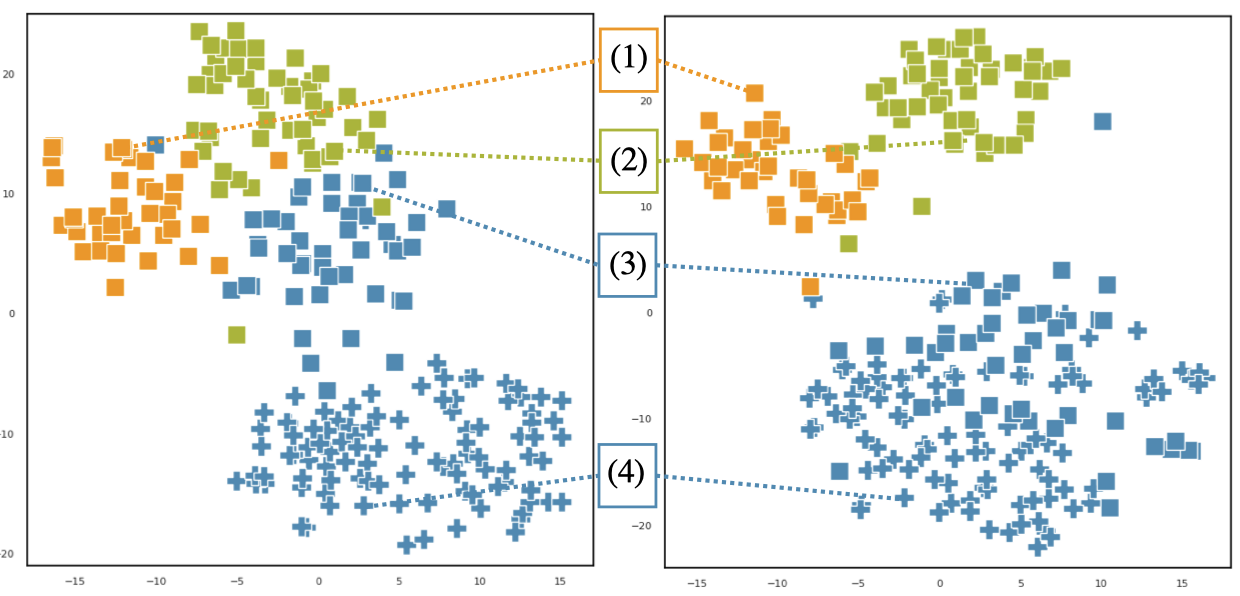
\includegraphics[width=\textwidth]{figures/media/image7.png}
  \caption{\label{fig:bert}Figure 1 aus Yamada et al. \autocite*[811]{yamadaSemanticFrameInduction2021}. Originale Bildunterschrift: \emph{2D projections of BERT embeddings of verbs (left) and masked verbs (right). Numbers in the figure correspond to numbers in Table 1,} ⬛ \emph{and \textbf{+} are verbs ``get'' and ``acquire'', respectively, and each color indicates \textcolor[RGB]{234,151,44}{ARRIVING}, \textcolor[RGB]{170,181,61}{TRANSITION\_TO\_STATE}, and \textcolor[RGB]{81,137,177}{GETTING} frame.}}
\end{figure}

Mithilfe des Language Models BERT \autocite{devlinBERTPretrainingDeep2019} können sie für jedes Verb in diesen Sätzen eine kontextualisierte Vektor-Repräsentation erzeugen. Im Gegensatz zu klassischen Word Embeddings (\chapref{word-embeddings-als-paradigmatische-distributionelle-muster}) erhalten sie so ein Embedding pro Token und nicht pro Type und können unterschiedliche Verbbedeutungen und mithin unterschiedliche LE potenziell unterscheiden. \figref{fig:bert} zeigt die Verbesserung, die sie erreichen, indem sie BERT das Embedding nicht für das Verb-Token, wie es im Satz steht, erzeugen lassen, sondern es zuvor maskieren, sodass das Sprachmodell keine Information darüber erhält, welches Wort an der Stelle eigentlich steht. Es wird also z.\,B. ein Embedding für die maskierte Stelle im Satz \emph{We'll not} {[}MASK{]} \emph{there before the rain comes} erzeugt. Dem linken Teil der Abbildung ist zu entnehmen, dass in der unmaskierten Variante die Sätze mit den drei Bedeutungen von \emph{get} zwar bereits in unterschiedlichen Clustern zu finden sind, allerdings jeweils durch die identische Formseite auch einander äußerst nah sind. Erst durch die Maskierung, deren Ergebnisse im rechten Teil der Abbildung dargestellt sind, sind Sätze mit \emph{get} in der GETTING-Bedeutung deutlicher separiert und bilden -- zielgemäß -- ein gemeinsames Cluster mit den Sätzen mit \emph{acquire} in der GETTING-Bedeutung. Es liegen des Weiteren Ansätze vor, die FE induzieren und grundsätzlich ähnlich funktionieren, wobei aber auch syntaktische Dependenzbeziehungen der Verben zu ihren Argumenten einbezogen werden \autocite[z.\,B.][]{anwarHHMMSemEval2019Task2019}.

Word Embeddings beruhen auf paradigmatischer distributioneller Ähnlichkeit, d.\,h. Wörter mit ähnlichen Kotexten erhalten ähnliche Vektorrepräsentationen und sind mithin in gleichen Clustern zu finden. Die Embedding-basierten Ansätze zur Frame-Induktion greifen also auf distributionelle Eigenschaften von Sprache zurück, um sie Frames zuzuordnen. Gemäß der Ausrichtung von \emph{FrameNet} sind auch die Frame-induzierenden Ansätze in aller Regel an Verben interessiert und teilen mithin das Defizit der Fillmoreschen Frame-Semantik, den konzeptuellen Gehalt von (u.\,a.) Nomen und Adjektiven zu vernachlässigen (\chapref{welche-frames-werden-aufgenommen} und \ref{warum-frames}). Auch beschränken sie sich weitestgehend auf die Zuordnung von Verben zu bestehenden \emph{FrameNet}-Frames, anstatt wirklich neue Frames zu erschließen und deren FE zu beschreiben.

\subsection{Distributionell-semantische Methodik}\label{distributionell-semantische-methodik}

In korpuslinguistischen Zugängen hat sich eine Reihe distributioneller Methoden etabliert, um die Semantik sprachlicher Einheiten von der Wort- bis zur Textebene zu erfassen. Die wohl etabliertesten und insbesondere auch im Bereich der englischsprachigen CADS viel genutzten Verfahren sind die Kollokations- und die Keyword-Analyse.\footnote{Siehe dazu etwa Gillings et al. (2023: 2), die diese zusammen mit Frequenz- und Konkordanz-Analyse als „the four main corpus tools`` listen.} Die Idee der Kollokationsanalyse ist in \chapref{distributionelle-semantik} bereits umrissen worden und wird in \chapref{kollokationen-als-syntagmatische-distributionelle-muster} näher in ihrer Funktionsweise erläutert. Es geht bei ihr darum, die Semantik eines Wortes und seine Gebrauchsprofile in einzelnen Diskursen über das statistisch signifikant häufige Ko-Vorkommen mit anderen Wörtern zu erschließen. Zur Messung der statistischen Signifikanz können dabei unterschiedliche Maße zum Einsatz kommen, die je unterschiedliche Ergebnisse produzieren (siehe \chapref{wie-funktioniert-die-berechnung-von-kollokationen}). Baker etwa stellt in Bezug auf vorherige Untersuchungsergebnisse \autocite{bakerDiscourseAnalysisMedia2013} heraus, dass das Adjektiv \emph{muslim} in der britischen Presse insbesondere in Bezug auf islamistische Akteure genutzt wird:

\begin{quote}
We found that one common pattern in this context concerned words relating to extreme belief, such as \emph{extremist}(\emph{s}), \emph{fundamentalist}(\emph{s}) and \emph{militant}(\emph{s}). Such words also were common when Muslim was a noun, and they also occurred frequently with two other high-frequency words \emph{Islam} and \emph{Islamic}. \autocite[248]{bakerAcceptableBiasUsing2012}
\end{quote}

In einer vertiefenden Analyse zeigt er außerdem, dass sie weitaus häufiger gebraucht werden als Wörter, die einen strengen, aber nicht extremistischen oder moderaten Glauben anzeigen (Baker 2012: 251--252), was auf einer in diesen Ansätzen häufig vorgenommenen Kategorisierung der Kollokate nach semantischen Gesichtspunkten beruht. Zur Analyse von Framing arbeiten auch Czulo et al. \autocite*{czuloEinflussExtremistischerGewaltereignisse2020} mit Kollokationen (siehe \chapref{weitere-arbeiten-zum-extremismusdiskurs-und--begriff}). Für eine Übersicht über die zahllosen weiteren Anwendungen von Kollokationsanalysen sei auf den ausführlichen Literaturüberblick bei Storjohann \autocite*{storjohannKookkurrenzAusKorpuslinguistischer2016} verwiesen.

In Bezug auf methodologische Weiterentwicklungen ist die besonders raffinierte Version der Kollokations-Analyse von Belica zu nennen. Sie ist über die Kookkurrenzdatenbank CCDB am IDS-Mannheim \autocite{belicaKookkurrenzdatenbankCCDBKorpuslinguistische2001} zugänglich und listet neben den unmittelbaren Kollokaten rekursiv auch deren Kollokate sowie typische syntagmatische Muster. Für die Analyse von Konstruktions-Fillern in der Konstruktionsgrammatik ist die von Stefanowitsch \& Gries \autocite*{stefanowitschCollostructionsInvestigatingInteraction2003} entwickelte und ebenfalls auf Kollokationen beruhende Kollostruktionsanalyse einschlägig, mit deren Hilfe sich etwa \emph{give}, \emph{tell} und \emph{send} als typische Filler des Verb-Slots der \emph{ditransitive construction} identifizieren lassen \autocite[229, Table 10]{stefanowitschCollostructionsInvestigatingInteraction2003}, was gemäß distributionell-semantischer Annahmen eine wichtige Dimension von Konstruktionsbedeutungen darstellt \autocite{ziemDimensionsConstructionalMeanings2023}. Eine andere Weiterentwicklung stellt die Berechnung und Visualisierung ganzer Kollokationsnetzwerke dar, in denen auch gegenseitige Abhängigkeiten der Kollokate eines Wortes in Form eines Netzwerk-Graphen dargestellt sind. Brezina et al. heben zum einen ihren zusammenfassenden Charakter und den Zugang zur „psychological notion of the `aboutness' of a text`` \autocite*[142]{brezinaCollocationsContextNew2015} im Sinne von Phillips \autocite*{phillipsLexicalStructureText1989} hervor, gehen aber auch auf ihr Potenzial ein, komplexe diskursive Bedeutungszusammenhänge zu erkennen, u.\,a. am Beispiel des \emph{swearing discourse}:

\begin{quote}
To appreciate the complexity of the moralistic discourse we also need to look at how the immediate associations are connected with one another and, more importantly, how these are connected to other (more distant) associations. Thus, for instance, in 17th and 18th century discourse, \emph{swearing} is connected with a whole range of religious evaluations, through further associations of vice with notions such as \emph{prophaneness} and \emph{irreligion} {[}\ldots{]}. Ultimately, any discourse rests upon a large network of associations, where each one activates a number of others (cf. Hoey 2005), that produces social meaning through multiple cross-associations. These cross-associations, however, cannot be observed even with careful reading of source documents, but need to be analysed using a tool that allows simultaneous multiple comparisons of word frequencies and co-occurrences. \autocite[155]{brezinaCollocationsContextNew2015}
\end{quote}

Die Visualisierung hat darüber hinaus auch schlicht den Vorteil, eine lange Liste von Kollokationsbeziehungen in einem Korpus überhaupt überblicken zu können:

\begin{quote}
Es ist unmöglich, durch Lesen solcher langer Listen einen Eindruck über das Ensemble der Verknüpfungen zu erhalten. Erst durch die Visualisierung als Netz kann sich ein Bild ergeben (Pfeffer 2010; für einen historischen Blick auf Visualisierungen von Netzwerken: Kruja et al. 2002). \autocite[231]{bubenhofer9DiskurslinguistikUnd2018}
\end{quote}

Letztlich sei auf Bakers Arbeit verwiesen, die das Potenzial von Kollokationsnetzwerken hervorhebt, u.\,a. bedeutungsäquivalente Wörter zu erkennen, und zwar dadurch dass sie ähnliche Kollokate aufweisen, ohne zwingend gemeinsam aufzutreten \autocite*[147-148]{bakerShapesCollocation2016} -- ein Befund also, der sich vor dem Hintergrund distributionell-semantischer Annahmen bestens erklären lässt und auch der Idee von Word Embeddings (s.u.) zugrundeliegt.

Keyword-Analysen (dt. auch Schlüssel- oder Schlagwortanalysen) sind im Gegensatz zu Kollokationsanalysen eine \emph{corpus-driven} und kontrastive Methode, die Wörter\footnote{Statt einzelner Wörter können natürlich auch Mehrworteinheiten bzw. Sprachgebrauchsmuster oder einzelne Annotationen in Hinblick auf ihre Keyness bewertet werden \autocite{bubenhoferSprachgebrauchsmusterKorpuslinguistikAls2009, bubenhofer4KollokationenNGramme2017}.} zu Tage fördert, die in einem Korpus signifikant häufiger gebraucht werden als in einem anderen Korpus. Sie dienen so dazu, die \emph{aboutness} eines Korpus zu erschließen \autocite{gabrielatosKeynessAnalysisNature2018} und wurden auch bereits bei der Analyse von kommunikationswissenschatlichem Framing \autocite{bakerChangingFramesObesity2020} sowie in Frame-semantischen Ansätzen \autocite{ziemMedienFramesAlsSemantische2018} eingesetzt. Eine Nutzung von Keywords als Features in multiplen Korrespondenzanalysen wurde von Clarke et al. vorgeschlagen \autocite{clarkeMultipleCorrespondenceAnalysis2021, clarkeKeywordsTimeTracking2022}. Während bei der Kontrastierung nach z.\,B. diachronen oder akteursbezogenen Kriterien\footnote{Nur beispielhaft genannt seien Bubenhofer \autocite*{bubenhofer4KollokationenNGramme2017}, der den Nutzen der Methode zur Analyse des typischen Wortschatzes einzelner Parteien vorführt und Clarke et al. \autocite*{clarkeKeywordsTimeTracking2022}, die diachrone Unterschiede im Islamdiskurs fokussieren.} unstrittige Metadaten zur Bildung der zu vergleichenden Korpora genutzt werden können, erfordert der Vergleich einzelner thematischer Diskurse die voraussetzungsreichere Bildung entsprechender virtueller Diskurskorpora \autocite{busseIstDiskursSprachwissenschaftliches1994}. Dies geschieht in der Korpuslinguistik zumeist durch die Festlegung einzelner repräsentativer Suchwörter, wobei nur die Texte, die diese Wörter enthalten, in das Korpus aufgenommen werden. Dieser Schritt ist jedoch durchaus kritisch, da so -- Frame-semantisch gesprochen -- bereits vorausgesetzt wird, welche LE einen thematischen Frame evozieren. Genau das soll ja aber auch das Ergebnis der Analyse sein. So könnte, wer ein Diskurskorpus zum Islamismus zusammenstellt und dafür das Lemma \emph{islamistisch} verwendet, Texte verpassen, in denen -- wie diskurslinguistisch bereits mehrfach herausgestellt -- regelmäßig nicht von ‚Islamisten`, sondern z.\,B. \emph{muslimischen Extremisten} \autocite[116, Tabelle 23]{kalwaKonzeptIslamDiskurslinguistische2013} oder \emph{fanatic Muslims} \autocite[249, Table 1]{bakerAcceptableBiasUsing2012} die Rede ist. Natürlich ist es wahrscheinlich, dass in vielen Texten, in denen von \emph{muslimischen Extremisten} die Rede ist, \emph{auch} das Wort \emph{islamistisch} vorkommt, was das Problem deutlich mindert. Und auch bei der Untersuchung thematisch eng gefasster Diskurse wie der Snowden-Affäre \autocite{ziemMedienFramesAlsSemantische2018} oder der frühen Corona-Pandemie \autocite{bubenhoferGrenzenUndWelten2020} ist es unwahrscheinlich, dass die zugrundegelegten \emph{seed words} (\emph{Snowden}, \emph{NSA}, \emph{data} bzw. \emph{Corona}) nicht in den Texten vorkommen. Für den in der vorliegenden Arbeit zu untersuchenden Extremismus-Diskurs, bei dem begriffliche Verwirrungen und Unsicherheiten fortwährender Gegenstand der wissenschaftlichen Debatte sind und für den im Untersuchungszeitraum eine geradezu unzählige Menge relevanter Ereignisse und Akteure zu berücksichtigen gelten würde, kommt ein solches Vorgehen und mithin Keyword-Analysen nicht in Frage. Stattdessen soll nach Möglichkeiten gesucht werden, auch in einem thematisch heterogenen Korpus einzelne Diskurse bzw. thematische Frames datengeleitet aufzuspüren.

Neben diesen etablierten Methoden haben auch neuere, aus der Computerlinguistik stammende Verfahren Anwendung in diskursanalytischen Arbeiten gefunden. Zum einen ist hier Topic Modelling \autocite{bleiLatentDirichletAllocation2003} zu nennen, mit dessen Hilfe für jedes Wort und jeden Text (\emph{document}) in einem Korpus bestimmt werden kann, mit welcher Wahrscheinlichkeit es zu einem \emph{topic} gehört. Zugrunde liegt ebenfalls die Verteilung von Wörtern über die \emph{documents} des Korpus, wobei jedes einzelne \emph{document} als sogenannte \emph{bag of words} aufgefasst wird, sodass die syntagmatische Nähe bzw. Abfolge der Wörter keine Rolle spielt. Die \emph{topics} werden durch Listen von Wörtern dargestellt. So finden etwa Bubenhofer et al. \autocite*[82]{bubenhoferDigitaleKulturlinguistikDigitalitaet2022} in Rezepten der Plattform Chefkoch ein \emph{topic} mit Wörtern wie \emph{leider}, \emph{zwar}, \emph{überhaupt} und \emph{irgendwie}, das sie als Bewertungen und Positionierungen interpretieren. Weiterhin angewendet wurde Topic Modeling in der Diskurslinguistik z.\,B. bei Törnberg \& Törnberg \autocite*{tornbergMuslimsSocialMedia2016}, Murakami et al. \autocite*{murakamiWhatThisCorpus2017}, Bubenhofer et al. \autocite*{bubenhoferGrenzenUndWelten2020} oder Dreesen et al. \autocite*{dreesenOperationalisierungDiskurslinguistischenKategorie2023}; kritisch reflektiert in den Arbeiten von Brookes \& McEnery \autocite*{brookesUtilityTopicModelling2019} sowie Gillings \& Hardie \autocite*{gillingsInterpretationTopicModels2023}. Da Topic Modeling durchaus interessante Möglichkeiten für \emph{corpus-driven} Ansätze eröffnet, wurde auch bei der Methodenentwicklung in diesem Projekt mit dem Verfahren experimentiert; die Anforderungen an den Arbeitsspeicher überstiegen jedoch aufgrund des sehr großen Korpus die zur Verfügung stehenden Möglichkeiten. Des Weiteren liegt das eigentliche Ziel des Verfahrens, die thematische Klassifikation von Texten, nicht im Untersuchungsinteresse; die Modellierung und das Clustering einzelner Wortbedeutungen wiederum ist hingegen besser durch die computerlinguistische Methodengruppe der Word Embeddings zu realisieren.

Wie bereits erwähnt, ist es mithilfe von Word-Embedding-Algorithmen möglich, Wörter auf der Grundlage ihrer Distribution in Korpora in Vektoren zu überführen. Die Nähe und Distanz im sich ergebenden Vektorraum entspricht dabei einer paradigmatischen distributionellen Ähnlichkeit; benachbarte Wörter haben ähnliche Kotexte (siehe ausführlicher \chapref{distributionelle-semantik} und \ref{word-embeddings-als-paradigmatische-distributionelle-muster}). Große Popularität gewonnen haben solche Ansätze mit der Verbreitung der Nutzung neuronaler Netze, die die ressourceneffiziente Berechnung von Word Embeddings für große Korpora erlaubte \autocite{mikolovEfficientEstimationWord2013}. In der Diskurslinguistik spielt bislang insbesondere die Analyse lokaler Nachbarschaften im Vektorraum eine Rolle, die semantisch-funktionale Äquivalenz widerspiegelt \autocite{bubenhoferSemantischeAquivalenzGeburtserzahlungen2020}. In diesem Rahmen können auch Clustering-Algorithmen wie \emph{k-Means} \autocite{macqueenMethodsClassificationAnalysis1967} zum Einsatz kommen, die solche Nachbarschaften automatisiert erkennen (siehe \chapref{clustering-von-word-embeddings}). Bubenhofer zeigt so etwa, dass ein Wort-Cluster um die (Mehrwort\mbox{-})Lemmata \emph{demokratisch Staat}, \emph{zentralistisch} und \emph{totalitär Regime} während der Corona-Pandemie deutlich häufiger durch rechte und Corona-skeptische Medien wie u.\,a. Compact Online und KenFM.de gebraucht wurde:

\begin{quote}
Die Verteilung über die Quellen in Abbildung 2 zeigt nun deutlich, dass Ausdrücke des Clusters in den Skep-Medien deutlich häufiger verwendet werden. Die Kommentare (mit Ausnahme von 20 Minuten) liegen zusammen mit den CH-Medien NZZ und Tages-Anzeiger dazwischen. In den restlichen Quellen werden die Ausdrücke des Clusters seltener verwendet. Es muss berücksichtigt werden, dass mit \emph{demokratisch} und \emph{regieren} zwei Ausdrücke im Cluster vorhanden sind, die hinsichtlich eines politischen Standpunktes (in einer Demokratie) unauffällig sind. Die meisten der restlichen Ausdrücke jedoch sind Stigmawörter (Spitzmüller/ Warnke 2011, S. 143) und kritisieren im Kontext der Corona-Pandemie die angeblich totalitäre Ausrichtung des Staates. {[}\ldots{]} Auch die Cluster 843 (\emph{Diktatur}, \emph{Polizeistaat}, \emph{totalitär Staat}) und 1731 (\emph{Ungehorsam}, \emph{Gesundheitsdiktatur}, \emph{Repression}) enthalten Stigmawörter für den Staat und werden in den Skep-Medien häufiger verwendet als in den anderen Quellen. \autocite[205-206]{bubenhoferExplorationSemantischerRaeume2022}
\end{quote}

Das Clustering und die Analyse der Frequenz-Unterschiede in unterschiedlichen Medien können also ohne die Notwendigkeit von händischen Annotationen Charakteristika des Sprachgebrauchs einzelner medialer Akteure freilegen. Weiterhin analysiert Bubenhofer, wie zuvor in Zusammenarbeit mit Calleri und Dreesen \autocite*{bubenhoferPolitisierungRechtspopulistischenMedien2019}, divergierende Semantisierungen einzelner Wörter im Vergleich der Korpora. Da die Vektoren von auf unterschiedlichen Korpora berechneten Word-Embedding-Modellen nicht unmittelbar vergleichbar sind (siehe \chapref{vergleichbarkeit-von-word-embedding-modellen}), werden dabei nicht die Vektoren selbst verglichen, sondern ihre lexikalischen Nachbarn im Vektorraum. Einen deutlichen Unterschied stellt er u.\,a. beim Ausdruck \emph{Narrativ} fest:

\begin{quote}
In den beiden Modellen sind nur \emph{Halbwahrheit}, \emph{instrumentalisiert}, \emph{Massenmedium}, \emph{Populismus} und \emph{Verschwörung} semantisch ähnliche Ausdrücke, die in beiden Modellen vorkommen. Ansonsten unterscheiden sich die Modelle deutlich. Nächste Nachbarn wie \emph{Angsterzeugung}, \emph{aufbauschen}, \emph{böse Absicht}, \emph{dahinter stecken}, \emph{Fiktion}, \emph{infam}, \emph{Inszenierung}, \emph{krampfhaft}, \emph{Leugnung}, \emph{Lügenpropaganda}, \emph{Massenpsychologie}, \emph{psychologische} Kriegsführung, \emph{Unwahrheit}, \emph{Wahn} oder \emph{Weltverschwörung} zeichnen einen semantischen Raum, bei dem \emph{Narrativ} als bösartige Manipulation semantisiert ist. Im CH-Medien-Korpus gibt es ebenfalls Ausdrücke, die diese Semantisierung nahelegen, jedoch auch andere wie \emph{westliche Demokratie}, \emph{Ideologie}, \emph{Deutungshoheit} oder \emph{politische Debatte}, die der sozialwissenschaftlichen Definition von Narrativ als sinnstiftende Erzählung näher kommen (Lyotard 2015). \autocite[214]{bubenhoferExplorationSemantischerRaeume2022}
\end{quote}

Dass in Word Embeddings weit mehr als eine globale semantisch-funktionale Ähnlichkeit gespeichert ist, zeigen Kozlowski et al. \autocite*{kozlowskiGeometryCultureAnalyzing2019}. In einer aufwändigen diskursanalytischen Untersuchung zum Konzept \emph{class} nutzen sie Antonympaare wie \emph{poor} und \emph{rich} oder \emph{masculine} und \emph{feminine}, um semantische Achsen im Vektorraum aufzuspannen. Sie können so unterschiedliche in der Literatur beschriebene Dimensionen des Konzeptes wie ‚Wohlstand`, ‚\emph{race}` oder ‚Gender` operationalisieren und diachrone diskursive Veränderungen vermessen. \figref{fig:kozlowski} zeigt exemplarisch, wie so einzelne Sportarten in Hinblick auf diese Dimensionen verortet werden können. Dass solche vektorgeometrischen Berechnungen nicht nur dem Anschein nach plausibel Auskunft über in Diskursen manifestierte Stereotype geben, sondern tatsächlich eng mit Sprecher*innen-Urteilen korrelieren, belegen sie durch eine Fragebogenstudie \autocite[siehe auch aus kognitionswissenschaftler Perspektive][]{grandSemanticProjectionRecovers2022}.

\largerpage
\begin{figure}[b]
\includegraphics[width=.7\textwidth]{figures/media/kozlowski-cropped.png}
  \caption{\label{fig:kozlowski}Semantische Projektion der Wortvektoren unterschiedlicher Sportarten auf zwei ‚kulturelle Dimensionen` (eigene Visualisierung von \emph{Figure} 2c aus \citealt[913]{kozlowskiGeometryCultureAnalyzing2019}).}
\end{figure}

Für kulturwissenschaftliche Fragestellungen bedeutet dies nicht weniger als die Möglichkeit, die Intersektionalität unterschiedlicher kultureller Dimensionen modellieren zu können:

\newpage
\begin{quote}
The ability of word embedding models to simultaneously locate objects on multiple cultural dimensions, including race, gender, class, and many others, makes them a powerful tool for studies of intersectionality. The fundamental insight of the intersectionality literature is that cultural categories, particularly those of identity, cannot be isolated and understood independently (Crenshaw 1991; McCall 2005). Rather, analysts must always consider ways in which the meanings of cultural categories change as they overlap and intersect one another. Interrogation of the intersection of cultural categories becomes empirically tractable through word embedding models. For example, comparing words that project high on both affluence and masculinity to those that project high on affluence and femininity will reveal how markers of class differ across gender lines within the cultural world in which the texts were produced. The theory that identity is defined by numerous crosscutting and overlapping categories is itself predicated on a ``high-dimensional'' model of culture similar to that modeled by Euclidean word embeddings. Indeed, the empirical success of word embedding models to represent cultural dimensions promotes a radical view of intersectional identity, modeled not as a low-dimensional matrix, but rather a highdimensional array composed of hundreds or thousands of interacting cultural associations. \autocite[914-915]{kozlowskiGeometryCultureAnalyzing2019}
\end{quote}

Auch linguistische Ansätze, in denen einzelne sprachliche Einheiten semantisch gruppiert werden sollen, profitieren von der Möglichkeit einer induktiven und hochdimensionalen Modellierung von Wortbedeutungen. So weiß jede*r, der*die entsprechende Annotationen schon einmal händisch durchgeführt hat, dass man ständig Zweifelsfällen begegnet, in denen ein Wort -- womöglich in Abhängigkeit des konkreten jeweiligen Kontextes -- in verschiedene Kategorien gezählt werden könnte. Letztlich ist man jedoch, um die Komplexität beherrschbar zu halten und auch um ein Agreement mit den anderen Annotator*innen zu erreichen, i.d.R. gezwungen, sich auf eine Möglichkeit festzulegen. Es wäre ja andernfalls auch notwendig, die Zugehörigkeit zu den unterschiedlichen Kategorien graduell zu quantifizieren, was nur noch in sehr kleinen Untersuchungen zu leisten wäre. Ein Beispiel stellt die Untersuchung von Baker et al. (2020) dar. Sie berichten zunächst, dass sie sich gegen den Einsatz eines (durchaus verbreiteten) semantischen Taggers wie \emph{Wmatrix} \autocite{raysonKeyWordsKey2008} entschieden haben, der Wörter im Wesentlich auf Basis eines statischen Thesaurus in Kategorien einordnet. Stattdessen, insbesondere um kontextuelle Faktoren besser berücksichtigen zu können, entscheiden sie sich für eine induktive manuelle Kategorisierung von Keywords:

\begin{quote}
Automatic taggers do not always recognise every word they encounter and often assign categories based on surface meaning, whereas it can be more useful to take into account the contexts in which the words are used. For example, one of the categories we created was ILLNESS, which contained words like \emph{cancer}, \emph{diabetes} and \emph{inflammation}. We included words like~\emph{heart}~and~\emph{liver}~in this category, as our explorations of how those words occurred in the context of articles revealed that they almost always referred to heart or liver disease. However, we did not categorise the word~\emph{epidemic}~as ILLNESS, as instead we found it was almost always used metaphorically to refer to purported increases in rates of obesity, for example:

\begin{quote}
High~sugar consumption~is said to be fuelling the obesity epidemic, which is leading to increased cases of~heart disease. (\emph{Daily Mail}, April 2009)
\end{quote}

Thus, we created a category called PROBLEM and included~\emph{epidemic}~alongside words such as~\emph{risk},~\emph{crisis}~and~\emph{problem}, as all four words were used to frame obesity in a negative way. Categorisation was carried out separately by two of the authors at first and then jointly to resolve a small number of disagreements. We should note that we did not speculate about how the keywords in our data were used in order to categorise them. Rather, we closely analysed at least 100 random cases of each of the words to resolve them into categories that best reflected their most typical use (this was a method first adopted in Baker et al. (2019), based on experimenting with different numbers of cases in order to identify an amount which was most effective at identifying the range of contexts that a word can occur in). Where a word had more than one meaning and could appear in multiple categories, we chose the meaning which was most frequent out of the 100 random cases examined. Not all words could be easily assigned to a category as they had a range of frequent meanings or were used in ambiguous ways. For this reason, we did not categorise 131 of the keywords. \autocite[4]{bakerChangingFramesObesity2020}
\end{quote}

Hier ist m.\,E. durchaus fraglich, warum die als Beispiel angeführte „obesity pandemic`` nicht sowohl einen semantischen Bezug zum Bereich „PROBLEM`` als auch zum Bereich „ILLNESS`` aufweisen sollte. Und auch das Ansinnen, in einem aufwändigen Verfahren dominante Bedeutungen von Wörtern aus Konkordanzsamples zu erschließen, um eindeutige Annotationen vornehmen zu können bzw. ambige Wörter dabei auszuschließen, wird der tatsächlichen Komplexität von Semantik m.\,E. nicht gerecht. Natürlich kann der Schritt aus forschungspraktischen Gründen vollkommen gerechtfertigt sein und keine Untersuchung kommt ohne Vereinfachungen aus -- umso potenzialreicher erscheint jedoch die Möglichkeit einer hochdimensionalen Bedeutungsmodellierung mithilfe von Word Embeddings. So resümieren auch Kozlowski et al.:

\begin{quote}
The very success of these models provides suggestive validation for relational approaches to cultural theorizing. Furthermore, by operationalizing a high dimensional model of culture, word embedding models allow researchers to extend and contend with theories of culture in novel ways. Embeddings present a much vaster set of potential axes along which individuals and social groups may compete, cooperate, fracture, or coalesce than low-dimension theories of cultural constraint allow. By simultaneously capturing the multiplicity of associations expressed in language, word embedding models are able to represent a complex geometry of culture, which, like a many-faceted crystal, amplifies the subtle and shifting framings that enable coordinated and spontaneous social action. \autocite[931]{kozlowskiGeometryCultureAnalyzing2019}
\end{quote}

Eine Kombination von syntagmatischen und paradigmatischen Methoden für diskurssemantische Fragestellungen schlagen Vachková \& Belica \autocite*{vachkovaSelfOrganizingLexicalFeature2008} unter Nutzung der von Belica \autocite*{belicaKookkurrenzdatenbankCCDBKorpuslinguistische2001, belicaSemantischeNaheAls2011} für die Linguistik adaptierten Methode der s\emph{elf-organizing lexical feature maps} \autocite[SOM;][]{kohonenSelfOrganizingMaps2001} vor. Dabei wird die syntagmatische Kollokationsanalyse mit einer paradigmatischen Analyse geteilter Kollokationsprofile der Kollokate gepaart. \figref{fig:som-tod} zeigt ein Beispiel.

\begin{figure}[t]
  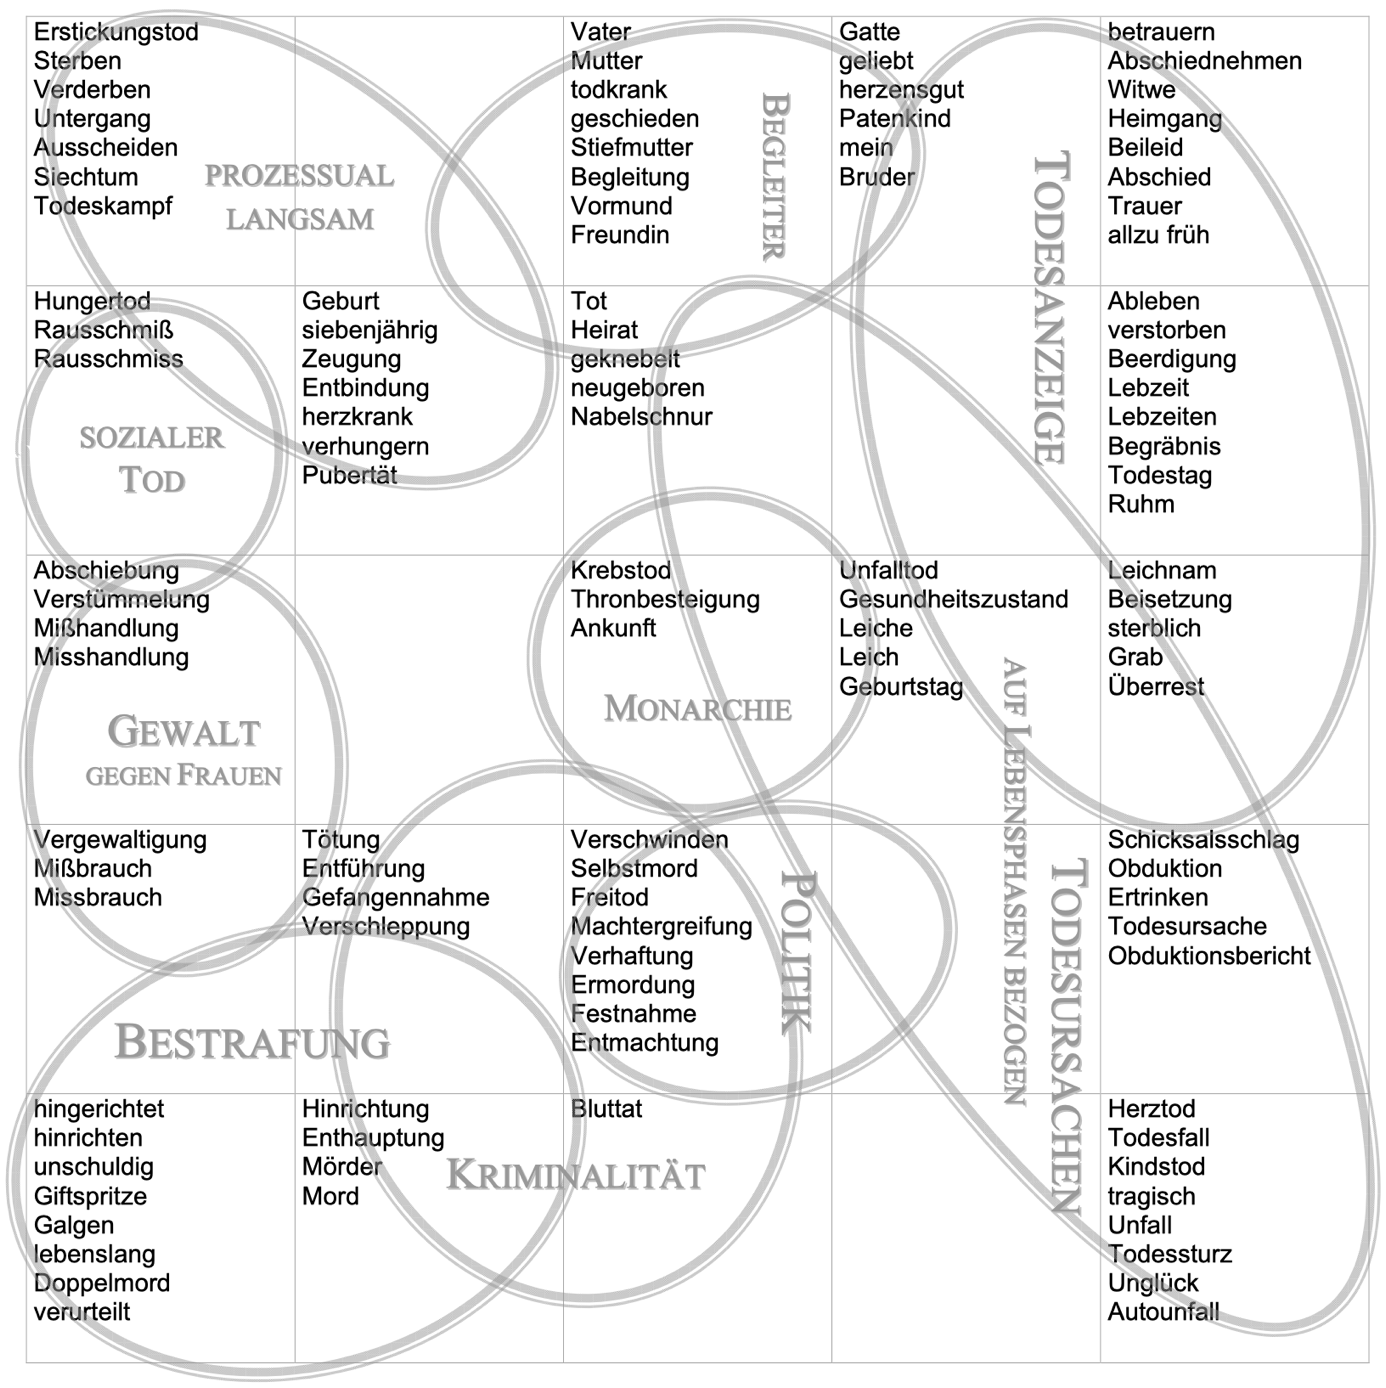
\includegraphics[width=\textwidth]{figures/media/image9.png}
  \caption{\label{fig:som-tod}Annotierte SOM zu \emph{Tod} (\emph{Figure 3} aus \citealt[250-251]{vachkovaSelfOrganizingLexicalFeature2008}).}
\end{figure}

In den einzelnen Quadraten sind jeweils Kollokate zum Wort \emph{Tod} dargestellt. Die Kollokate werden jedoch zusätzlich geclustert, sodass Kollokate, die selbst wiederum ähnliche Kollokationsprofile aufweisen, miteinander in einem Quadrat zu finden sind. Die sich ergebenden Cluster sind sodann interpretierbar und zeigen etwa den Trauer-Aspekt von Tod (u.\,a. \emph{betrauern}, \emph{Abschiednehmen}, \emph{Witwe}) oder den Kriminalitäts- bzw. Bestrafungs-Aspekt in jeweils grausamer Ausprägung an (u.\,a. \emph{Bluttat}, \emph{Hinrichtung}, \emph{Enthauptung}). Die Autor*innen konstatieren:

\begin{quote}
We suggest that the proposed approach of self-organizing clustering of collocation profiles extracted from very large text corpora followed by a discourse-based semiotic interpretation and a deferred mapping of the emergent signs to systemic linguistic categories is a coherent and adequate methodology for the explorative study of language. We argue that the epistemic results obtained by applying this methodology also entail predictive and explanatory power. \autocite[238-239]{vachkovaSelfOrganizingLexicalFeature2008}
\end{quote}

Fragt man in der CCDB die SOM zum Lemma \emph{Extremismus} ab, findet sich einerseits ein Cluster wie {[}\emph{Nährboden}, \emph{Separatismus}, \emph{Terror}, \emph{Anwachs}, \emph{Anwachsen}, \emph{Gedankengut}, \emph{rassistisch}, \emph{Hetze}{]}, das die ideologische, im Verborgenen anwachsende Gefahr von extremistischem Gedankengut anzeigt; andererseits ein Cluster wie {[}\emph{Rassismus}, \emph{Fremdenfeindlichkeit}, \emph{Ausländerfeindlichkeit}, \emph{Fremdenhaß}, \emph{Fremdenhass}, \emph{Ausländerhaß}, \emph{Ausländerhass}, \emph{Ausgrenzung}{]}, das also Rassismus und Xenophobie, d.\,h. im Rechtsextremismus vorzufindende Einstellungen, zusammenfasst. Diese Beobachtung ist von großem Interesse für das Vorhaben einer korpuslinguistischen Untersuchung des Extremismusdiskurses, zeigen sich hier doch wesentliche semantische Dimensionen von Extremismus, die auch als FE eines Extremismus-Frames interpretierbar sind. So bündelt das zweitgenannte Cluster Einstellungen bzw. Motivationen rechtsextremistischer Akteure und enthält zugleich LE, die dieses FE evozieren. Es zeichnen sich in einer solchen Kombination distributioneller Verfahren, die im Fall der SOM noch limitiert und auf die Analyse einer vorberechneten Menge von Lemmata begrenzt ist, also sehr vielversprechende Potenziale für eine korpuslinguistische Frame-Modellierung ab, die es weiter zu prüfen gilt.

\section{Resümee}\label{resuemee}

\subsection{Warum Frames?}\label{warum-frames}

Vor dem Hintergrund der dargelegten theoretischen Grundlagen soll im Folgenden noch einmal zusammengefasst werden, warum gerade Frames ein geeignetes Modell diskursiven Wissens darstellen, um diskursive Unterschiede im Framing von Extremismus zu analysieren. Es wird auch darauf eingegangen, warum dabei die Entscheidung für Busses Frame-Modell anstatt des verbreiteteren \emph{FrameNet}-Ansatzes getroffen wurde. Im Anschluss wird skizziert, warum distributionell-semantische Ansätze ein geeignetes Mittel sind, um Frames induktiv zu erschließen und welche genauen Verfahren für die sich anschließende Methodenentwicklung einbezogen werden. Letztlich sollen inhaltliche Mindestbestandteile eines Extremismus-Frames resümiert werden, um eine orientierende Grundlage für die datengeleitete Analyse zu schaffen.

Als Vorzug eines Frame-semantischen Modells für die Diskursanalyse ist erstens zu nennen, dass es die Bedeutungskomplexität einzelner Begriffe überhaupt erfassen und modellieren kann. So Busse zum Bereich der politischen Lexik:

\begin{quote}
Ein Wort wie \emph{Steuererleichterung} thematisiert das Leiden unter einer Last, \emph{Todessteuer} statt \emph{Erbschaftssteuer} evoziert „das unwillkommene Bild, für das Sterben bestraft zu werden`` und \emph{das kleine Baby} statt \emph{Fötus} evoziert die Assoziation „eines kleinen und hilflosen menschlichen Wesens, das des Schutzes bedarf`` (Fillmore 2006, 620). Solche Bedeutungselemente oder verstehensrelevanten Wissenselemente) können mit klassischen Mitteln und Modellen der linguistischen Semantik gar nicht erfasst werden. Gerade hier zeigt ein frame-analytisches Modell seine besondere Leistungsfähigkeit. Die politische Lexik kann daher als einer der idealen Gegenständer für einen frame-analytischen Ansatz in der Semantik angesehen werden. \autocite[198]{busse33LexikFrameanalytisch2017}
\end{quote}

Im Vergleich zu sozial- oder kulturwissenschaftlichen epistemologischen Modellen ist die Frame-Semantik außerdem von Beginn an auf die präzise Analyse der Wechselwirkung einzelner sprachlicher Zeichen mit diesen Wissensbeständen ausgerichtet. Dies betrifft sowohl die Möglichkeit, einen Frame im Sinne von Bezeichnungskonkurrenz mit unterschiedlichen Wörtern zu evozieren bzw. zu perspektivieren (siehe die Beispiele im obigen Zitat) als auch die kontrastive Erschließung von Bedeutungskonkurrenz, d.\,h. wenn mit demselben Ausdruck und in Abhängigkeit von z.\,B. einzelnen Akteuren unterschiedliche Frames oder Frame-Anteile evoziert werden (siehe zum strategischen Besetzen von Begriffen Klein 1991). Dass Frames nicht geeignet wären, multiple Verweismöglichkeiten von Ausdrücken auf Konzepte zu modellieren \autocite[13-14]{kalwaKonstitutionKonzeptenDiskursen2019}, trifft also nicht zu -- ganz im Gegenteil ist ja einer der zentralen Gedanken der Frame-Semantik, dass unterschiedliche Wörter den gleichen Frame evozieren und dabei jeweils unterschiedlich perspektivieren (siehe \chapref{entailment-case-grammar-understanding-semantics}). Letztlich ist auch die Visualisierbarkeit von Frames (üblicherweise als Netzwerk-Graph), gerade für explorative \emph{corpus-driven} Zugänge, ein nicht zu unterschätzendes Potenzial. Besonders wertvoll ist dies in kontrastiven Studien (wie der vorliegenden), die diachrone Bedeutungsveränderungen oder mediale Abhängigkeiten des Framings untersuchen, wie auch Busse hervorhebt:

\begin{quote}
Frame-analytische Verfahren und Darstellungsweisen sind nach meiner Auffassung besonders gut geeignet, um Fälle konkurrierenden Sprachgebrauchs zu kontrastieren und die semantischen Differenzen klar und deutlich herauszuarbeiten. Wegen derselben Eigenschaften eignen sie sich auch besonders gut zur Illustrierung von Bedeutungswandel. \autocite[210-211]{busse33LexikFrameanalytisch2017}
\end{quote}

Frame-semantische Modelle eignen sich außerdem hervorragend dazu, den Blick auch auf im Diskurs Ungesagtes zu richten, das in der Diskurslinguistik immer wieder als beachtenswert herausgestellt wurde \autocites[39]{spitzmullerDiskurslinguistikEinfuhrungTheorien2011}{storjohannPrasenzUndAbsenz2013}[sowie die Beiträge in][]{schroterExploringSilenceAbsence2018a}. Dies wird insbesondere sichtbar, wenn eigentlich vorgesehene Slots in einem Frame nicht (mehr) gefüllt werden. So formulieren Ziem et al., dass die ausbleibende Realisierung eines FE einem

\begin{quote}
induktiven Verfahren entgehen würde, da diesem zufolge Frame-Elemente allein auf der Basis des gegebenen sprachlichen Materials ermittelt werden. Gerade nicht realisierte Frame-Elemente können aber analytisch sehr interessant sein, insofern sie auf Wissensaspekte verweisen, die im Diskurs marginalisiert werden. \autocite[164]{ziemMedienFramesAlsSemantische2018}
\end{quote}

Einen Blick auf das Ungesagte kann m.\,E. allerdings nicht nur durch die Nutzung bestehender Ontologien wie \emph{FrameNet} gewonnen werden. Es sollte genauso möglich sein, über Kontrastierung unterschiedlicher induktiv gewonnener Frames entsprechende Leerstellen sichtbar zu machen. Einen ähnlichen Ansatz verfolgen auch Storjohann \& Schröter \autocite*{storjohannPrasenzUndAbsenz2013} und verweisen außerdem auf das Desiderat, Frame-Kategorien mithilfe „korpusgestützt{[}er{]} Analysen zahlreicher ähnlicher und nominaler oder verbaler Bezeichnungen`` \autocite*[206]{storjohannPrasenzUndAbsenz2013} aufzudecken. Dabei äußern sie auch den Bedarf einer korpuslinguistischen Methode, die „semantisch zusammenhängend{[}e{]} Kollokatoren und deren Kontexte nach unterschiedlichen linguistischen oder thematischen Kriterien bündeln`` \autocite[205]{storjohannPrasenzUndAbsenz2013} kann. Durch die Kombination von mithilfe von Word Embeddings semantisch gruppierten Wörtern, die als FE gelesen werden, und der Analyse der Kollokationen dieser Wort-Cluster wird die vorliegende Arbeit einen Beitrag zur Umsetzung des Desiderats leisten.

Letztlich ist zu rechtfertigen, warum die Entscheidung zugunsten Busses Frame-Modell, das laut Wengeler \autocite*[23]{wengelerWarnungVorFraming2022} in diskurs- und politolinguistischen Ansätzen kaum praktikabel sei, getroffen wurde, anstatt auf \emph{FrameNet} zurückzugreifen. Von der theoretischen Anlage her ist hier insbesondere der Fokus von \emph{FrameNet} auf Prädikationen zu nennen. Wie bereits in \chapref{welche-frames-werden-aufgenommen} erwähnt, sind zu fundamentalen und Diskurse der jüngeren Zeit bestimmenden Konzepten wie ‚Krieg`, ‚Frieden`, ‚Pandemie` oder eben ‚Extremismus` schlicht keine Frames verzeichnet.\footnote{Zwar ist es nachvollziehbar, dass in einer auf qualitativer Korpusarbeit beruhenden Ressource wie \emph{FrameNet} nur ein begrenztes Set an Einträgen erstellt werden kann; problematisch ist jedoch, dass die Nutzer*in so nie sicher sein kann, ob ein von ihr nicht vorgefundener Frame nicht angelegt ist, weil er in den Augen der Annotator*innen nicht sinnvoll ist oder weil er schlicht noch nicht erfasst wurde bzw. forschungspraktische Gründe der Aufarbeitung entgegenstehen. Darüber hinaus ist der Nutzen der Ressource natürlich nur noch begrenzt gegeben, wenn im Forschungsprozess fortlaufend neue Proto-Frames erstellt werden müssen, wie mitunter vorgeschlagen (siehe \chapref{welche-frames-werden-aufgenommen}).} Finden sich Frames, sind diese eher auf lexikographische Zwecke ausgerichtet, als auf wirklich komplexe epistemische Modellierungen. Busse konstatiert:

\begin{quote}
Zu Grunde liegt offenbar keine epistemologische Perspektive; vielmehr wird eine syntaktische-satz-semantische Perspektive zugrundegelegt, wonach „dominant`` immer das ist, was die Satz-Struktur bestimmt. Der Dominanz-Begriff ist daher (mehr oder weniger) valenztheoretisch definiert, bzw., wie man auch sagen könnte, prädikations-zentriert. Epistemisch gesehen kann man sich jedoch vorstellen, dass auch durch andere Elemente im Satz evozierte Frames ‚dominant`, wenigstens aber gleichgewichtig mit dem verb- oder prädikats-evozierten Frame sein können. \autocite[153]{busseFrameSemantikKompendium2012}
\end{quote}

Der wohl fundamentalste Einwand gegen die Anwendung in korpuspragmatischen Forschungsvorhaben betrifft m.\,E. jedoch die Kontextvergessenheit von \emph{FrameNet}. Die Ressource ist äußerst statisch und neue Release-Versionen erscheinen nur in mehrjährigen Abständen. Insbesondere im Bereich der LE führt dies dazu, dass diskursive Entwicklungen nicht berücksichtigt werden können. Dass also Ausdrücke wie \emph{die Grünen} vielleicht einmal eine Rolle als radikale AKTEURE in einem Extremismus-Frame spielten, dafür heute jedoch AKTEURE wie die \emph{AfD}, der \emph{IS} oder die \emph{Querdenker-Bewegung} zu berücksichtigen wären sowie dass sich der Wortschatz und dessen Semantisierung je nach Medium und Register deutlich unterscheiden kann, ist in einer auf manueller Korpusarbeit beruhenden Ressource nicht widerzuspiegeln, selbst wenn dies im Interesse liegen würde \autocite[siehe aber zu Ansätzen zur Automation z.\,B.][]{anwarGeneratingLexicalRepresentations2020}. Ebenfalls wird die Abbildung rekursiver Frame-Strukturen, dass also auch FE Frames sind, in \emph{FrameNet} nicht realisiert, gleichwohl sie in wichtigen Frame-Theorien vorgesehen (etwa bei Barsalou, Minsky und Busse) und m.\,E. zu berücksichtigen ist. Auch dies ist aufgrund der sich ergebenden Komplexität mit händischer Arbeit nicht umfassend zu realisieren, kann aber in computergestützten Verfahren umgesetzt werden, etwa in Kollokationsnetzwerken.

\subsection{Distributionell-semantische Modellierbarkeit von Frames}\label{distributionell-semantische-modellierbarkeit-von-frames}

Busse et al. \autocite*{busseBedeutungsUndBegriffswissen2018} legen ihrer Frame-semantischen Analyse von Rechtsbegriffen dezidiert keine konkrete Methode zugrunde; Busse positioniert sich außerdem äußerst kritisch gegenüber korpuslinguistischen datengeleiteten Ansätzen (siehe \chapref{frame-induktion}). Meines Erachtens haben distributionell-semantische Ansätze jedoch äußerst große Potenziale für die Induktion von Frames. Sie sollten dabei nicht nur als bloße Mittel zur zusätzlichen Legitimierung gesehen werden,\footnote{So fragen etwa Scholz \& Ziem \autocite*[282]{scholzVokabularImDiskurshistorischen2015} danach, „wie korpuslinguistische Methoden und Werkzeuge als Explorationsinstrumente für große Textdatensammlungen eingesetzt werden können, um die Auswahl von bestimmten Korpusteilen und Textfragmenten mit qualitativen Methoden besser begründen und für inhaltliche, d.\,h. insbesondere diskurssemantische Detailanalysen verfügbar machen zu können``.} sondern als methodische Realisierung einer eigenen Perspektive auf Sprache \autocite{tognini-bonelliCorpusLinguisticsWork2001, perkuhnKorpuslinguistikUnbekannteWesen2006, bubenhoferKorpuslinguistischeDiskursanalyseNutzen2013}, die sprachoberflächliche, jedoch semantisch reichhaltige Strukturen freilegen kann. Die zugrundeliegende These, dass Strukturen der \emph{Parole} bedeutsam für epistemische Modellierungen sind, findet sich auch bei Busse und ist für diese Arbeit leitend:

\begin{quote}
Die Beziehungen, die auf der sprachlichen Ausdrucksebene zwischen Wörtern{\slash}Begriffen, Sätzen und Texten (und ihren jeweiligen Teileinheiten) bestehen, erscheinen auf der Seite des Wissens als Beziehungen zwischen Wissenselementen; sprachlichen und textuellen Strukturen entsprechen Strukturen im (gesellschaftlichen) Wissen. \autocite[164]{busseDiskursSpracheGesellschaftliches2013}
\end{quote}

In \chapref{forschungsstand} wurde gezeigt, dass eine Vielzahl von methodischen Ansätzen zur Erfassung diskursiver Bedeutungsstrukturen vorliegt, darunter auch dezidierte Ansätze zur Frame-Induktion. Während dabei i.d.R. entweder die syntagmatische \emph{oder} die paradigmatische distributionelle Analyse im Vordergrund steht, erscheint insbesondere die Kombination beider Analyserichtungen äußerst vielversprechend, um FE und ihre Interaktion aufzuspüren, wie in \chapref{distributionell-semantische-methodik} angedeutet. Im Sinne eines \emph{corpus-driven} Zugangs sollen darüber hinaus insbesondere solche Verfahren genutzt werden, die nicht die Suche nach einzelnen sprachlichen Einheiten voraussetzen, sondern auf das gesamte Korpus angewendet werden. In der im folgenden Kapitel vorgestellten Methode wird daher das Clustering von Word Embeddings angewendet, um FE eines Extremismus-Frames auf Basis paradigmatischer distributioneller Ähnlichkeit aufzuspüren und mit einer Kollokationsanalyse kombiniert. Die Visualisierung als Kollokationsnetzwerk -- interpretiert als semantischer Frame -- ermöglicht sodann in einem kontrastiven Zugang die Beschreibung des Framings einzelner Extremismusvarianten.

Es wird so auch einem Einwand begegnet, dass mit korpuslinguistischen Mitteln nur punktuelle Bedeutungsformationen zu erschließen seien. So unterscheidet Kalwa \autocite*[14]{kalwaKonstitutionKonzeptenDiskursen2019} mit Gardt \autocite*{gardtTextanalyseAlsBasis2013} ‚punktuelle` von ‚flächigen` Bedeutungsbildungen. Erstere finden durch einzelne Lexeme und ihren unmittelbaren Kotext statt, während bei zweiteren „der semantische Effekt durch die Gesamtheit der Bedeutung mehrerer Textelemente {[}entsteht{]}, ohne dass ein einzelnes dieser Textelemente bereits die erst über die Gesamtfläche des Textes entstehende Bedeutung anzeigt`` \autocite[45]{gardtTextanalyseAlsBasis2013}. Kalwa argumentiert daraufhin, dass korpuslinguistische Methoden -- sie denkt vor allem an „Kollokationen und Kookkurrenzen`` \autocite[15]{kalwaKonstitutionKonzeptenDiskursen2019} -- vor allem zur Erfassung punktueller Bedeutungsbildung geeignet seien, nicht aber dazu, „den Text in seiner Gesamtheit wahrzunehmen und zu untersuchen`` \autocite[14]{kalwaKonstitutionKonzeptenDiskursen2019}. So sei es letztlich nicht möglich, „subtile Formen der Bedeutungskonstitution`` \autocite[20]{kalwaKonstitutionKonzeptenDiskursen2019} zu berücksichtigen. Hier sind aus korpuslinguistischer Perspektive mehrere Punkte zu entgegnen. Erstens fokussieren keinesfalls alle korpuslinguistischen Methoden, sondern lediglich \emph{corpus-based} Verfahren, einzelne Wörter und ihre lokalen Kotexte (siehe \chapref{begriffsklaerungen-quantitativ-und-qualitativ-corpus-driven-und-corpus-based-sowie-die-rolle-von-hermeneutik}). Keyword-Analysen z.\,B. sind ein etabliertes Instrument, um den gesamten signifikant häufigen Wortschatz einzelner Texte oder Korpora zu ermitteln und zielen insofern auf die Beschreibung flächiger Bedeutungsbildung. Auch indem man Kollokationen statt zu einzelnen Wörtern, wie im Folgenden, als Kollokationsnetzwerke berechnet, werden komplexe, über den engen Kotext einzelner Wörter hinausgehende Diskursstrukturen sichtbar. Ähnliches gilt für Word Embeddings, die zwar auf lokalen Kotexten trainiert werden, dabei aber immer das Vorkommen der einzelnen Wörter des Kotextes im Gesamtkorpus berücksichtigen. Und da sie paradigmatische statt syntagmatischer Nähe modellieren, werden hier auch semantische Äquivalenzen von Wörtern sichtbar, die womöglich nie gemeinsam auftreten. Dies führt zum wichtigsten Einwand gegen die Argumentation: Gerade darin, Bedeutungsbildung in der Fläche statt punktuell zu untersuchen, liegt die Stärke korpuslinguistischer Ansätze. So stimmt es natürlich voll und ganz, dass sich Bedeutungsbildung flächig und nicht (nur) lokal vollzieht-- die Fläche ist doch aber nicht auf den einzelnen Text begrenzt, sondern erstreckt sich auf den gesamten Diskurs. So konstatieren auch Spitzmüller \& Warnke:

\begin{quote}
Gerade ein textualistischer Diskursbegriff, der ›Diskurs‹ zunächst und vor allem als transtextuelle Sprachstruktur versteht -- und damit rückgebunden an Aussagen in Texten --, kann vorteilhaft mit korpusgestützten Textanalysen verbunden werden. Dabei sind nicht nur herkömmliche Textmerkmale mit korpusanalytischen Methoden zu beschreiben, wie etwa referenzielle Beziehungen oder thematische Strukturen, sondern gerade auch komplexere Merkmale von Aussagenbündeln, wie Argumentationsstrukturen oder rhetorische Vernetzungen. \autocite[33]{spitzmullerDiskurslinguistikEinfuhrungTheorien2011}
\end{quote}

Darin, Bedeutungsbildung in der Breite des Diskurses in den Blick nehmen zu können, haben korpuslinguistische Verfahren dann m.\,E. geradezu ein Alleinstellungsmerkmal inne.

Letztlich ist es durch den quantitativen Zugang außerdem möglich, Frames probabilistisch zu modellieren. Dass das Aufrufen von Frames ein probabilistischer Prozess ist, hat Busse im Anschluss an Minsky herausgestellt (\chapref{sprachoberflaechliche-bezugspunkte}). Folglich ist auch davon auszugehen, dass nicht jede LE einen Frame gleichermaßen evoziert, sondern auch hier ein (kontextabhängiges) Spektrum vorliegt. Ein ähnlicher Gedanke unterliegt ja auch Fillmores -- wenngleich binärer -- Unterteilung in \emph{evocation} und \emph{invocation} (\chapref{entailment-case-grammar-understanding-semantics}).

\subsection{Inhaltliche Mindestanforderungen an einen Extremismus-Frame}\label{inhaltliche-mindestanforderungen-an-einen-extremismus-frame}

Die Ausführungen zur Extremismus-Theorie in \chapref{extremismus-in-den-sozialwissenschaften} sowie zur diskursanalytischen Bearbeitung des Feldes in \chapref{extremismus-diskurs} ermöglichen es, eine Reihe inhaltlicher Mindestanforderungen an einen Extremismus-Frame zu kondensieren. Dies ist notwendig, um später in den freigelegten distributionellen Sprachgebrauchsmustern solche wiedererkennen zu können, die thematisch einschlägig sind. Sie sollen also weniger zu füllende Kategorienschemata darstellen, als vielmehr inhaltliche Ankerpunkte, die eine Orientierung im Gewirr der diskursiven Muster ermöglichen. Ohne eine solche ungefähre Vorstellung davon, was Extremismus ist oder sein könnte, ist auch keine Wiedererkennung entsprechender emergenter Muster möglich.

Inhaltlich lässt sich Extremismus in verschiedene Varianten unterteilen, von denen Rechts- und Linksextremismus sowie Islamismus die relevantesten darstellen, aber auch kleinere ‚monothematische` Extremismen werden diskutiert. Der Extremismusbegriff stellt zudem einen relationalen Gegenbegriff ohne eng definierten Kern dar -- sowohl zur gesellschaftlichen Mitte als auch zur FdGO. Objekt der Zuschreibung des Extremismus sind einzelne Akteure; seien es Einzelpersonen, außerparlamentarische Gruppen oder Parteien. Bei ihnen kann sich Extremismus aber sowohl alleine als Gedankengut bzw. Einstellungen ausprägen als auch in Form von Handlungen, wobei insbesondere Gewalt als Definitionskriterium eine Rolle gespielt hat. Typische Eigenschaften bzw. Einstellungen extremistischer Gruppen sind u.\,a. ideologischer Dogmatismus sowie die Rechtfertigung von Gewalt. Gerade für den Rechtsextremismus werden darüber hinaus häufig spezifische Merkmale wie Rassismus und die Annahme ethnischer Ungleichheit bzw. Ungleichwertigkeit angesetzt.
